% Metadata for pdf/a compliance
\begin{filecontents*}[overwrite]{\jobname.xmpdata}
\Title{Monitoring the High Energy Universe–Open, Reproducible, Machine Learning Based Analysis for the First G-APD Cherenkov Telescope}
\Author{Maximilian Nöthe}
\Language{en-US}
\Keywords{PHD thesis\sep Dissertation\sep Gamma-Ray Astronomy\sep FACT}
\Publisher{TU Dortmund}
\Date{2019}
\end{filecontents*}

\documentclass[
  BCOR=12mm,
  open=right,
  cleardoublepage=plain,
  bibliography=totoc,
  numbers=noenddot,       % no dot after figure/table number
  captions=tableheading,  % correct spacing for table headings
  captions=topbeside,
  titlepage=firstiscover, % symmetrical margins on title page
  headings=normal,        % size of chapter headings slightly smaller
]{scrbook}

\usepackage[a-3u]{pdfx}
% for pdf/a compliance, see https://tex.stackexchange.com/a/474336/59716
\pdfvariable omitcidset=1

% Fixes for float package to be used with komascript
\usepackage{scrhack}

% fonts 
\usepackage{fontspec}
% workadound for broken microtype in TL2018
\usepackage{luatexbase}
\usepackage{microtype}
\usepackage{fontawesome5}
% language
\usepackage[main=english, ngerman]{babel}
\usepackage[autostyle]{csquotes}


% math
\usepackage{amsmath}
\usepackage{amssymb}
\usepackage{mathtools}
\usepackage{xfrac}
\usepackage{lscape}


\usepackage[
  mathrm=sym,        % use math font for mathrm, not text font
  math-style=ISO,
  bold-style=ISO,
  sans-style=italic,
  nabla=upright,
  partial=upright,
  warnings-off={
    mathtools-colon,
    mathtools-overbracket,
  },
]{unicode-math}

\usepackage[
  locale=US,
  separate-uncertainty=true,
  per-mode=symbol-or-fraction,
  binary-units,
]{siunitx}
\sisetup{math-micro=\text{µ},text-micro=µ}

\usepackage{enumitem}
\usepackage{graphicx}
\usepackage{wrapfig}
\usepackage{booktabs}
\usepackage[super]{nth}

\usepackage{float}
\usepackage[
  section, % floats stay in section
  below, % allow in next section if on same page
  above, % allow in last section if on same page
]{placeins}

\usepackage{caption}
\usepackage{subcaption}

\usepackage[
  giveninits=true, % abbreviate all first names for consistency
  urldate=iso,
  seconds=true,    % needed for urldate=ISO, silences warning
]{biblatex}
\addbibresource{references.bib}
\addbibresource{mwl_crab.bib}

\usepackage{tikz}
\usetikzlibrary{arrows.meta}
\usetikzlibrary{shapes.misc}
\usepackage[compat=1.1.0]{tikz-feynman}
\usepackage{tikz-3dplot}


\usepackage{todonotes}
\usepackage{listings}

\usepackage{hyperref}
\usepackage{bookmark}
\usepackage[shortcuts]{extdash}

\usepackage[xindy, toc]{glossaries}
\setacronymstyle{long-short}
\makeglossaries

\usepackage[pass]{geometry}

% float package
\floatplacement{figure}{htbp}
\floatplacement{table}{htbp}

\colorlet{darkRed}{red!80!black}
\colorlet{darkBlue}{blue!70!black}

\captionsetup{
  labelfont=bf,
  font=small,
  width=0.9\textwidth,
  format=plain,
}

\hypersetup{
  pdfa,
  unicode,
  pdfencoding=unicode,
  colorlinks=true,
  linkcolor=red!40!black,
  urlcolor=darkBlue,
  citecolor=darkRed,
}

% \definecolor{tugreen}{cmyk}{57,0,100,0}
\definecolor{tugreen}{RGB}{132,184,25}

\renewcommand*{\glstextformat}[1]{\textcolor{black!70}{\lining #1}}

\setcounter{tocdepth}{1}


\renewcommand*{\chapterformat}{\fontsize{48}{48}\color{darkRed}\selectfont\thechapter\autodot\enskip}
\renewcommand*{\sectionformat}{\makebox[0pt][r]{\thesection\autodot\enskip}}
\renewcommand*{\subsectionformat}{\makebox[0pt][r]{\thesubsection\autodot\enskip}}


% https://tex.stackexchange.com/questions/330243/chapter-heading-formatting-with-scrreprt
\renewcommand\chapterlinesformat[3]{%
  \Ifstr{#1}{chapter}
  {%
    \makebox[\textwidth][l]{%
      \parbox[b]{\textwidth}{\raggedchapter #3}%
      \hspace*{\marginparsep}#2%
    }\\*[-.5\baselineskip]
    \rule{\textwidth}{.4pt}%
    \par%
  }
  {\@hangfrom{#2}{#3}}%
}
\interfootnotelinepenalty=10000

\newacronym{fits}{FITS}{Flexible Image Transport System}
\newacronym{LHC}{LHC}{Large Hadron Collider}
\newacronym{corsika}{\texttt{CORSIKA}}{Cosmic Ray Simulations for Kascade}
\newacronym{cta}{CTA}{Cherenkov Telescope Array}
\newacronym{sst}{SST}{Small Sized Telescope}
\newacronym{dim}{DIM}{Distributed Information Management System}
\newacronym{drs4}{DRS4}{Domino Ring Sampler 4}
\newacronym{drs}{DRS}{Domino Ring Sampler}
\newacronym{eas}{EAS}{Extensive Air Shower}
\newacronym{epos}{\texttt{EPOS}}{EPOS}
\newacronym{fact}{FACT}{First G-APD Cherenkov Telescope}
\newacronym{fadc}{FADC}{fast analog-to-digital converter}
\newacronym{adc}{ADC}{analog-to-digital converter}
\newacronym{fluka}{\texttt{FLUKA}}{Fluctuating Kascade}
\newacronym{ftm}{FTM}{FACT trigger master}
\newacronym{gapd}{G-APD}{Geiger-Mode Avalanche Photo Diode}
\newacronym{gheisha}{\texttt{GHEISHA}}{Gamma Hadron Electron Interaction Shower}
\newacronym{hegra}{HEGRA}{High Energy Gamma-Ray Astronomy}
\newacronym{hess}{H.\,E.\,S.\,S.}{High Energy Stereoscopic System}
\newacronym{iact}{IACT}{Imaging Air Cherenkov Telescope}
\newacronym{icrs}{ICRS}{International Celestial Reference System}
\newacronym{irf}{IRF}{instrument response function}
\newacronym{isdc}{ISDC}{Integral Science Data Center}
\newacronym{json}{JSON}{JavaScript Object Notation}
\newacronym{magic}{MAGIC}{Major Atmospheric Gamma-Ray Imaging Cherenkov}
\newacronym{mmcs}{\texttt{MMCS}}{MAGIC Monte Carlo Software}
\newacronym{mse}{MSE}{mean squared error}
\newacronym{nsb}{NSB}{Night Sky Background}
\newacronym{oga}{OGA}{open gamma-ray astronomy}
\newacronym{onnx}{ONNX}{Open Neural Network Exchange Format}
\newacronym{pdf}{PDF}{probability density function}
\newacronym{pmml}{PMML}{Predictive Model Markup Language}
\newacronym{pmt}{PMT}{photo multiplier tube}
\newacronym{psf}{PSF}{point spread function}
\newacronym{qgsjet}{\texttt{QGSJET}}{Quark Gluon String model with Jets}
\newacronym{roc}{ROC}{Receiver Operating Characteristic}
\newacronym{sipm}{SIPM}{Silicon Photo Multiplier}
\newacronym{snr}{SNR}{supernova remnant}
\newacronym{sql}{SQL}{Structured Query Language}
\newacronym{urqmd}{\texttt{URQMD}}{Ultra-relativistic Quantum Molecular Dynamics}
\newacronym{venus}{\texttt{VENUS}}{VENUS}
\newacronym{veritas}{VERITAS}{Very Energetic Radiation Imaging Telescope Array System}
\newacronym{coconut}{\texttt{coconut}}{\texttt{CORSIKA} configuration utility}
\newacronym{lat}{LAT}{Large Area Telescope}
\newacronym[longplural={Active Galactic Nuclei}, shortplural={AGN}]{agn}{AGN}{Active Galactic Nucleus}
\newacronym{fsrq}{FSRQ}{Flat Spectrum Radio Quasar}
\newacronym{grb}{GRB}{gamma-ray burst}

\newacronym{orm}{ORM}{Observatorio del Roque de los Muchachos}
\newacronym[longplural={Pulsar Wind Nebulae}, shortplural={PWNe}]{pwn}{PWN}{Pulsar Wind Nebula}
\newacronym{wimp}{WIMP}{weakly interacting massive particle}
\newacronym{ebl}{EBL}{extragalactic background light}
\newacronym{hawc}{HAWC}{High Altitude Water Cherenkov}

\newacronym{ligo}{LIGO}{LASER Interferometer Gravitational-Wave Observatory}
\newacronym{ceres}{\texttt{ceres}}{Camera Electronics and Reflector Simulation}
\newacronym{mars}{\texttt{MARS}}{Magic Analysis and Reconstruction Software}
\newacronym{egs4}{\texttt{egs4}}{Electron Gamma Shower 4}
\newacronym{utc}{UTC}{Coordinated Universal Time\protect\footnote{This abbreviation was chosen
as a compromise between French (temps universel coordonné) and English that would not
favor one language.}}
\newacronym{vlbi}{VLBI}{Very Long Baseline Interferometry}
\newacronym{tai}{TAI}{Temps Atomique International}
\newacronym{ut1}{UT1}{Universal Time 1}
\newacronym{foss}{FOSS}{Free and Open Source Software}
\newacronym{mcmc}{MCMC}{Markov chain Monte Carlo}

\newacronym{pe}{p.\,e.}{photon equivalents}

\NewDocumentCommand \Eref {o} {\ensuremath{{E_\text{ref}\IfValueT{#1}{^{#1}}}}}
\NewDocumentCommand \Emax {o} {\ensuremath{{E_\text{max}\IfValueT{#1}{^{#1}}}}}
\NewDocumentCommand \Emin {o} {\ensuremath{{E_\text{min}\IfValueT{#1}{^{#1}}}}}
\NewDocumentCommand \Eest {o} {\ensuremath{{E_\text{est}\IfValueT{#1}{^{#1}}}}}
\NewDocumentCommand \Etrue {o} {\ensuremath{{E_\text{true}\IfValueT{#1}{^{#1}}}}}
\NewDocumentCommand \tobs {o} {\ensuremath{{t_\text{obs}\IfValueT{#1}{^{#1}}}}}
\NewDocumentCommand \Rmax {o} {\ensuremath{{R_\text{max}\IfValueT{#1}{^{#1}}}}}
\NewDocumentCommand \Aeff {o} {\ensuremath{{A_\text{eff}\IfValueT{#1}{^{#1}}}}}
\NewDocumentCommand \PI {o} {\ensuremath{\symup{π}}}
\NewDocumentCommand \ceres {} {\gls{ceres}}
\NewDocumentCommand \mopro {} {\texttt{mopro3}}
\NewDocumentCommand \facttools {} {\texttt{FACT-Tools}}

\let\textd\d
\RenewDocumentCommand \d {m} {\TextOrMath{\textd{#1}}{\mathinner{\symup{d}#1}}}

\NewDocumentCommand \fact {} {\gls{fact}}

\NewDocumentCommand \m {m} {\ensuremath{\symbf{#1}}}
\let\vaccent\v
\RenewDocumentCommand \v {} {\TextOrMath{\vaccent}{\symbf}}

\NewDocumentCommand \eg {} {e.\,g.\ }

\DeclareMathOperator{\tp}{tp}
\DeclareMathOperator{\fp}{fp}
\DeclareMathOperator{\fn}{fn}
\DeclareMathOperator{\tn}{tn}
\DeclareMathOperator{\recall}{recall}
\DeclareMathOperator{\precision}{precision}
\DeclareMathOperator{\tpr}{tpr}
\DeclareMathOperator{\fpr}{fpr}

\NewDocumentCommand \AROC {} {\ensuremath{A_\text{roc}}}

\DeclarePairedDelimiter\abs{\vert}{\vert}
\DeclareMathOperator\sgn{sgn}
\NewDocumentCommand \param {m} {\ensuremath{\mathtt{#1}}}

\NewDocumentCommand \Non {} {\ensuremath{N_{\text{on}}}}
\NewDocumentCommand \Noff {} {\ensuremath{N_{\text{off}}}}

\DeclareSIUnit\sigma{σ}

\setromanfont{Libertinus Serif}[Numbers={OldStyle}]
\setsansfont{Libertinus Sans}
\setmonofont{Fira Mono}[Scale=MatchLowercase]
\setmathfont{Libertinus Math}
\setmathfont{XITS Math}[range={scr, bfscr}]
\setmathfont{XITS Math}[range={cal, bfcal}, StylisticSet=1]

\newfontfamily\lining{Libertinus Serif}
\newfontfamily\tablefont{Libertinus Serif}[Numbers={Monospaced}]

%%%%%%%%%%%%%%%%%%%%%%%%%%%%%%%%%%%%%%%%%%%%%%%%%%%%%%%%%%%%%%%%%%%%%%%%
% Some adjustments to make the bibliography more clean
%%%%%%%%%%%%%%%%%%%%%%%%%%%%%%%%%%%%%%%%%%%%%%%%%%%%%%%%%%%%%%%%%%%%%%%%
%
% The subsequent commands do the following:
%  - Removing the month field from the bibliography
%  - Fixing the Oxford commma
%  - Suppress the "in" for journal articles
%  - Remove the parentheses of the year in an article
%  - Delimit volume and issue of an article by a colon ":" instead of
%    a dot ""
%  - Use commas to separate the location of publishers from their name
%  - Remove the abbreviation for technical reports
%  - Display the label of bibliographic entries without brackets in the
%    bibliography
%  - Ensure that DOIs are followed by a non-breakable space
%  - Use hair spaces between initials of authors
%  - Make the font size of citations smaller
%  - Fixing ordinal numbers (1st, 2nd, 3rd, and so) on by using
%    superscripts

% Remove the month field from the bibliography. It does not serve a good
% purpose, I guess. And often, it cannot be used because the journals
% have some crazy issue policies.
\AtEveryBibitem{\clearfield{month}}
\AtEveryCitekey{\clearfield{month}}
\AtEveryBibitem{\clearfield{day}}
\AtEveryCitekey{\clearfield{day}}

\renewcommand*\finentrypunct{}
\DeclareSourcemap{
  \maps[datatype=bibtex]{
     \map{
        \step[fieldsource=doi,final]
        \step[fieldset=isbn,null]
        }
      }
}

\DeclareSourcemap{
  \maps[datatype=bibtex]{
    \map{
      \step[fieldsource=note, final]
      \step[fieldset=addendum, origfieldval, final]
      \step[fieldset=note, null]
    }
  }
}


\DeclareSourcemap{
 \maps[datatype=bibtex,overwrite=true]{
  \map{
    \step[fieldsource=Collaboration, final=true]
    \step[fieldset=usera, origfieldval, final=true]
  }
 }
}

\renewbibmacro*{author}{%
  \iffieldundef{usera}{%
    \printnames{author}%
  }{%
    \printnames{author} (\printfield{usera} Collaboration)%
  }%
}%

% Fixing the Oxford comma. Not sure whether this is the proper solution.
% More information is available under [1] and [2].
%
% [1] http://tex.stackexchange.com/questions/97712/biblatex-apa-style-is-missing-a-comma-in-the-references-why
% [2] http://tex.stackexchange.com/questions/44048/use-et-al-in-biblatex-custom-style
%
\AtBeginBibliography{%
  \renewcommand*{\finalnamedelim}{%
    \ifthenelse{\value{listcount} > 2}{%
      \addcomma
      \addspace
      \bibstring{and}%
    }{%
      \addspace
      \bibstring{and}%
    }
  }
}

% Suppress "in" for journal articles. This is unnecessary in my opinion
% because the journal title is typeset in italics anyway.
\renewbibmacro{in:}{%
  \ifentrytype{article}
  {%
  }%
  % else
  {%
    \printtext{\bibstring{in}\intitlepunct}%
  }%
}

% Remove the parentheses for the year in an article. This removes a lot
% of undesired parentheses in the bibliography, thereby improving the
% readability. Moreover, it makes the look of the bibliography more
% consistent.
\renewbibmacro*{issue+date}{%
  \setunit{\addcomma\space}
    \iffieldundef{issue}
      {\usebibmacro{date}}
      {\printfield{issue}%
       \setunit*{\addspace}%
       \usebibmacro{date}}%
  \newunit}

% Delimit the volume and the number of an article by a colon instead of
% by a dot, which I consider to be more readable.
\renewbibmacro*{volume+number+eid}{%
  \printfield{volume}%
  \setunit*{\addcolon}%
  \printfield{number}%
  \setunit{\addcomma\space}%
  \printfield{eid}%
}

% Do not use a colon for the publisher location. Instead, connect
% publisher, location, and date via commas.
\renewbibmacro*{publisher+location+date}{%
  \printlist{publisher}%
  \setunit*{\addcomma\space}%
  \printlist{location}%
  \setunit*{\addcomma\space}%
  \usebibmacro{date}%
  \newunit%
}

% Ditto for other entry types.
\renewbibmacro*{organization+location+date}{%
  \printlist{location}%
  \setunit*{\addcomma\space}%
  \printlist{organization}%
  \setunit*{\addcomma\space}%
  \usebibmacro{date}%
  \newunit%
}

% Do not abbreviate "technical report".
\DefineBibliographyStrings{english}{%
  techreport = {technical report},
}

% Display the label of a bibliographic entry in bare style, without any
% brackets. I like this more than the default.
%
% Note that this is *really* the proper and official way of doing this.
\DeclareFieldFormat{labelnumberwidth}{#1\adddot}


% Ensure that DOIs are followed by a non-breakable space.
\DeclareFieldFormat{doi}{%
  \newline
  \scriptsize%
  \mkbibacro{DOI}\addcolon\addnbspace
  {\href{http://dx.doi.org/#1}{\nolinkurl{#1}}}
}

\DeclareFieldFormat{addendum}{%
  \newline
  \scriptsize%
  {\color{gray}{Note\addcolon\addnbspace#1}}
}

\DeclareFieldFormat{urldate}{%
  \scriptsize%
  {\color{gray}{visited on #1}}
}

\DeclareFieldFormat{eprint:arxiv}{%
  \scriptsize%
  \iffieldundef{doi}
  {\newline}
  {}
  \mkbibacro{arXiv}\addcolon\addnbspace%
  \ifhyperref
    {\href{https://arxiv.org/abs/#1}{\nolinkurl{#1}}
    \iffieldundef{eprintclass}
    {}
    {\href{https://arxiv.org/abs/#1}{[{\nolinkurl{\thefield{eprintclass}}}]}}
    }
    {\nolinkurl{#1}}
}


% Ensure that URLS appear on a newline 
\DeclareFieldFormat{url}{%
  \iffieldundef{doi}{\newline}{}
  \scriptsize%
  {\url{#1}}%
}


\DefineBibliographyStrings{english}{%
  pages = {pages},
  page = {page},
}

% Use proper hair spaces between initials as suggested by Bringhurst and
% others.
\renewcommand*\bibinitdelim{\addnbthinspace}
\renewcommand*\bibnamedelima{\addnbthinspace}
\renewcommand*\bibnamedelimb{\addnbthinspace}
\renewcommand*\bibnamedelimi{\addnbthinspace}

\lstset{
  basicstyle=\small\ttfamily,
  backgroundcolor=\color{black!5},
  rulecolor=\color{black!10},
  frame=single,
  framesep=0.5em,
}

\recalctypearea


\title{Monitoring the High Energy Universe}
\subtitle{Open, Reproducible, Machine Learning Based Analysis\\ for the First G-APD Cherenkov Telescope}
\author{Maximilian Nöthe}
\date{2020}


\begin{document}
\frontmatter
\newgeometry{margin=2cm, bottom=3cm}
\setkomafont{title}{\Huge\rmfamily}
\addtokomafont{date}{\lining}


% \titlehead{%
%   \includegraphics[height=1.2cm]{logos/tu.pdf}%
%   \begin{tikzpicture}[remember picture, overlay, shift=(current page.center)]
%     \node[anchor=center] at (0, 0) {%
%       \includegraphics[width=\paperwidth-4cm]{images/fact_sketch.pdf}%
%     };
%   \end{tikzpicture}
% }
% \subject{%
%   Dissertation zur Erlangung des akademischen Grades \\
%   Doktor der Naturwissenschaften (Dr.~rer.~nat.)
% }
% \publishers{
%   Lehrstuhl für Experimentelle Physik 5\\
%   Fakultät Physik\\
%   Technische Universität Dortmund
% }
\makeatletter
\begin{titlepage}

  % background image
  \begin{tikzpicture}[remember picture, overlay, shift=(current page.center)]
    \node[anchor=center] at (0, 1cm) {%
      \includegraphics[width=\paperwidth-4cm]{images/fact_sketch.pdf}%
    };
  \end{tikzpicture}
  % TU logo
  \begin{tikzpicture}[remember picture, overlay, shift=(current page.north west)]
    \node[anchor=north west] at (\coverpageleftmargin, -\coverpagetopmargin) {%
    \includegraphics[height=1.2cm]{logos/tu.pdf}%
  };
  \end{tikzpicture}

  \vspace*{5cm}
  \begin{center}
    {\usekomafont{title}\@title \\[0.5\baselineskip]}
    {\usekomafont{subtitle}\@subtitle\\[0.5\baselineskip]}
    {\usekomafont{author}\@author}\\
    {\usekomafont{date}\@date}\\

    \vspace{11cm}

    {\large%
      A document submitted in partial fulfillment of the requirements for the degree of \\
      \emph{Doctor rerum naturalium} \\
      at \\
      Fakultät Physik, Technische Universität Dortmund
    }

    \vfill
    {\large%
      Supervised by \\
      Prof.~Dr.~Dr.~Wolfgang~Rhode and Prof.~Dr.~Carsten~Westphal
    }%
  \end{center}
  % \endgroup
\end{titlepage}
\makeatother

\newpage
\thispagestyle{empty}
\vspace*{\fill}
\small\noindent%
This thesis is set in Libertinus (Serif, Sans and Math) and Fira Code,\\
typeset using \LaTeX{} with Lua\TeX{} from \TeX-Live 2020.\\
Title graphic by Sebastian A. Müller.
\newpage

\restoregeometry
{\small\noindent\textbf{\sffamily\Large Abstract}\\[0.5\baselineskip]
High energy gamma-ray astronomy probes the most extreme phenomena in our universe:
super novae and their remnants as well as supermassive  black holes at the center
of far away galaxies.
The First G-APD Cherenkov Telescope (FACT) is a small, prototype Imaging Air Cherenkov Telescope (IACT)
operating since 2011 at the Roque de los Muchachos, La Palma, Spain. 
It specializes in continuously monitoring the brightest known sources of gamma rays.

In this thesis, I present a new, open analysis chain for the data recorded by FACT,
with a major focus on ensuring reproducibility and relying on modern,
well-tested tools with widespread adoption.

The integral sensitivity of FACT was improved by \SI{45}{\percent} compared to previous analyses
by the introduction of an improved algorithm for the reconstruction of
origin of the gamma rays and many smaller improvements in the preprocessing.
Sensitivity is evaluated both on simulated datasets as well as observations of the Crab Nebula,
the \enquote{standard candle} of gamma-ray astronomy.  

Another major advantage of this new analysis chain is the elimination of
the dependence on a known point source position from the event reconstruction,
thus enabling the creation of skymaps, the analysis of observations where the source position is not exactly known
and sharing reconstructed events in the now standardized format for open gamma-ray astronomy.
This has lead to the first publication of a joined, multi-instrument analysis on open data
of four currently operating Cherenkov telescopes.

A smaller second part of this thesis is concerned with enabling 
robotic operation of FACT, which is now the first Cherenkov telescope,
where no operators are required during regular observations.

\bigskip
\begin{otherlanguage}{ngerman}
\noindent\textbf{\sffamily\Large Zusammenfassung}\\[0.5\baselineskip]
Die Hochenergie-Gammaastronomie erlaubt es, die extremsten Phänomene in unserem Universum
zu untersuchen: Supernovae und ihre Überreste sowie supermassive schwarze Löcher in den
Zentren weit entfernter Galaxien.
  Das First G-APD Cherenkov Telescope (FACT) ist ein kleines, bildgebendes, atmosphärisches Tscherenkow Teleskop, dass seit Oktober 2011 auf dem Roque de los Muchachos, La Palma, Spanien beobachtet.
Es ist auf die Langzeitbeobachtung der hellsten bekannten Gammastrahlungsquellen spezialisiert.

In dieser Arbeit stelle ich eine neue, öffentliche Analysekette für die von FACT aufgenommen
Daten vor.
Ein Hauptaugenmerk wurde auf die Reproduzierbarkeit und die Verwendung moderner,
gut getesteter und weit verbreiteter Methoden gelegt.
Die integrale Sensitivität von FACT wurde im Vergleich zu früheren Analysen um \SI{45}{\percent}
gesteigert, hauptsächlich durch die Einführung einer verbesserten Methode zur Bestimmung der
Herkunft der Gammastrahlung, sowie durch viele weitere, kleinere Verbesserungen in der Vorverarbeitung.
Die Sensitivität wurde sowohl auf simulierten Daten als auch auf Beobachtungen des Krebsnebels,
der Standardkerze der Gammaastronomie, ausgewertet.

Ein weiterer Vorteil der neuentwickelten Analysekette ist ihre Unabhängigkeit von
Annahmen über eine bekannte Punktquelle.
Dies ermöglicht die Erstellung von Himmelskarten, die Analyse von Beobachtungen,
bei denen die Quellposition nicht genau bekannt ist und das Speichern und Veröffentlichen
rekonstruierter Ereignisse im nun standardisiertem Datenformat für offene Gammaastronomie.
Die hat die Publikation der ersten gemeinsamen Analyse von Krebsnebel-Daten von vier 
aktuell beobachtenden Tscherenkow-Teleskopen ermöglicht.

Der zweite, kleinere Teil dieser Arbeit beschäftigt sich mit der Robotisierung von FACT,
welches nun das erste Tscherenkow-Teleskop ist, für dessen reguläre Observationen kein Personal
mehr benötigt wird.


\end{otherlanguage}
}

% make toc appear on two facing pages
\KOMAoptions{open=left}
\tableofcontents
\KOMAoptions{open=right}

\mainmatter

\part{Sensitivity of the First G-APD Cherenkov Telescope}
\chapter{Gamma-Ray Astronomy in the Context of Astroparticle Physics}

The last two decades have been revolutionary for astronomy.
For the first time, observations are routinely carried out over the whole
electromagnetic spectrum from radio wavelengths to very high energy gamma radiation.
Joining in, first observations of gravitational waves in 2015~\cite{ligo-bbm}
and a first hint of neutrinos~\cite{txs} from a gamma-ray source bring us to the verge of true multi-messenger astronomy. 
Only provided by the full picture of the universe as delivered by photons
over the whole electromagnetic spectrum, neutrinos and gravitational waves,
can we hope to understand the processes governing the high energy universe,
which produces particles at energies out of reach for particle accelerators on Earth.
The field of astroparticle physics combines techniques, methods and theory from high energy
particle physics to study the universe through these high energy cosmic messengers 
reaching Earth.

In the following sections, I will give an introduction into the general field
of astroparticle physics in \autoref{sec:messengers},
especially gamma-ray astronomy, and the crucial role it plays in understanding our universe.
I will present the currently operating and planned gamma-ray observatories in \autoref{sec:telescopes},
the most common sources of gamma radiation in \autoref{sec:sources}
and the key questions that are currently pursued in \autoref{sec:science}.
I will discuss charged cosmic rays, mainly focussing on the role they play in gamma-ray astronomy in \autoref{sec:cosmic-rays}.

After the general introduction into the field, I will introduce the \gls{fact},
the instrument used to perform my studies, in \autoref{chp:fact}, its mission and
properties important for the context of my work.

Due to the non-existence of artificial sources for calibration, 
high-energy astrophysics experiments must heavily rely on simulations.
This is necessary for tuning of detector parameters,
estimating performance and creating datasets with known physical properties
to be able to reconstruct these properties for recorded events.
The simulations performed for this work are detailed in \autoref{chp:simulation}.

\hyperref[chp:preprocessing]{Chapter~}\ref{chp:preprocessing} will present the data analysis techniques used
to make sense of the raw data and how the vast amounts of data are reduced
to a more manageable size while keeping most of the relevant information
via the use of few but descriptive properties.

From these features, estimators for the physical properties of the 
detected particles are created through the means
of statistical learning. 
This is the topic of \autoref{chp:reconstruction}.

The first part of this thesis is concluded with the presentation
of the sensitivity and  instrument response functions
of the combined system of telescope and data analysis in \autoref{chp:performance}.
These will be evaluated both on simulated and observed data where possible.
Finally, estimating the energy spectrum of the Crab Nebula will be the topic of \autoref{chp:spectrum}.

In a smaller second part, the effort put in to make \gls{fact} a robotically operating telescope,
observing on its own nearly without the need of human intervention or supervision,
is presented in \autoref{chp:shifthelper}.

At the very end, synopsis and prospects of further work is provided in \autoref{chp:outlook}.

\section{Cosmic Messengers}\label{sec:messengers}

Information about the universe is reaching Earth through multiple kinds of radiation and stable particles.
Each kind has its own challenges in detecting the messengers and extracting the contained information.
The different messengers are also unique in the kind of information they are able to convey.

Since the dawn of humanity, people have looked into the sky and observed
it in the visible spectrum, first with naked eyes then with ever larger and
better telescopes.
Radio observatories enabled a first glimpse at the non-thermal universe and observing the thermal remnants of the Big Bang.
The advent of space flight made telescopes not hindered by absorption of light
in Earth's atmosphere, light pollution and adverse weather conditions possible.
Together with photographic plates and electronic photodetectors,
this opened up observations in wavelengths not accessible before,
including the far infrared, X-rays and gamma rays.
Finally, the \gls{iact} technique allows for observations of gamma ray sources at energies
larger than \SI{100}{\GeV}.
Observations of gamma rays will be discussed in detail in \autoref{sec:telescopes}.

Earth is constantly bombarded by high energy charged particles, cosmic rays.
These particles reach energies of up to \SI{e20}{\electronvolt}, which are
far out of reach for today's particle accelerators.
The question of their origin is still largely unanswered and is connected
to the question of the acceleration mechanisms at work.
Unfortunately, due to deflection in interstellar and intergalactic magnetic fields,
their arrival directions at Earth do not point back to their sources at all but the
highest energies.
Cosmic rays are mainly of interest in gamma-ray astronomy because they form the 
main background for all experiments and more details on this are given 
in \autoref{sec:cosmic-rays}.

Neutrinos are electrically neutral and only interact via the weak force resulting in 
very small cross sections.
While this makes them the ideal messenger particles for many processes as 
they can escape fast even from dense regions of interest, are not deflected in magnetic fields and
do not suffer from absorption in the interstellar or intergalactic medium,
it also makes it extraordinarily challenging to detect them on Earth.
The IceCube neutrino observatory~\cite{icecube} instrumented one cubic kilometer of
ice below the South Pole to detect neutrinos via the secondary particles they produce
when they interact with the ice.
In 2013, the IceCube collaboration announced the first observations of high energy neutrinos
from outside our solar system~\cite{extrasolar-neutrinos}.

The last window into the universe was only opened four years ago,
when the \gls{ligo} detected the first gravitational wave that was caused by
two merging black holes~\cite{ligo-bbm}, a hundred years after the
existence of such waves was first predicted by General Relativity.
In the mean time, \gls{ligo} and the VIRGO observatory detected more than 20 gravitational
wave events, among them a binary neutron star merger that was also observed in the electromagnetic
spectrum by many telescopes~\cite{ligo-grb}.
Gravitational waves currently observable on Earth are only created by the most extreme
phenomena, merging compact objects like black holes and neutron stars.


\section{Observing Cosmic Gamma Radiation}\label{sec:telescopes}
Currently, there are three main approaches to observing gamma radiation,
each with their characteristic energy range, sensitivity, field of view and duty cycle.
As the atmosphere is completely opaque to photons at these energies,
direct observations are only possible in space.

At energies below the tens of \si{\GeV}, spaced based telescopes directly measuring
the gamma rays using pair production particle detectors currently have the best sensitivity.
They offer a field of view of up to \SI{3}{\steradian} and can thus monitor a large proportion of the sky simultaneously.
Only a single photon per day and square meter reaches Earth from one of the brightest sources of high energy gamma radiation,
the Crab Nebula, above an energy of \SI{40}{\GeV}%
\footnote{%
  Obtained by integrating the log-parabola parameterization of the Crab Nebula flux published
  by the MAGIC collaboration in \cite{magic-crab} between \SI{40}{\GeV} and \SI{200}{\TeV}%
}.
The small number of detectable events because of insufficient detection area is the limiting factor for satellite based telescopes~\cite{gamma-astrophysics-2018}.

Above these energies, ground-based telescopes can cover very large areas by observing
the gamma rays indirectly using secondary particles created in \glspl{eas}.
Two different methods are used in existing observatories:
\glspl{iact} measure the Cherenkov light produced by the charged secondary particles
using optical telescopes with cameras able to observe the dim, nanosecond-long flashes
of light.
These telescopes have very large effective collection areas, up to several hundred thousand square meters,
as the diameter of the Cherenkov light pool on the ground reaches \SI{250}{\meter}.
\glspl{iact} can only observe during dark nights and under favorable weather conditions
severely limiting their duty cycle and they have a limited field of view, usually
allowing only a single source to be observed at a time.

A third possibility is to measure high energy particles created in the air showers
reaching the ground using large water tanks, also observing the Cherenkov radiation
created by the particles, but now in the water of the tanks and not in the atmosphere.
Water Cherenkov detectors have higher energy thresholds and lower point source
sensitivity compared with \glspl{iact}, but can observe the whole sky above them
day and night reaching duty cycles close to \SI{100}{\percent}.

\subsection{Direct Observation using Satellites}
The most sensitive, space based,
currently operating observatory is the \textit{Fermi} Gamma-Ray Space Telescope,
which is operating in low Earth orbit since 2008.
Equipped with two different scientific instruments, \textit{Fermi}
is sensitive to energies between \SI{20}{\MeV} and \SI{300}{\GeV} using
its \gls{lat}, which detects photons via pair production inside the detector
which covers \SI{20}{\percent} of the sky.
The \gls{lat} is a miniature version of the particle detectors used
at accelerators on Earth and comprises three main components:
an outer plastic scintillator shell for suppression of the cosmic ray background,
a silicon strip based particle tracker for tracking the produced electron-positron
pair and a calorimeter for measuring its energy.

The \textit{Fermi}-LAT collaboration has published multiple catalogs of
gamma-ray sources.
The latest version, called 4FGL~\cite{4fgl}, accumulates over 7.5 years of data
and lists over 5000 individual sources for energies above \SI{50}{\MeV}.
Another catalog especially for high energy sources detected above \SI{10}{\GeV}, the
3FHL~\cite{3fhl}, lists 1556 sources using seven years of data.
All the gamma-ray sources from the 4FGL are shown in \autoref{fig:4fgl}.
The LAT Collaboration also performs real time analysis of the data, 
alerting the community of possible flares, sudden increases in the flux of gamma-ray sources.

The second instrument, the Gamma-Ray Burst Monitor detects \glspl{grb} 
between \SI{8}{\keV} and \SI{30}{\MeV} while observing the whole sky that is
not shadowed by Earth, also providing fast alerts for other observatories.

Two other satellites are also important for multi-messenger efforts:
AGILE was launched in 2007 and is very similar to the \textit{Fermi}
satellite but has a slightly larger field of view and a smaller collection area.
It also features a \gls{grb} monitor~\cite{agile}.
The Neil Gehrels \textit{Swift} Observatory is an X-ray observatory with the
primary purpose of detecting \glspl{grb} operating since 2004.


\subsection{Imaging Air Cherenkov Telescopes}\label{sec:iacts}

Above energies around \SI{30}{\GeV}, ground based telescopes
detecting gamma rays via the Cherenkov light produced in extensive air showers
are the most sensitive instruments.

\begin{wrapfigure}[20]{O}{0.5\textwidth}
  \raggedleft%
  \tikzset{
  gamma/.style={edge label=\ensuremath{\symup{\gamma}}},
  eminus/.style={edge label=\ensuremath{\symup{e}^-}},
  eminus'/.style={edge label'=\ensuremath{\symup{e}^-}},
  eplus/.style={edge label=\ensuremath{\symup{e}^+}},
  eplus'/.style={edge label'=\ensuremath{\symup{e}^+},},
}
\feynmandiagram[tree layout, sibling distance=7.5mm, level distance=10mm] {
  i1 [particle=\ensuremath{\symup{\gamma}}] -- [photon] l1v1,
  l1v1 -- [fermion, eminus'] l2v1,
    l2v1 -- [fermion, eminus'] l3v1,
      l3v1 -- [fermion, eminus'] l4v1,
      l3v1 -- [photon, gamma] l4v2,
    l2v1 -- [photon, gamma] l3v2,
      l3v2 -- [fermion, eminus'] l4v3,
      l3v2 -- [anti fermion, eplus] l4v4,

  l1v1 -- [anti fermion, eplus] l2v2,
    l2v2 -- [anti fermion, eplus'] l3v3,
      l3v3 -- [anti fermion, eplus'] l4v5,
      l3v3 -- [photon, gamma] l4v6,
    l2v2 -- [photon, gamma] l3v4,
      l3v4 -- [fermion, eminus'] l4v7,
      l3v4 -- [anti fermion, eplus] l4v8,
};

  \caption{%
    Simplified first steps of an air shower induced by a photon.
    In each generation, pair production and bremsstrahlung produce new particles,
    effectively doubling the number of particles and halving their energy.
    This simplified approach describes some overall parameters of purely electromagnetic
    showers remarkably well for such a simple model~\cite{heitler}.
    All these processes can only happen in the fields of atoms, not shown here.
  }\label{fig:heitler}
\end{wrapfigure}

When gamma rays or charged particles enter the atmosphere, 
they produce a cascade of secondary particles.
As gamma rays and electrons do not interact via the strong force,
their showers are much simpler to describe and are dominated by only two processes.
Gamma rays produce electron/positron pairs in the field of molecules and
electrons in turn produce new gamma rays via bremsstrahlung.
This continues until the energies of the particles fall under the threshold
energies for the corresponding processes, e.\,g.\ \SI{1022}{\keV} for pair production. 

A simplified model after Heitler~\cite{heitler} of this is shown in \autoref{fig:heitler}.
The produced charged particles are faster then the speed of light in the atmosphere and
thus induce the emission of Cherenkov Light.
Cherenkov radiation is emitted in a fixed angle $θ$ depending on the refractive index $n$
of the dielectric medium and the velocity of the particle as fraction of the speed of light in
vacuum $β$:
\begin{equation}
  \cosθ = \frac{1}{β n}.
\end{equation}
From this, the critical velocity for Cherenkov emission follows as 
\begin{equation}
  β ≥ \sfrac{1}{n}.
\end{equation}
For a refractive index of $n - 1 = \num{e-4}$,
which corresponds to a height of ten kilometers, the threshold energy for
electrons is thus
\begin{equation}
  E_{\min} = γ_{\min} E_0 =  \frac{m_\text{e} c_0^2}{\sqrt{1 - \sfrac{1}{n^2}}} \approx \SI{36}{\MeV},
\end{equation}
where $γ$ is the Lorentz factor $γ = \sfrac{1}{\sqrt{1 - β²}}$.

In air showers caused by hadronic primaries,
more processes become possible due to the strong interaction, for example meson and hadron production. 
Charged mesons and hadrons will also contribute to the Cherenkov light production.
Neutral pions mostly decay into two gamma rays or a gamma ray and an electron positron/pair,
producing electromagnetic subshowers.
If the charged primary is absorbed early by such a process, the resulting showers
are hard to discriminate from gamma or electron induced showers.
Charged pions decay into muons and neutrinos.
Muons also produce Cherenkov light and, if they reach the telescope, produce
ring images in the cameras of \glspl{iact}.
\autoref{fig:footprints} shows the Cherenkov light reaching the ground for
three different primaries: a gamma ray, a proton and an iron nucleus.

\begin{figure}
  \centering
  \begin{subfigure}{0.3333\textwidth}%
    \includegraphics[width=\linewidth]{build/plots/gamma_footprint.pdf}%
    \caption{Gamma ray with $E = \SI{1}{\TeV}$.}%
  \end{subfigure}%
  \hfill%
  \begin{subfigure}{0.3333\textwidth}%
    \includegraphics[width=\linewidth]{build/plots/proton_footprint.pdf}%
    \caption{Proton with $E = \SI{1}{\TeV}$.}%
  \end{subfigure}%
  \hfill%
  \begin{subfigure}{0.3333\textwidth}%
    \includegraphics[width=\linewidth]{build/plots/iron_footprint.pdf}%
    \caption{Iron nucleus with $E = \SI{10}{\TeV}$.}%
  \end{subfigure}%
  \caption{%
    Cherenkov light reaching the ground at the telescope level for
    three different primary particles. 
    Gamma rays produce rather homogeneous, circular pools of light, almost
    purely from electrons and positrons. 
    Hadronic primaries produce more subshowers with high transversal momenta and
    produce large numbers of muons from pion decays.
    An illustration of the iron shower where the different components of the
    Cherenkov light are indicated by the color channels is shown in Appendix~\ref{apx:iron-rgb}.
  }
  \label{fig:footprints}
\end{figure}


\glspl{iact} observe the dim flashes of Cherenkov light produced in \gls{eas},
usually with segmented reflectors and cameras comprising fast, sensitive 
photon detectors that can record down to single photons and have time resolutions
of few nanoseconds.
The physical properties of the primary particle inducing the air shower have to
be reconstructed from these \enquote{videos} of Cherenkov light. 
Having several telescopes operating together—%
observing the showers from different angles—%
dramatically improves directional reconstruction, background suppression and collection area.

Currently, four systems of \glspl{iact} are observing regularly.
The \gls{hess} started observing using four telescopes with a diameter of \SI{13}{\meter}
in 2004~\cite{hess-p1}. 
A fifth, \SI{28}{\meter} telescope was finished in 2012~\cite{hess-p1}.
Located on the southern hemisphere in Namibia, one of \gls{hess}' primary 
results is the \gls{hess} galactic plane survey~\cite{hps}, which 
provides a deep look into the \si{\TeV} emissions of the Milky Way and
detected 78 sources of very high energy gamma radiation.

The \gls{magic} telescopes are a system of two \SI{17}{\meter} telescopes 
at the \gls{orm} on the Canary Island of La Palma, Spain.
\gls{magic} started observations in 2004 with a single telescope, 
the second was added in 2009 and a major upgrade of the electronics performed in 2012~\cite{magic-performance}.
Since then, the two \gls{magic} telescopes are a homogeneous, stereoscopic system
detecting gamma rays above \SI{30}{\GeV}.
\gls{magic} is build to react quickly to alerts from other observatories, like
the \textit{Fermi}-GBM or \textit{Swift}, being able to reach any point in the sky
in just 40 seconds~\cite{magic-performance}.
In January 2019, \gls{magic} was the first ground based telescope to directly detect \si{\TeV} 
emission from a \gls{grb}, starting observations only 50 seconds after the alert from \textit{Swift} was received~\cite{magic-grb-atel}.
This was one of the brightest events ever observed on the gamma-ray sky, reaching flux levels of up
to 50 times the Crab Nebula flux in the first 50 seconds observed by \gls{magic}~\cite{magic-grb}.

The four \SI{12}{\meter} \gls{veritas} telescopes are observing from Arizona, USA,
since 2007~\cite{veritas}.
Demonstrating  what \glspl{iact} are capable of besides gamma-ray astronomy,
\gls{veritas} measured the diameter of two stars with a resolution of \SI{0.1}{\milli as}
by observing the diffraction pattern caused by an asteroid occultation of the stars~\cite{veritas-star}.

The \gls{fact} is a smaller, \SI{4}{\meter} diameter prototype telescope, with the
primary goal of demonstrating the feasibility of using semi-conductor based
photo detectors for gamma-ray astronomy and continuously monitoring the brightest blazars.
It will be presented in detail in \autoref{chp:fact}.

\begin{figure}[tb]
  \centering
  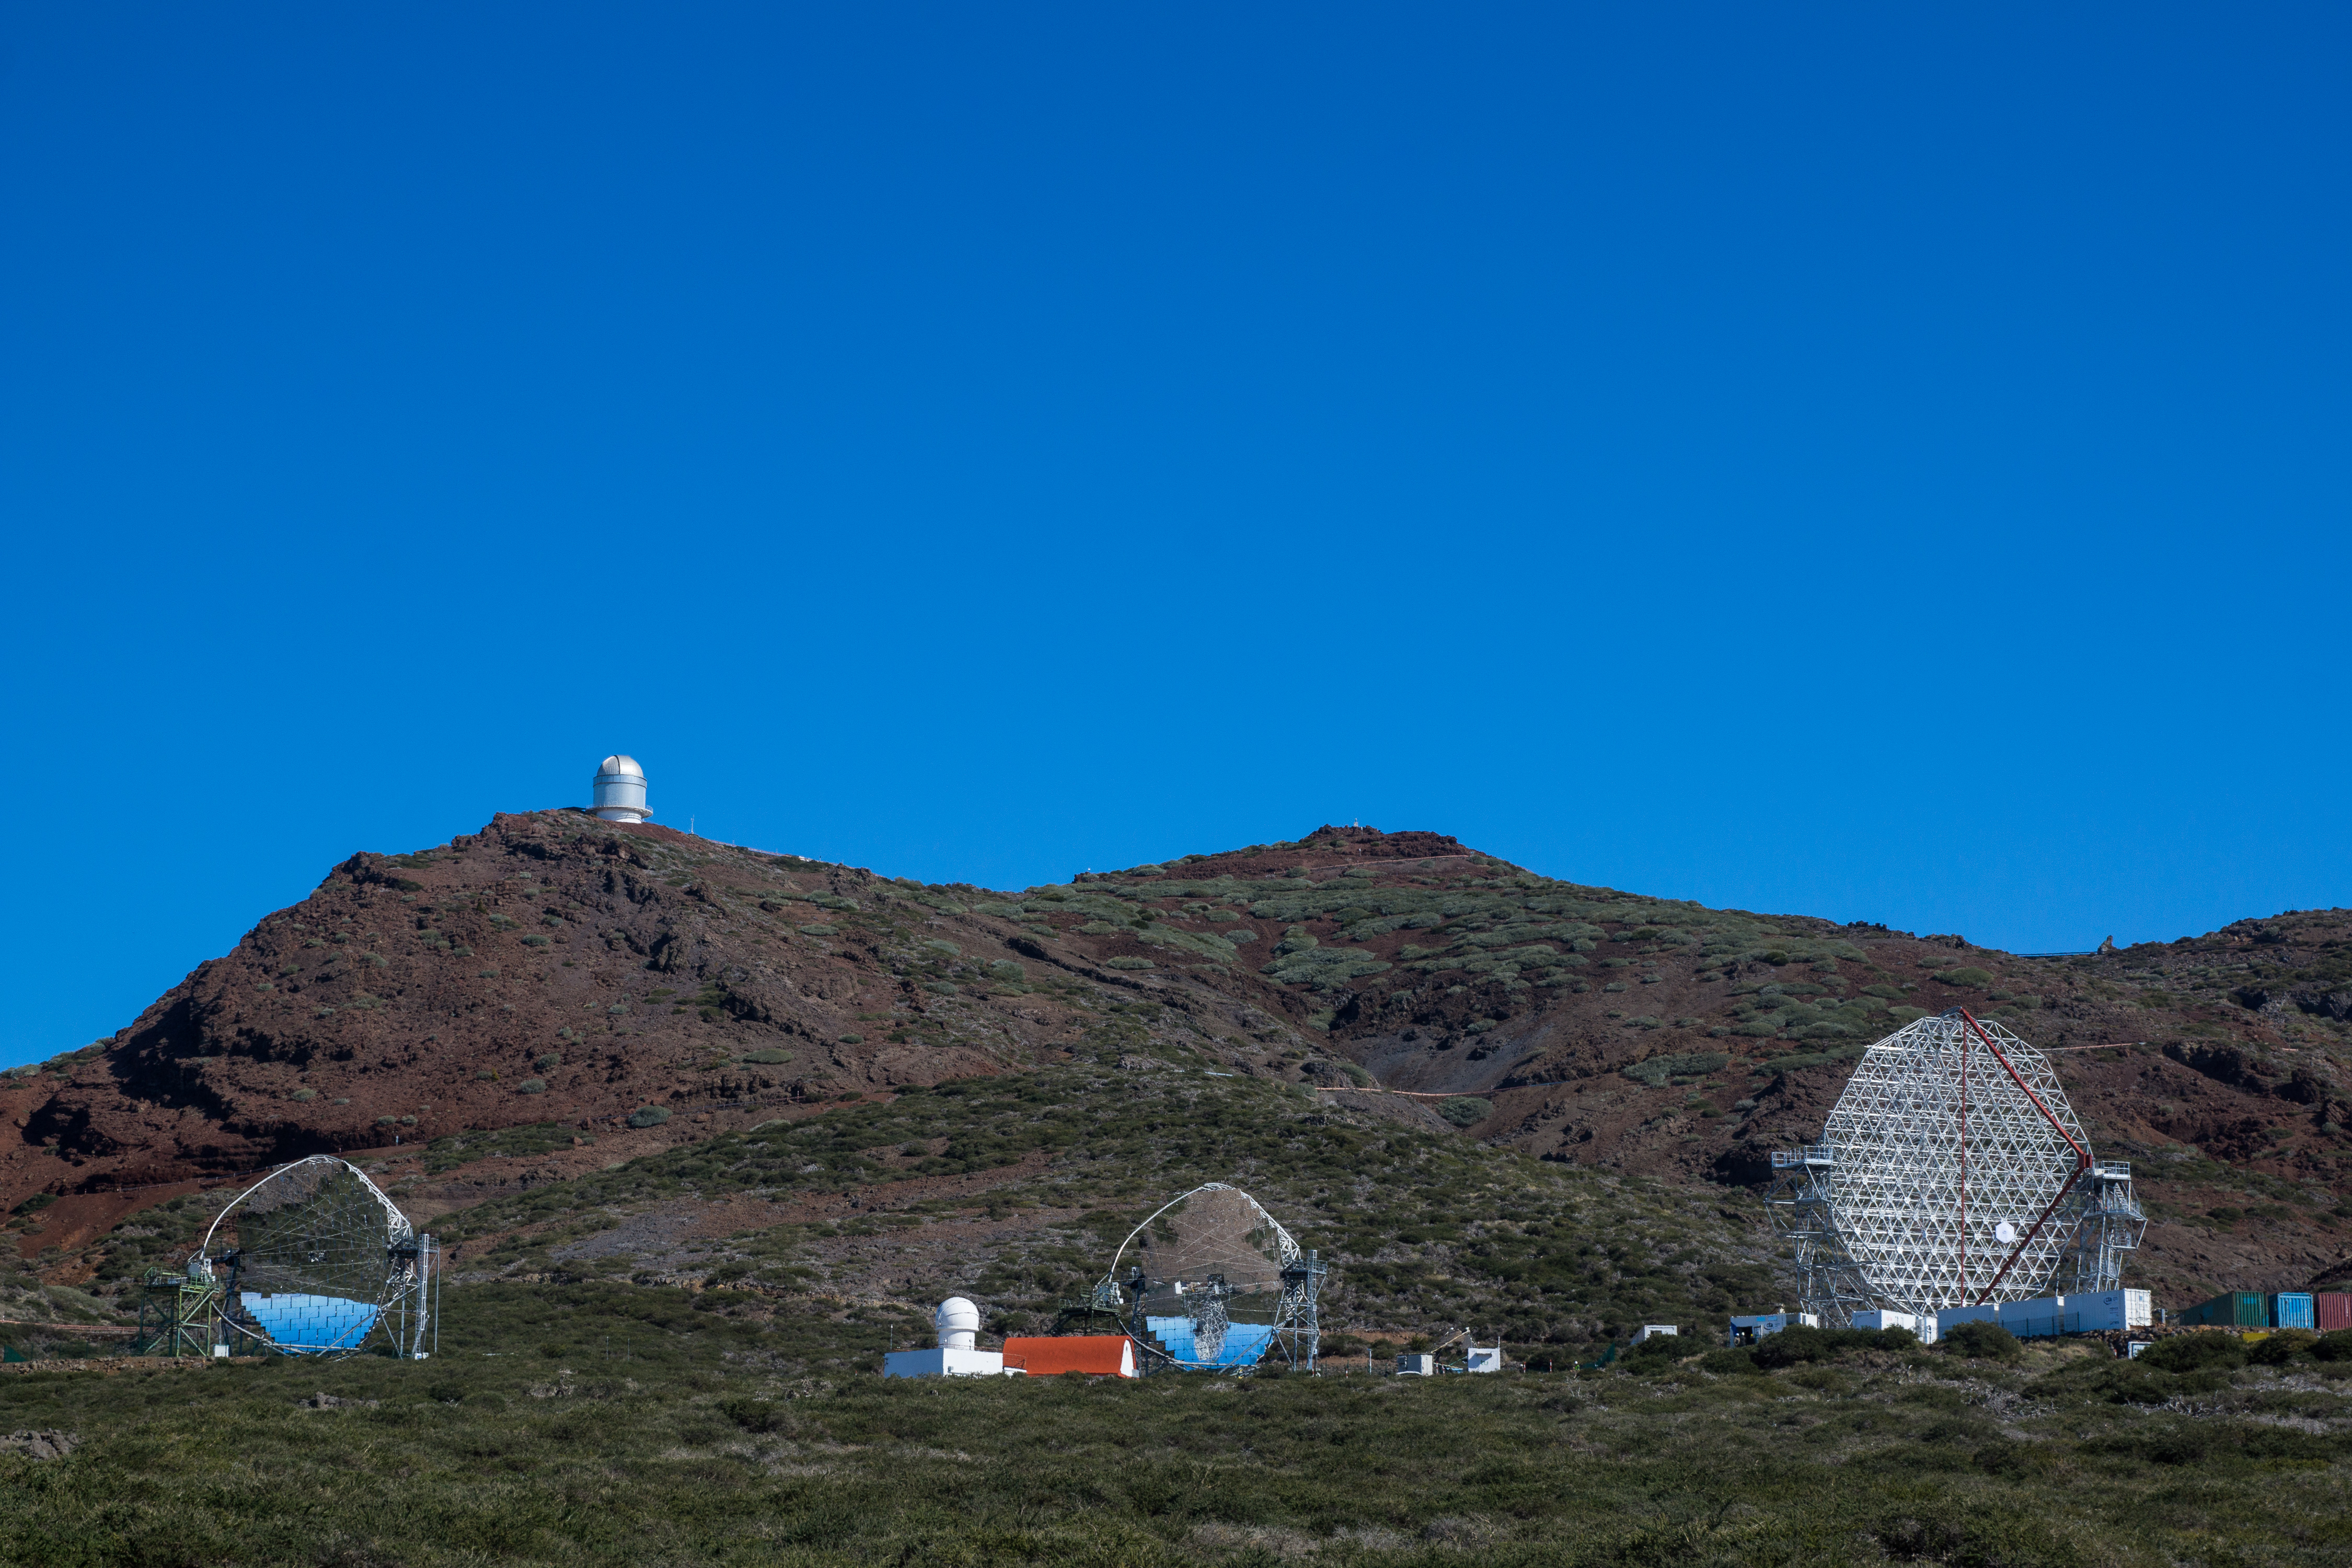
\includegraphics[width=\linewidth, trim={0 3cm 0 12cm}, clip]{images/magic_fact_lst.jpg}
  \caption{%
    The \gls{magic}, \gls{fact} and LST-1 telescopes (from left to right) at the \gls{orm} in April 2018,
    when the LST-1 was still under construction.
  }\label{fig:orm}
\end{figure}

To improve upon the sensitivity of the currently operating telescopes by at least 
an order of magnitude, both in the northern and the southern hemisphere, 
a large international consortium is currently planning and building the \gls{cta}.
In its final form, it will comprise 99 telescopes at the southern observatory in
Chile and 19 telescopes at the northern site at the \gls{orm}~\cite{science-cta}.
As of November 2019, prototypes for all of the three different telescope sizes
are developed and the first \SI{23}{\meter} Large Sized Telescope is in commissioning
at La~Palma and detected its first signal of the Crab Nebula~\cite{lst-crab}.
Construction of the full array will take several years and is currently planned
to be finished in 2025~\cite{cta-status}.

As one major open question is the variability of \glspl{agn}, see \autoref{sec:agn},
dense, unbiased\footnote{The currently observing large telescopes tend only to observe
\gls{agn} in active states when triggered through an external alert, thus having a
large selection bias on possible flux states.} monitoring of these objects is crucial to understand the underlying processes.
A possible solution for this would be to install Cherenkov telescopes around the globe
at multiple locations so that at least one telescope can observe a source at
any given time.
\gls{fact} was started as a prototype for a telescope in such a ring, but 
having larger telescopes with higher sensitivity for the short scale variability
would improve the possible scientific results dramatically~\cite{ctr}.

\subsection{Water Cherenkov Telescopes}

The third possibility of detecting high energy gamma-radiation is
measuring the energetic particles produced in air showers that reach the ground
using water Cherenkov tanks.
These large volume tanks contain photosensors that detect the Cherenkov light
produced by particles going through the water.
As these water tanks are closed, these observatories are not bound to observing
only in dark nights and are much less affected by weather conditions in comparison
to \glspl{iact}.
Also, they observe the whole sky above them at any given time, though 
sensitivity is limited beyond zenith distances of more than \ang{45}.
The only currently operating observatory using this detection mechanism is
the \gls{hawc} experiment in Mexico~\cite{hawc-monitoring}.
\gls{hawc} is fully operational using 300 water tanks with \SI{190}{\cubic\meter}
of water each since 2015, each tank is outfitted with four \glspl{pmt}~\cite{hawc-monitoring}.
\gls{hawc}'s sensitivity for point sources is lower than for most \glspl{iact} in the
common energy range, but it can monitor many sources at the same time.


\section{Sources of Gamma Radiation}\label{sec:sources}
\begin{figure}
  \centering
  \includegraphics{build/plots/4fgl_fact_sources.pdf}
  \caption{%
    The gamma-ray sky as observed by the Large Area Telescope aboard the 
    \textit{Fermi}-Satellite in equatorial coordinates and equal-area Mollweide projection.
    The color of the points indicates particle flux between \SI{1}{\GeV} and \SI{100}{\GeV}.
    A gray band shows the galactic plane.
    The seven sources most observed by \gls{fact} are marked. 
    All but the Crab Nebula, which is a \gls{snr}, are blazars.
    Data taken from the 4FGL~\cite{4fgl}.
  }\label{fig:4fgl}
\end{figure}
\noindent High energy gamma radiation can originate from two main source types.
Gamma rays from inside the Milky Way are mostly produced in super nova remnants,
mostly pulsars, \gls{pwn} and shell-type super novae.
Extragalactic sources are dominated by \glspl{agn}, the very bright central regions of galaxies containing super massive black holes with \num{e6} to \num{e10} solar masses $M_\odot$~\cite{app-angelis}.

\subsection{Active Galactic Nuclei}\label{sec:agn}
Outside of our own galaxy, the most numerous, lasting sources
of gamma radiation are \glspl{agn}, galaxies with super massive black holes at their centers.
These black holes accrete matter from the surrounding medium,
forming disks around the black hole.
These objects belong to the brightest in the universe, reaching powers
of \SI{e40}{\watt}~\cite{app-angelis}.
In some cases, narrow, relativistic jets of particles shoot out perpendicular to the accretion disk of matter falling into the black hole.
\begin{wrapfigure}[23]{O}{0.5\textwidth}
  \includegraphics[width=\linewidth]{images/m87.jpg}
  \caption{%
    Hubble image of the radio galaxy M87, an \gls{agn} with
    a larger viewing angle than blazars, so the relativistic jet is visible.~\cite{hubble-m87}.
    The central black hole of M87 was also the first to be directly imaged through
    \gls{vlbi}~\cite{m87-bh}.
  }\label{fig:m87}
\end{wrapfigure}

The jet producing \glspl{agn} are classified into categories based on the viewing angle
towards the jet.
A viewing direction nearly down the jet and the resulting Doppler-boosting classify an \gls{agn} as blazar
and these are the main sources of high energy, extra-galactic gamma rays.
Blazars are subdivided into two categories based on the existence
or absence of line emission in the optical spectrum.
\glspl{fsrq} show broad line emissions, likely from gas clouds closely orbiting the black hole, and generally have a higher energy output than
BL Lacertae objects, named after the prototypical source, 
that show no or very weak line emissions~\cite{fromblazars}.

While BL Lac objects have lower overall energy output, they reach
higher energies and are the predominant extra-galactic source type
at \si{\TeV} energies.
The 4FGL catalog contains 1109 BL Lac objects, 652 \glspl{fsrq} and 1310 blazars of
uncertain type~\cite{4fgl}.
Compared to that, TeVCat~\cite{tevcat},
an online catalog keeping track of gamma-ray observations at \si{\TeV} energies,
lists 52 BL Lac objects and only 6 \glspl{fsrq} to be detected in this energy range.

The gamma-ray flux of blazars is characterized over more than ten magnitudes
by a double hump structure. 
The first, low energy hump is universally assumed to be from synchroton radiation
of high energy electrons and peaks in the infrared to soft X-ray band.
The second, high energy hump is not fully understood and two main classes 
of models try to describe the high energy emission, either
purely leptonic models or models including hadronic components.

The simplest model describing gamma-ray flux from blazars is the single zone,
synchroton self-Compton model.
Assuming a single population of high energy electrons, low energy photons
are created by synchroton radiation and some of these photons gain energy
from the same population of electrons via inverse Compton scattering.
This scenario is purely leptonic and would not require high energy protons,
thus excluding these sources as possible origin of high energy cosmic rays.

However, some blazars show hints of a hadronic component, where additional
high energy photons are created by neutral pion decays~\cite{fromblazars}. 
As these hadronic reactions would also produce charged pions, which in turn
decay into neutrinos, observations of neutrinos from blazars would be the \enquote{smoking gun}
for blazars being sources of high energy cosmic rays.
A first strong hint for neutrinos from a blazar was published in 2018 by the
IceCube collaboration, where first a single, 
high energy neutrino from a direction consistent with the blazar TXS0506+056 
simultaneously with a flare in the electromagnetic spectrum of the source was observed~\cite{txs}.
In a second step, IceCube found an excess of lower energy neutrinos from the direction
of the source in historic data with a significance of \SI{3.5}{\sigma}~\cite{txs-historic}.

Blazars show large variability of their flux states,
both on long time scales slowly changing their mean power over months and years
and on very short time scales, doubling their flux in mere minutes, 
contesting the more simple models for blazar emission that cannot describe 
variability on such short timescales~\cite{fromblazars}.
In a very bright outburst in 2005, \gls{magic} observed a doubling of the flux of Mrk~501
in only two minutes~\cite{mrk501-variability}.

\subsection{Super Nova Remnants}
Most individual sources of gamma radiation in our own galaxy are the different types
of super nova remnants~\cite{tevcat, 4fgl}, what is left behind by the violent
death of a massive star.
Depending on the mass of the progenitor star and the age of the \gls{snr}, 
three related main classes exist: pulsars, \glspl{pwn} and shell-type \glspl{snr}.

% \begin{wrapfigure}[25]{O}{0.4\textwidth}
%   \includegraphics[width=\linewidth]{images/crab.jpg}
%   \caption{%
%     Multi-wavelength image of the Crab Nebula in pseudo-colors.
%     Observations of five different telescopes were combined:
%     VLA (radio, red), Spitzer Space Telescope (infrared, yellow), Hubble Space Telescope (visible, green),  XMM-Newton (ultraviolet, blue) and Chandra X-ray Observatory (purple)~\cite{crab-mwl}.
%     The central part dominated the purple X-ray observations shows the pulsar with its accretion disk and jet.
%   }\label{fig:crab}
% \end{wrapfigure}

\begin{figure}
  \begin{captionbeside}{
    Multi-wavelength image of the Crab Nebula in pseudo-colors.
    Observations of five different telescopes were combined:
    VLA (radio, red), Spitzer Space Telescope (infrared, yellow), Hubble Space Telescope (visible, green),  XMM-Newton (ultraviolet, blue) and Chandra X-ray Observatory (purple)~\cite{crab-mwl}.
    The central part, dominated by the purple X-ray observations, shows the pulsar with its accretion disk and jet.
  }%
    \small%
    \raisebox{\dimexpr\baselineskip-\totalheight\relax}{%
      \includegraphics[width=0.5\linewidth]{images/crab.jpg}
    }% 
  \end{captionbeside}\label{fig:crab}
\end{figure}

Stars are in an equilibrium between gravitational force trying to
collapse them and radiative pressure preventing this.
After a star burned through most of its hydrogen fuel,
the radiative pressure falls and the star starts to collapse until three helium nuclei can be fused 
into carbon and pressure is built up again keeping the star stable once more, now
burning through its helium supply.
This repeats several times—each time producing heavier elements—until iron is reached,
which is the last element where fusion produces energy.
If the remaining core is more massive than $\num{1.4} M_\odot$, the core collapses
into a neutron star, if the mass is larger than 3 to 5 times $M_\odot$, it will collapse 
into a black hole.
The collapse also results in the supernova explosion.~\cite{app-angelis}

Neutron stars are only \SIrange{10}{20}{\kilo\meter} in diameter and
rotate very quickly, because of the conservation of angular momentum
and show extreme magnetic fields up to \SI{e8}{\tesla}~\cite{app-angelis}.
If the rotation axis is not aligned with the magnetic field axis,
neutron stars are observed to emit pulsed beams of radiation,
These pulsars, found in most young \gls{snr},
are the most numerous galactic source type in the 4FGL catalog~\cite{4fgl}.
A pulsar can power gamma-ray emission in the surrounding gas cloud left over
from the supernova explosion, creating a \gls{pwn}.
The most prominent source of high energy gamma radiation, the Crab Nebula,
is a \gls{pwn} created by a supernova explosion in 1054, observed by Chinese
and Japanese astronomers, visible at daylight for 23 days~\cite{sn1054}.
A pseudo-color image of the Crab Nebula from multiple observatories is shown in \autoref{fig:crab}.

Particle acceleration happens very similar to the mechanisms proposed for \gls{agn}
and the Crab Nebula is particularly well described via a purely leptonic 
synchroton and inverse Compton model,
using two different electron spectra and four photon distributions: 
the synchroton radiation (the self Compton part), thermal emissions from dust, the
cosmic microwave background and line emission from the nebula~\cite{meyer-crab}.
The full spectral energy distribution from the radio regime to very high energy
gamma radiation as measured by several experiments is shown in \autoref{fig:crab-sed}.
The Crab Nebula also shows a rather constant flux at very high energies and
has thus become the \enquote{standard candle} of VHE gamma-ray astronomy~\cite{meyer-crab}.
The Crab Nebula is used as reference for sensitivities, also in this work, and
as a unit of flux: \SI{1}{CU} being the flux of the Crab Nebula either differential
at a certain energy or integrated over a specific energy range.
The \gls{magic} collaboration published a log-parabola parameterization of
the Crab Nebula flux  valid for the whole energy range observable by \gls{fact} in \cite{magic-crab}:
\begin{equation}
  \Phi(E) = \frac{\num{3.23e-11}}{\si{\TeV\cm\squared\second}}
  \left(\frac{E}{\SI{1}{\TeV}}\right)^{\num{-2.47} - \num{0.24} \log_{10}(\sfrac{E}{\SI{1}{\TeV}})}. \label{eq:magic-crab}
\end{equation}
This parameterization will be used as reference spectrum to calculate the weights
for simulated events in \autoref{chp:performance}.

\begin{landscape}%
  \sisetup{per-mode=reciprocal}%
  \input{build/plots/crab_sed.pgf}\\
  \captionof{figure}{%
    Spectral energy distribution of the Crab Nebula, data from 16 observatories,
    available in a single data file from \cite{gammapy-crab}. 
    The gray line shows the parameterization of the inverse Compton part of the spectrum
    from \cite{meyer-crab}.
  }\label{fig:crab-sed}%
  \sisetup{per-mode=symbol-or-fraction}%
\end{landscape}

\subsection{Gamma-Ray Bursts}

The third class of gamma-ray sources are the short, transient bursts of gamma radiation
which are also of extra-galactic origin.
Two classes of bursts exist, bursts with durations longer than two seconds are
currently thought to be caused by core-collapse super novae, they make up around \SI{70}{\percent}
of the detected bursts.
One source for the bursts shorter than two seconds was confirmed in 2017, 
when LIGO and VIRGO observed a gravitational wave event caused by the merger of two 
neutron stars and a \gls{grb} was detected \SI{1.7}{\second} after this signal by the \textit{Fermi} satellite. 
Later, the kilonova was observed and detected by 70 observatories all around the globe
and in Earth's orbit. 
This first event measured both electromagnetically and in gravitational waves
was named \enquote{Science Breakthrough of the Year 2017}~\cite{neutron-star-merger}
and was the first true multi-messenger observation.

\section{Key Science Questions}\label{sec:science}

Stefan Funk~\cite{funk-gamma} and the \gls{cta} Consortium~\cite{science-cta} identify the following
questions as most relevant to currently observing and planned gamma-ray observatories:

\paragraph{The Origin of Charged Cosmic Rays}
Since first discovered by Victor F. Hess in 1912~\cite{hess1912},
the origin of the charged cosmic rays remain largely unknown.
Several candidates have been proposed, but none identified with certainty.
If gamma-ray sources would be discovered to show spectra only explainable 
using hadronic models, this would offer a strong hint that those sources also produce
charged cosmic rays.
This can only be an indirect proof compared to neutrino observations,
which would directly point to hadronic reactions.

\paragraph{The Search for Dark Matter}
High energy gamma-ray astronomy is sensitive to annihilation lines
created by several proposed candidates for dark matter particles,
e.\,g.\ by two \glspl{wimp} converting into two gamma rays.
Also theories for axion-like particles will be tested via the proposed changes to the
mechanics of the \gls{ebl} absorption.

\paragraph{Understanding Acceleration Mechanisms}
The precise mechanisms at work in the extreme environments of
\gls{agn} and pulsars are still a largely open question, 
especially the very short time scale variability is not described by current models.

\paragraph{Cosmology and Fundamental Physics}
\glspl{iact} are able to test a number of predictions made by 
several theories of quantum gravity, e.\,g.\ Lorentz invariance violations.
This is also connected to the question of dark matter.

\section{Cosmic Rays}\label{sec:cosmic-rays}
Charged primary particles are the main background class for any
gamma-ray telescope, also for \glspl{iact}.
As they are deflected by magnetic fields in the interstellar and
intergalactic medium, their origin is not reconstructible at rigidities 
relevant to \glspl{iact} and they thus form an isotropic, diffuse background.
\begin{figure}
  \centering
  \includegraphics{build/plots/proton_helium_spectrum.pdf}
  \caption{%
    Particle flux of protons (solid colors) and
    helium nuclei (transparent) as measured by several experiments.
    Data from \cite{cr-database}.
    The two gray lines are the respective fit results shown in \eqref{eq:proton-flux} and
    \eqref{eq:helium-flux}.
  }\label{fig:cr-flux}
\end{figure}

\autoref{fig:cr-flux} shows the flux of primary protons and helium nuclei between
\SI{1}{\GeV} and \SI{1}{\peta\eV}. 
These two elements make up over \SI{90}{\percent} of the charged cosmic rays
around \SI{1}{\GeV}~\cite{pdg}. 
At the energies relevant for \gls{fact}, above \textasciitilde\SI{100}{\GeV},
helium nuclei are almost as abundant as protons.
The flux of all charged primaries can be approximated above $\approx \SI{100}{\GeV}$
using
\begin{equation}
  I_N(E_N) \approx
  \frac{\num{1.8e4}}{\si{\GeV\meter\squared\second\steradian}}
  \left(\frac{E_N}{\SI{1}{\GeV}}\right)^{\num{-2.7}}
  \quad \text{\cite[(29.2)]{pdg}} \label{eq:all-particle}
\end{equation}
where $E_N$ is the energy \emph{per nucleon}.

The individual spectra for proton and helium nuclei are described using power laws
obtained by linear regression of $\log_{10}(I)$ vs. $\log_{10}(E)$ using
the data shown in \autoref{fig:cr-flux}.
For the proton flux, this yields
\begin{equation}
  I_\text{p}(E) = \frac{\input{build/proton_norm.tex}}{\si{\GeV\meter\squared\second\steradian}}
  \left(\frac{E}{\SI{1}{\GeV}}\right)^{\input{build/proton_index.tex}}
  \label{eq:proton-flux}
\end{equation}
and for the helium flux per nucleus, \emph{not nucleon},
\begin{equation}
  I_\text{He}(E) = \frac{\input{build/helium_norm.tex}}{\si{\GeV\meter\squared\second\steradian}}
  \left(\frac{E}{\SI{1}{\GeV}}\right)^{\input{build/helium_index.tex}}
  \label{eq:helium-flux}
\end{equation}
is obtained.
The covariance matrices for the fits are given in Appendix~\ref{apx:fit-results}.


For an observation of the Crab Nebula, the ratio
of gamma rays from the source to cosmic ray background events will approximately be
\begin{align}
  \frac{N_\gamma}{N_\text{CR}} &=
  \frac%
  {\int_{\Emin}^{\Emax} \int_A \int_{t_0}^{t_1} \Phi(E) \d{t} \d{A} \d{E}}%
  {\int_{\Emin}^{\Emax} \int_A \int_\Omega \int_{t_0}^{t_1} I_N(E) \d{t} \d{\Omega} \d{A} \d{E}}\\
  \intertext{%
    where $\Phi$ is the flux of the Crab Nebula, which for most \glspl{iact} can
    be assumed to be a point source and thus no integration over the solid angle is necessary.
    We can now calculate this ratio for an \gls{iact} with a field of view with a diameter
    of \SI{4.5}{\degree}, resulting in $\Omega = 2\PI (1 - \cos{\SI{2.25}{\degree}})\, \si{sr} \approx \SI{0.005}{\steradian}$. 
    The area of the detector and the observation time is the same for both terms and
    cancels out.
  }%
  \frac{N_\gamma}{N_\text{CR}} &= \frac%
  {\int_{\Emin}^{\Emax} \Phi(E) \d{E}}%
  {\SI{0.005}{\steradian} \int_{\Emin}^{\Emax} I_N(E) \d{E}}
  \intertext{using the log-parabola parameterization of the Crab Nebula flux published by
  the \gls{magic} collaboration in \cite{magic-crab} and an energy range of \SI{100}{GeV}
  to \SI{200}{\TeV} results in}
  \frac{N_\gamma}{N_\text{CR}} &\approx \frac{1}{4300}
\end{align}

So for each gamma-ray induced shower, 4300 showers induced by charged cosmic rays
are reaching the telescope.
We will see in \autoref{sec:sensitivity} that \gls{fact} can detect sources with down to \SI{10}{\percent} 
of the flux of the Crab Nebula in \SI{50}{\hour} of observation time, 
\gls{magic} is an order of magnitude more sensitive reaching around one percent
in \SI{50}{\hour} \cite{magic-performance}.
This directly translates into the ratio of signal to background events and
will necessitate an analysis that can classify recorded events as either 
gamma-ray or cosmic-ray induced to suppress this background as much as possible.
Methods to achieve this will be introduced in \autoref{chp:reconstruction}.

\chapter{The First G-APD Cherenkov Telescope}\label{chp:fact}
\begin{figure}
  \centering
  \includegraphics[width=\textwidth]{images/fact.jpg}
  \caption{%
    \gls{fact} in front of the \gls{magic}-II telescope at the Observatorio del Roque de los Muchachos.
    The white cylinder on the left is the camera, complete with all readout electronics.
    }%
  \label{fig:a}
\end{figure}


\noindent In this chapter, I will introduce the necessary aspects
of the \gls{fact} telescope, which are needed to understand the simulation
and analysis presented in the next chapters.

After a general introduction,
I will focus mainly on the data acquisition and electronics,
as these are the parts of the telescope that are most crucial for my work
on improving preprocessing of raw data and simulations.

\begin{wrapfigure}[25]{O}{0.55\textwidth}
  \centering
  \includegraphics{build/plots/fact_ontime_half.pdf}
  \caption{%
    Observation time for the seven sources most observed by \gls{fact}. 
    Together they amount to over \SI{95}{\percent} of the total time the telescope
    has observed.
  }\label{fig:obstime}
\end{wrapfigure}

One of the main goals of \gls{fact} was to demonstrate the possibility
of using \glspl{sipm} for Cherenkov astronomy~\cite{fact-design-operation}.
It has been the first telescope to employ this new technology of photodetectors
in the field when it started operating in 2011.
Now, eight years later, all prototypes for the \gls{sst} for \gls{cta} are based 
on \gls{sipm} cameras and the final design was agreed upon in 2019~
\cite{sst-harmonization}. 
It can be safely concluded that \gls{fact} reached this goal.

Compared to the traditionally used \glspl{pmt},
these semiconductor photosensors are much more robust to high light levels.
Due to this, \gls{fact} can observe under light conditions,
e.\,g.\ in moonlit nights, where other \glspl{iact} can not~\cite{fact_full_moon}.
This makes \gls{fact} uniquely suited for its main physics goal,
to monitor the brightest sources of gamma rays as densely as possible,
which is also evident in \autoref{fig:obstime},
showing that \gls{fact} spends most of its observation time on just seven sources.
Shortly after starting observations in October 2011,
the \gls{fact} collaboration started publishing
results of a \enquote{quick look analysis}~\cite{qla} as soon as they were available.
This analysis provides gamma-ray event rates normally around 20 minutes after the last event of a run was taken.
Based on this analysis, the \gls{fact} collaboration has issued
several alerts to the other \glspl{iact} to inform them of unusually bright
flux of the monitored sources~\cite{fact_alerts}.

\gls{fact} is build upon the refurbished mount of the former \gls{hegra} CT-3 telescope,
equipped with new drive motors, mirrors and the \gls{sipm} camera.
Compared to the other currently operating telescopes, like \gls{veritas} or \gls{magic},
\gls{fact} is rather small, limiting its sensitivity to the brightest sources.
It is also the only currently operating monoscopic Cherenkov observatory.
\gls{fact}'s reflector is a segmented mirror with 30 individual hexagonal facets,
creating a total reflective surface of \SI{9.5}{\square\meter} with approximately four
meters in diameter.
Each mirror as a focal length of \SI{4.9}{\meter}, which is also the effective focal 
length of the segmented reflector.
The facets were oriented in the Davies--Cotton-Design\cite{davies-cotton} before this
was changed to a hybrid between Davies--Cotton and a parabolic orientation
in May 2014, as a compromise between spatial and temporal resolution of the reflector system~\cite{mirror-alignment}.
At this point, the mirrors were also realigned, resulting in an overall better resolution
than before.

\section{Photosensors and Readout Electronics}\label{sec:camera}

\gls{fact}'s camera comprises 1440 pixels,
each consisting of a \SI{3}{\milli\meter} by \SI{3}{\milli\meter} \gls{sipm}
that is subdivided into 3600 individual \gls{gapd} cells.
\glspl{gapd} are photodiodes operated with a reverse bias above the breakdown voltage,
the limit above which a single electron/hole pair created by an absorbed photon can induce an avalanche.
The cell is connected in series to a resistor and the current created
by the avalanche results in dropping the bias below the breakdown breakdown, 
stopping the avalanche.
After an avalanche, the cell needs a short time to reset to the full bias voltage again.
During the dead time, while the cell is below the breakdown voltage,
no new signal can be created.
While it is above the breakdown but below the nominal operation voltage—called recovery time—,
the signal is lower than normally~\cite{fact-design-operation}.
The single cells are connected in parallel to form a single, accumulated output signal
per pixel.
\glspl{sipm} do not need a high voltage supply in the \si{\kilo\volt} regime like \glspl{pmt} do.
\gls{fact}'s photosensors have a breakdown voltage around \SI{70}{\volt} and
are operated at an overvoltage of \SI{1}{\volt}, 
while some more recent models even only require \SI{30}{\volt}~\cite{sensl}.

However, \glspl{sipm} do not come without issues.
One disadvantage is the temperature dependent gain of \glspl{sipm} and two
main approaches exist to deal with this: active cooling of the sensors to a
fixed temperature or a system adjusting the bias voltage of the \glspl{sipm} 
so the gain stays stable.
\gls{fact} has implemented the second path, only relying on removing excess heat
from the camera, not keeping a fixed temperature for observations.
The bias voltage is generated in the container next to the telescope and supplied
to groups of 4 or 5 pixels, called bias patches shown in \autoref{fig:pixels}.~\cite{fact-design-operation}

Compared to \glspl{pmt} they have a higher dark count rate,
signals induced not by photons but by thermal electrons in the sensor itself.
Cross talk, the effect that a break through in one cell can trigger another in a neighboring cell,
results in a signal corresponding to two photons or more.
There is also a chance  that a discharge triggers a later discharge of the same cell,
which is called an after pulse.~\cite{cross-talk}

To increase the light gathering surface area, a Winston cone with a hexagonal
entry window with an incircle diameter of \SI{9.5}{\milli\meter} is placed in front of each pixel.
The resulting camera is roughly \SI{40}{\centi\meter} in diameter which, together with
the \SI{4.9}{\meter} focal length of the reflector, gives a field of view of \SI{4.5}{\degree}.
Each individual pixel covers \SI{0.11}{\degree} in diameter on the sky.

\begin{figure}
  \begin{captionbeside}{
    Schematic view of the camera. From left to right: the 1440 pixels in the 
    sensor compartment, the insulation between sensor compartment and
    readout electronics, the 4 crates with the preamplifier boards and the 
    \gls{fadc} boards. The \gls{ftm} can be seen at the top next to the insulation.\\\relax
    [Graphic by Sebastian~A.~Mueller]
  }
    \raisebox{\dimexpr\baselineskip-\totalheight\relax}{%
      \includegraphics[width=0.6\linewidth]{images/image_sensor.pdf}
    }% 
  \end{captionbeside}\label{fig:camera}
\end{figure}

The analog signal of the pixels is wired to the preamplifier boards, that handle
36 pixels each and are organized in four crates of ten boards of the preamplifier
and \gls{fadc} boards each.
The trigger unit on the preamplifier board clips and sums the signal of 9 pixels each,
these groups are referred to as trigger patches. 
The preamplifier board applies an $N$-out-of-four logic to these trigger input signals,
which is the input for the \gls{ftm} board, which applies a $N$-out-of-40 logic to
decide if an event should be stored to disk.
For normal physics observations, both $N$ are 1, thus if any of the 160 trigger patches
is above the trigger threshold, an event is stored to disk.
In addition to events triggered by this system, additional events are recorded
during normal data runs.
The camera is read out once per second regardless of a trigger signal, these
are so called interleaved pedestal events which can be used to estimate the noise
level.
Since November 2013, the camera is also triggered at every full second by a GPS
receiver to provide more precise timing information.
Until 2017, an LED light pulser in the reflector dish fired every few seconds,
this was done for calibration of the pixel response.
However, this LED light pulser went rogue in 2015 and also fired without being activated
creating large events triggered by the physics trigger until it was finally removed in April 2016.

The \gls{fadc} boards also receive their signal from the preamplifier boards.
The heart of the \glspl{fadc} are the \gls{drs4} chips~\cite{drs4}. 
These chips sample the analog signal using 1024 capacitors for each channel using
a sampling frequency of \SI{2}{\giga Sample \per \second}.
In case the \gls{ftm} issues a trigger decision, the voltage stored in the capacitors
is readout and digitized by a 12-bit \gls{adc}.
For regular observations, only 300 of the samples are readout, starting 50 samples
before the trigger signal was received \cite{fact-design-operation}.
While the \gls{drs4} chips allow fast digitization of the \gls{sipm} signal,
it also introduces the need for several calibration steps
and adds artifacts to the data~\cite{magic-drs4}.
The most common artifacts are sudden increases of the digitized signal in a single
or two adjacent cells called spikes.
These interfere with the searching for the Cherenkov pulse signal if not corrected.
Different amounts of remaining charge in the cells are responsible for sudden shifts of the baseline
for longer time periods when reading out cells that have had different times since their previous readout.
In \gls{fact}'s terminology, these are called jumps.

The digitized samples are transferred via four ethernet connections to the data acquisition computer which writes the data to disk. 
Under good environmental conditions \gls{fact} triggers between 60 and 80 events per seconds
\cite{fact-sipm-performance,fact-design-operation}.
The organization of the \gls{fact} camera pixels into the different groups is shown in
\autoref{fig:pixels}.

\begin{figure}
  \centering
  \includegraphics{build/plots/fact_pixels.pdf}
  \caption{%
    Organization of the \gls{fact} camera.
    The four main colors highlight the crates, the variation in those colors the 
    boards.
    The left image shows the individual pixels.
    In the central image, pixels using the same bias voltage supply are grouped.
    The right image shows all pixels on the same \gls{drs4} chip, which also corresponds
    to the trigger patches.
  }\label{fig:pixels}
\end{figure}

\section{Observation Strategy}\label{sec:wobble}

As not all recorded background events can be discarded reliably while still
keeping most of the gamma rays, a method to estimate this residual background is needed.
A simple method would be to observe the gamma-ray source first and then 
observe a similar region in the sky without a gamma-ray source for the background estimation.
This has several important drawbacks,
first the available time for source observations is cut in half.
Second, the observation conditions might change and thus bias the estimation of the background.

A way around this is not to position the source of interest in the center of the 
camera but using a small offset.
In this case, several regions in the camera geometrically
equivalent to the position of the gamma-ray source can be used for the background estimation.
This maximizes observation time for gamma-ray sources, guarantees identical observation
conditions for the background estimation and also decreases the
statistical uncertainty for the background, as several positions can be used~\cite{wobble}.
The situation is sketched in \autoref{fig:wobble}.
Nearly all \gls{fact} observations are carried out in this manner.
Due do the characteristic switching between positions relative to the source,
making small jumps around its position, this strategy is called \enquote{wobble mode}.

\begin{figure}
  \centering
  \begin{tikzpicture}
  \newlength\mydeg
  \setlength{\mydeg}{2cm}

  \pgfdeclarelayer{bg}
  \pgfsetlayers{bg,main}

  
  \node[star, star points=5, fill=yellow!80!red, minimum height=0.3cm] (source)  at (0, 0) {};

  \node[draw=darkBlue, cross out, line width=2pt, minimum height=0.3cm] (p1) at (-0.6\mydeg, 0) {};
  \node[draw=darkRed, cross out, line width=2pt, minimum height=0.3cm] (p2) at (0.6\mydeg, 0) {};

  \begin{pgfonlayer}{bg}
    \draw[thick, black!20, dashed] (p2) circle (0.6\mydeg);
    \draw[thick, black!20, dashed] (p1) circle (0.6\mydeg);
  \end{pgfonlayer}

  \draw[thick, darkBlue] (p1) circle (2.25\mydeg);
  \draw[thick, darkRed] (p2) circle (2.25\mydeg);

  \foreach \ang in {60,120,180,240,300} {
    \path (p1) -- ++ (\ang:0.6\mydeg) node[circle, minimum height=0.3cm, fill=blue!50!black] {};
  }
  \foreach \ang in {0,60,120,240,300} {
    \path (p2) -- ++ (\ang:0.6\mydeg) node[circle, minimum height=0.3cm, fill=red!50!black] {};
  }

  \draw[{Bar[]Triangle[]}-{Triangle[]Bar[]}] ([yshift=-0.3cm]p1.center) -- ([yshift=-0.3cm]source.center) node [midway, above] {\SI{0.6}{\degree}};
\end{tikzpicture}

  \caption{%
    When observing a source in wobble mode, the source (yellow star) is not in the center (crosses) of the field of view but offset by a certain amount.
    \gls{fact} uses \SI{0.6}{\degree}. 
    Shown here are two wobble positions at wobble angles of \SI{0}{\degree} (red) and \SI{180}{\degree} (blue) as measured from the right ascension axis.
    \gls{fact} normally observes using two wobble positions at \SI{180}{\degree} offsets,
    changing position every twenty minutes.
    The bold circles show the five off positions per pointing position that are
    used to estimate the background.
    Because there is a bright star in the field of view for Crab Nebula observations,
    the wobble angles are shifted by \SI{50}{\degree}, so the star is not close to
    any of the off positions.
  }\label{fig:wobble}
\end{figure}

\chapter{Monte Carlo Simulation of FACT Events}\label{chp:simulation}

To evaluate the performance of an instrument design before it is build
or to generate labeled data for the training of statistical models,
the possibility of simulating the data of instruments is of crucial importance.
As there are no artificial sources of gamma rays and cosmic rays at the energies
measured by \glspl{iact}, extensive simulations are
necessary to be able to reconstruct the events observed with these telescopes.

Simulation of events for \glspl{iact} is usually done in two steps:
First, the \gls{eas} is simulated which produces the Cherenkov light
on the ground level at the telescope as output.
Second, from the simulated Cherenkov photons, the detector response
of the instrument is calculated.

Due to the stochastic nature of the involved processes, the Monte Carlo
method is the perfect fit to generate artificial \gls{iact} events with known
initial conditions.
Very few initial parameters result in an incalculable large number of possible outcomes.
Simulating a single air shower requires drawing several million pseudo random numbers.

For small instruments like \gls{fact}, the simulation of the \gls{eas} is
usually much more computationally intensive than the simulation of the detector response.

\section{Simulation of Air Showers Using CORSIKA}\label{sec:corsika}

The development of \gls{corsika}~\cite{corsika} initially began in the late 1980s by merging
three precursor code bases into a single software to simulate \gls{eas} for
the KASCADE~\cite{kascade} cosmic ray experiment.
It was later extended to also be able to calculate Cherenkov light production,
currently with the \texttt{iact/atmo} extension \cite{iactatmo}.

\gls{corsika} simulates all particle interactions from the moment
a particle enters Earth's atmosphere.
This requires knowledge of the cross-sections for all possible processes,
especially for very high energy interactions in forward direction and for
air molecules.
These regimes are generally not accessible by collider experiments and
are thus extrapolated from the available data at lower energies, larger
scattering angles and other nuclei~\cite{epos-lhc}.
Improvements to the cross-section calculations after new experimental data
is published is one of the main improvements between \gls{corsika} versions.

To produce simulations with \gls{corsika}, a large number of configuration options
have to be considered, both at compile and run time.
These need to be adapted for the specific experiments and several libraries
can be chosen for the calculation of the particle interactions.

\gls{corsika} is written in \texttt{FORTRAN 77},
while the \texttt{iact/atmo} extension is written in \texttt{C}.
Unfortunately, \gls{corsika} is not Free and Open Source Software.
However, access is usually granted for anyone interested in using the software.
There is an ongoing effort to create the next major version of \gls{corsika} 
using more modern technologies in a complete redesign,
openly developed by the community and published under an open source license.
However, this is not yet finished as of early 2020~\cite{corsika8}.

In this work, new simulations were produced using \gls{corsika}, version \texttt{7.69} released in December 2018 of \gls{corsika}.
These are compared to simulations that were previously created 
by the \gls{fact}-Collaboration
using a customized version of \gls{corsika} called \gls{mmcs}, which
was based on version \texttt{6.5} \cite{mmcs}, released in 2006.

\subsection{Interaction Models}\label{sec:models}

The particle interaction cross sections are not calculated by \gls{corsika} itself
but by externally contributed libraries.
When simulating Cherenkov light, 
the electromagnetic interactions are simulated using \gls{egs4}~\cite{egs4}.

For the hadronic interactions, several libraries are available for use
with \gls{corsika}.
As these libraries have their own energy domains, \gls{corsika} splits 
calculations into two energy regimes each handled by a different library with
a hard transition at \SI{80}{\GeV}~\cite{corsika_manual_769}.
Choosing the libraries for the different cross section calculations is a compile time option.

There are three possible choices for the hadronic interactions below an energy of
\SI{80}{\GeV} in \gls{corsika} 
for both versions \texttt{7.69} and \texttt{6.5}: \gls{gheisha}, \gls{fluka} and \gls{urqmd}~\cite{corsika_manual_769}.
According to a comparison of the three models in \cite{model_comp_auger}, \gls{gheisha} fails to reproduce measured data when used with \gls{corsika} to simulate air showers.
It was thus not considered for the simulation of \gls{fact} events.
\gls{fluka}~\cite{fluka} is only provided as compiled binary to registered users with a very restrictive
license~\cite{fluka-license}.
These binaries even have a \enquote{shelf life} date compiled into them,
after which the software will stop to work.
As this is all but prohibiting the reproducibility of the simulations, 
\gls{fluka} should not be used for a new set of simulations.
However, for a long time it was considered to be the best model~\cite{model_comp_auger} and it was used
to produce the simulations with \gls{mmcs} \texttt{6.5}.
\gls{urqmd}~\cite{urqmd}, the third option, will be explored as an alternative to 
\gls{fluka}.

The possible choices for the hadronic interaction models above \SI{80}{\GeV} are more numerous,
with some of the options being combinations of the other models.
The \gls{mmcs} \texttt{6.5} production used \gls{qgsjet}.
With the advent of \gls{LHC} measurements, many libraries were updated to reproduce the 
now available data at higher energies and for lead collisions~\cite{epos-lhc}. 
Together with the \texttt{iact/atmo} extension discussed in the next section,
these are the major changes from using \gls{mmcs} \texttt{6.5} to \gls{corsika} \texttt{7.69}.
The most advanced model is currently \texttt{EPOS-LHC}~\cite{epos-lhc}, which combines the older
\texttt{VENUS} and \gls{qgsjet} models with better extrapolation and \gls{LHC} data.


\subsection{Cherenkov Light Production}\label{sec:corsika-cherenkov}

Any charged particle traveling faster than the local speed of light induces
emission of Cherenkov light.
\gls{corsika} divides the tracks of particles into steps between interactions,
decays or the deflection in Earth's magnetic field.
These track parts along with start and end energy of the particle are
handed over to the subroutines calculating the Cherenkov emission.

A first version of the Cherenkov production code, used by the \gls{mmcs} \texttt{6.5}
production, was developed for non-imaging detectors of the \gls{hegra} array and proofed
to be not ideal for \glspl{iact}.
The later developed \texttt{iact/atmo} extension improves several aspects:
photons are collected in spheres encompassing the telescopes instead of
rectangles on the ground,
better description of the atmosphere by using fine-grained, tabulated values
for density and refractive index and taking atmospheric refraction of the Cherenkov
photons into account~\cite{iactatmo}.
Due to these improvements, the \texttt{iact/atmo} extension will be used for the
new simulations using \gls{corsika} \texttt{7.69}.
The \texttt{iact/atmo} extension writes its output in the \texttt{eventio} format~\cite{eventio},
a generic container format for binary payloads,
which are defined by the applications writing and reading the data.
Two different formats exist for the Cherenkov payload,
a smaller representation called \enquote{compact} 
with limited precision using 16-bit integers to store scaled quantities and a larger
storing 32-bit floating point values.

Both the \texttt{iact/atmo} extension and \gls{mmcs} offer the possibility
to \emph{reuse} a shower.
Meaning that the same telescope is randomly placed at different 
positions in the Cherenkov light pool of a shower,
effectively creating multiple events from the same air shower.
This results in a very direct speed up of simulations and since
most of the simulated showers will not trigger the telescope or survive
the event selection in the analysis, it is quite rare that the same shower 
is used multiple times in the end, which could introduce a statistical
bias as events would not be independent anymore.
Because computation time and small event numbers are mainly a problem of 
hadronic simulations, a reuse of 20 is only used for these showers and not for photon primaries.
Another option of improving simulation performance is treating several photons
as a single ray with a weight corresponding to the number of photons.
This is called bunching and is a compromise between accuracy of the spatial 
distribution and computing time.

Because \gls{fact}'s photo detectors are sensitive to larger wavelengths then
classical \glspl{pmt}, Cherenkov photons are simulated in wavelengths from \SIrange{290}{900}{\nano\meter}.  

\subsection{Particle Properties and Other Configuration Options}
All runtime options for an individual corsika run, meaning a single execution of
the program simulating a fixed number of showers, are configured in a 
plain text file called the input card.
This includes properties of the primary particles, 
description of the telescopes, seeds for the random generator to ensure
reproducibility, the local magnetic field, the atmosphere and many more.

The initial parameters of any particle in the simulation are
\begin{itemize}[nosep]
  \item Particle type
  \item Energy
  \item Direction
  \item Position, expressed as the impact point on the ground for primaries.
\end{itemize}
At the beginning of each new simulation event, these properties are either
fixed or drawn randomly from the corresponding distributions.
In the simulations done for \gls{fact}, the particle type
is always kept fixed, either gamma rays, protons or helium nuclei are simulated.
The energies of the simulated events are drawn from a power law distribution with
spectral index $\gamma$ between a minimum ($\Emin$) and a maximum energy ($\Emax$).
The distance to the telescope $R$, also known as the impact parameter,
is drawn so that the events are inside a circle of radius $R_{\max}$ and uniform in area.
The direction is sampled uniformly in the azimuth angle $φ$ between $φ_{\min}$ and
$φ_{\max}$
and the zenith angle $ϑ$ is sampled to be uniform in solid angle between $ϑ_{\min}$
and $ϑ_{\max}$.
The corresponding probability density functions are given in Appendix~\ref{apx:corsika-pdfs}.

\section{Simulation of Detector Response using CERES}\label{sec:ceres}

The detector simulation of \gls{fact} is done using \ceres{}~\cite{ceres}, an executable
using \gls{fact}'s version of the \gls{mars}\footnote{While sharing a common history, developement of \gls{fact}'s and \gls{magic}'s version of the software split before \gls{fact} started operation in 2009. \gls{magic}'s version is not public.} framework to simulate the detector response
given Cherenkov photons on the ground as input.
\ceres{} supports both the classical \gls{corsika} binary output format and the \texttt{eventio}
output format produced by the \texttt{iact/atmo} extension as discussed in the \hyperref[sec:corsika]{previous section}. 
Reading of \texttt{eventio} however is rudimentary and does not support all features
of \gls{corsika}, e.\,g.\ only a bunchsize of 1 and the compact format of the \gls{corsika}
output are supported.
As with \gls{corsika}, \ceres{} has a multitude of configuration options,
describing the telescope, the pointing position relative to the shower axis and the environmental conditions.

The first step in the simulation in \ceres{} is the application of several absorption
processes, reducing the amount of photons the simulation needs to process.
As each photon that finally might be detected in one of the telescope's pixels 
goes through the same processes that might absorb the photon, all of these
processes can be combined into an overall detection efficiency, greatly reducing 
computational cost through applying this absorption as early as possible.
These absorptions include atmospheric scattering, reflectivity of the mirrors,
transmittance of the entrance window of the camera and the Winston cones and
the photon detection efficiency of the \glspl{sipm}.
All these efficiencies are tabulated vs.\ wavelength in files as input to the simulation.
For the simulations produced for \cite{phd-temme}, an additional absorption without
direct physical cause further reducing the number of photons was introduced.
This is used to model all neglected sources of photon loss, like shadowing effects
of the mast structure holding the camera.

After discarding photons according to the overall absorption,
simplified ray tracing is done to simulate the optical system,
calculating which pixel if any is hit by the photon.
The segmented mirror is defined in a configuration file,
providing shape, size, focal length, position and orientation of each facet.

The signal of the \glspl{sipm} is calculated by superimposing the pulse shape
of a single photon for each individual photon, also adding additional photons
for the \gls{nsb}, dark counts and cross talk.
The pulse shape can either be defined using tabulated values in a text file
or an analytical function.
An additionial electronic noise, only simulated as simple white noise is added to the resulting signal.

Several options to further add artifacts to the simulated timeseries 
were implemented for the simulations produced for \cite{phd-temme}.
It was observed that the temporal features are not well-described, 
especially the variance of photon arrival times was much smaller for simulated
events than observed on measured data.
Three different approaches were introduced to tackle this problem:
a fixed time offset for each pixel, so that the signals would go out of sync,
a random offset between pixels for each event and smearing the arrival times
of each individual photon by a normally distributed random number.

The signal is then used to simulate the trigger decision and if any trigger
is raised, the event is stored to disk.
\ceres{} supports both \texttt{ROOT} output as well as the \gls{fits} format,
which produces files very similar to the ones the actual telescope data acquisition
writes.

The \gls{mars}/\ceres{} version used for the simulations done in this work is revision 19561
in \gls{fact}'s subversion repository~\cite{fact-svn}.


\section{Reweighting Simulated Events to Physical Fluxes}

To compare observed event distributions to simulated ones,
to calculate sensitivities for a given gamma-ray source or
to fit flux models to observed events, a simulated
event distribution needs to be reweighted to represent a physical flux.

The first step is to calculate the flux normalization of the simulated events $\Phi_\text{sim}$
for a given observation time \tobs.
The number of simulated events $N$ is the integral of the differential flux:
\begin{align}
  N &= \int_{\Emin}^{\Emax} \int_0^{\tobs} \int_Ω \int_A \Phi_{\text{sim}} \left(\frac{E}{\Eref}\right)^γ 
    = \frac{\Phi_\text{sim}\tobs Ω A}{\Eref[γ] \, (γ + 1)} \left(\Emax[γ + 1] - \Emin[γ + 1]\right) .\\
    \intertext{Solving for $\Phi_\text{sim}$ yields}
  \iff  \Phi_\text{sim} &= \frac{\Eref[γ] \, (γ + 1) N}{\tobs Ω A \left(\Emax[γ + 1] - \Emin[γ + 1]\right)}
\end{align}
Where $A = 2 \PI \Rmax[2]$ and $Ω$ is the solid angle, which is given by
\begin{equation}
  Ω = 2 \PI (1 - \cos{\theta_{\max}}) \, \si{\steradian}
\end{equation}
if the events were simulated using a viewcone and $Ω = 1$ if a point-like source
was simulated.

The sample weights for each simulated event are now calculated as the ratio 
of the target energy spectrum and simulated energy spectrum
\begin{equation}
  w_i = \frac{\Phi_\text{target}(E_i)}{\Phi_\text{sim}(E_i)} \label{eq:weights}
\end{equation}


\section{Monte Carlo Production Software}\label{sec:mopro}


To run the large number of tasks required for the Monte Carlo simulations,
a software library and a set of executable programs were developed,
with the following requirements identified:

\begin{itemize}[noitemsep]
  \item Templating for the configuration files of the simulation programs,
    so that job parameters can be stored centrally.
  \item Tracking of job status, input and output files.
  \item Automatic installation and compilation of the needed software.
  \item With the above, also the possibility to use several compiled versions
    of \gls{corsika} and \texttt{ceres} to enable comparisons.
  \item Possibility to run computation tasks on multiple backends,
    at least on the \texttt{SLURM}~\cite{slurm} cluster engine and locally using multiple CPU cores.
  \item Reproducibility of jobs.
  \item Central job queue optionally with multiple consumers.
  \item Collection and compression of simulation results.
  \item Possibility to use multiple database engines, at least
    \texttt{sqlite} for easy, local processing and testing and a
    fully grown relational database like MySQL or PostgreSQL for larger
    productions.
\end{itemize}

The software called \mopro~\cite{mopro3} was implemented in \texttt{python}.
Two similar projects existed before, but were centered around the
older \gls{mmcs} and had several shortcomings with respect to the requirements
listed above, lacking support for automatic installation of software,
multiple consumers, running jobs locally and on multiple sites.

The job configuration and simulation settings are stored in a relational
database, using the \texttt{peewee}\cite{peewee} Object Relational Mapper.
The relational mapper allows access to the database from \texttt{python} as objects
and supports all major database systems.

Templating of the configuration files is done using the \texttt{jinja2} templating
library, an example of a \gls{corsika} input card template can be found in Appendix~\ref{apx:corsika_input}, the \ceres{} template in Appendix~\ref{apx:ceres-template}.
The expressions in double-curly braces are evaluated and replaced for each
database entry before giving it as input to \gls{corsika} and \ceres{}, respectively.

Two computation backends are currently implemented.
First, jobs can  be submitted
on a cluster using \texttt{SLURM}, which is used for job management
at the LIDO3 cluster in Dortmund and the LESTA cluster in Geneva, where \gls{fact}'s data
is stored.
Jobs can also be processed using local worker processes, which eases development
and running small simulation productions.
Other backends can be added by implementing a small number of required methods, e.\,g.\ for submitting, canceling and getting the status of jobs.

The main program queries the database in certain intervals for pending jobs,
and if possible submits them for computation to the workers.
An extra thread in the main program uses a \texttt{ØMQ}~\cite{zeroMQ} server socket
to receive job status updates which are then persisted to the database.

The simulation programs \gls{corsika} and \ceres{} are wrapped in small scripts to
copy input files to the local working node, handle failures and communicate
status transitions to the main program as mentioned above.

When a new job is submitted to the workers,
the main program makes sure all necessary software is installed, creates
the required directories for output and log files and
creates the configuration files from the templates and parameters stored
in the database.

As any \ceres{} job depends on the successful \gls{corsika} job it uses 
as input, \ceres{} jobs are started when their corresponding \gls{corsika}
job finishes successfully and it was computed at the same location.

\texttt{mopro3} itself is configured using a \texttt{yaml} file.
The settings include credentials for downloading \gls{corsika},
the database configuration, 
which temporary directory to use for job processing
and options for the workers like which queues to use on a \texttt{SLURM} cluster
or how many CPUs to use in parallel for local processing.

\subsection{Database Structure}

The \mopro{} database contains five tables,
one describing general settings for \gls{corsika},
one for each individual \gls{corsika} run, the same two tables for the
\ceres{} jobs and one table describing the job states.

For the \gls{corsika} settings and runs, a compromise between flexibility and
complexity of the database and implementation was made.
\gls{corsika} has both compile time and execution time options.
The compile time options are normally set interactively by executing
the \gls{coconut} program.
This creates a header file \texttt{config.h} defining preprocessor variables that result in conditionally
compiling the corresponding code. 
This is used among other things for the interaction models, thus the same \gls{corsika}
installation cannot be used with different interaction models.
Instead of implementing all possible compile time options in
the \texttt{CorsikaSettings} table and generating the \texttt{config.h} file
at installation time, the user has to generate the file using \gls{coconut} and 
the full file is stored in the database and used to compile \gls{corsika}.
This also has the advantage of being rather agnostic about the version of \gls{corsika}.

A similar approach is taken for the large number of runtime 
configuration options \gls{corsika} supports, which in turn also depend on
the compile time configuration.
Only the most fundamental settings most likely to change
between runs of the same kind are stored in the database.
Other parameters have to be changed via the input card template in the \texttt{CorsikaSettings} table.
This also has the advantage that they are very unlikely to change with a new release of \gls{corsika}, as all these options are very fundamental,
improving maintainability of \texttt{mopro3}.
In most cases, no changes should be required when a new minor version update of \gls{corsika} is released.

The \texttt{Status} table stores all possible states a run can reside in.
All states and their possible state changes are shown in \autoref{fig:states}.
\begin{figure}
  \centering
  \begin{tikzpicture}
    \tikzset{change/.style={font=\footnotesize, text width=3cm, color=gray, midway}}
    \node[fill=blue!20, font=\ttfamily] (created) {\strut created};
    \node[fill=blue!20, font=\ttfamily, right=1cm of created.east] (queued) {\strut queued};
    \node[fill=blue!20, font=\ttfamily, right=1cm of queued.east] (running) {\strut running};
    \node[fill=green!20, font=\ttfamily, right=3cm of running.east] (success) {\strut success};
    \node[fill=red!20, font=\ttfamily, below right=1cm and 3cm of running.east] (failed) {\strut failed};
    \node[fill=red!20, font=\ttfamily, above right=1cm and 3cm of running.east] (walltime) {\strut walltime\_exceeded};

    \draw[thick, ->] (created.east) to[out=30, in=150] node[change, above=0.25cm, align=center] {Job is submitted to a cluster} (queued.west);

    \draw[thick, ->] (queued.east) to[out=-30, in=210] node[change, below=0.25cm, align=center] {Job starts executing} (running.west);

    \draw[thick, ->] (running.east) to node[change, above, align=center] {Job finished} (success.west);

    \draw[thick, ->] (running.east) to[out=-45, in=180] node[change, below left, align=center] {An error occurred} (failed.west);

    \draw[thick, ->] (running.east) to[out=45, in=180] node[change, above left, align=right] {Job not finished in walltime} (walltime.west);
  \end{tikzpicture}
  \caption{%
    Possible state transitions for the \texttt{mopro3} processing.
    Blue indicates unfinished jobs, green successfully finished jobs and red failure modes.
  }\label{fig:states}
\end{figure}



\section{Comparison of FLUKA and URQMD}

\begin{figure}
  \centering
  \begin{subfigure}{0.5\textwidth}%
    \includegraphics[page=1, width=\linewidth]{build/plots/fluka_urqmd_comparison.pdf}%
  \end{subfigure}%
  \begin{subfigure}{0.5\textwidth}%
    \includegraphics[page=2, width=\linewidth]{build/plots/fluka_urqmd_comparison.pdf}%
  \end{subfigure}\\
  \begin{subfigure}{0.5\textwidth}%
    \includegraphics[page=3, width=\linewidth]{build/plots/fluka_urqmd_comparison.pdf}%
  \end{subfigure}%
  \begin{subfigure}{0.5\textwidth}%
    \includegraphics[page=4, width=\linewidth]{build/plots/fluka_urqmd_comparison.pdf}%
  \end{subfigure}%
  \caption{%
    Image parameters \param{concentration\_cog}, \param{length}, \param{size} and \param{width}  for
    the three different simulation data sets. 
    The differences between \gls{urqmd} and \gls{fluka} are negligible while
    there is a slight difference between the two and the older simulation settings,
    e.\,g.\ for large values of \param{size} and small values of \param{concentration\_cog}.
  }\label{fig:fluka_urqmd}
\end{figure}

As described in section \ref{sec:models}, there are two options to consider for the
low energy hadronic interaction model.
To compare the two, a smaller test data set using protons as primary particle was produced for each \gls{fluka} and \gls{urqmd}. 

The full simulation and analysis chain up to the image parameters as described in
\autoref{chp:preprocessing} was executed.
\autoref{fig:fluka_urqmd} shows the distributions of several image parameters
for the two new simulation sets and the existing set produced with \gls{mmcs} \texttt{6.5}.
While the new version of \gls{corsika} shows some differences compared to
the older version, the differences between the two interaction models are negligible 
on the image parameter level.
Considering the problematic license of \gls{fluka} and that \gls{urqmd} also runs
simulations about twice as fast, it was decided to use \gls{urqmd} for the new production
of \gls{fact} simulations.

\chapter{From Raw Data to Image Parameters}\label{chp:preprocessing}
The topic of this chapter is the path from \gls{fact}'s raw data, be it measured
by the telescope or simulated by software, to a small number of image parameters.

This is a large reduction in the amount of data, from several hundred terabytes
of raw data for all recorded events since \gls{fact} started observing, to
under two hundred gigabytes for the image parameters.
These image parameters will later be used to estimate the physical properties
of the primary particle that induced the air showers as described in \autoref{chp:reconstruction}.

\section{Data Format and Structure}

\gls{fact}'s data acquisition system writes one file per so called \emph{run},
which under normal data taking conditions corresponds to five minutes of observation time.
During twilight, \gls{fact} will also use one minute long runs.
Several other types of runs, mostly for calibration purposes, do not have a fixed observation time
but a fixed number of recorded events.

The raw data of a single event consists of the digitized voltage series for each
of the 1440 pixels.
For physics runs, 300 values for each pixel are stored, corresponding to a total
time of \SI{150}{\nano\second}. 
Due to the trigger configuration, the main signal of a Cherenkov shower is expected around \SI{25}{\nano\second} 
and is usually around \SI{50}{\nano\second} long. 
In the end of the time series, a calibration signal is fed into every ninth pixel,
which is however not used in the analysis.

In addition to the voltage series, metadata is provided,
including the time the event has been observed and the physical capacitor first
digitized for each \gls{drs4} chip, which is needed for the calibration.
A typical \gls{fact} data run contains around \num{20000} events.

The raw data is stored in a custom extension of the \gls{fits}\cite{fits} file format.
This custom extension provides faster and higher compression \cite{zfits} than for example \texttt{gzip}, but results in files that are not fully compliant with the current
\gls{fits} standard~\cite{fits4.0}.
Thus custom software is required to read the telescope's raw data from the \emph{binary table extension} that was compressed using the algorithms described in \cite{zfits}.
To make things worse, the description in \cite{zfits} differs in subtleties
from the actual implementation in the \gls{fact} data acquisition software available in \cite{fact++}.
Simulated raw data is stored in standard-compliant \gls{fits} files using the same
general structure, but containing additional information about the simulations,
like the energy or type of the particle that induced the air shower.

The analysis also needs additional information not available from the raw data
input files.
This so called auxiliary data is stored in a \gls{fits} file each per telescope subsystem and per
observation night. 
The frequency in which information is stored into these files is different for each
subsystem and depending on the type of information, either the closest data point,
the last data point or an interpolation has to be used to derive the needed information
for the event at hand. 
Auxiliary data include the current pointing position of the telescope, which
is recorded by the telescope's drive every two seconds, and the currently observed
source, which is only reported when a new observation is started.

\section{\facttools{}}

All steps described in this chapter will be carried out using the software
\facttools{}\cite{fact-tools}.
This software is written in \texttt{Java} and was developed in Dortmund starting in late 
2012 in close cooperation with the computer science department as part of the
Collaborative Research Center 876.
The \facttools{} are an extension of the \texttt{streams} framework \cite{phd-bockermann}
to analyze the raw data of \gls{fact}.
A large part of this work was concerned with improving this software in various aspects.
Between version \texttt{v0.15.0}, which was released in May 2016 and version \texttt{v1.1.3},
which was released in October 2019, a total of 1232 commits\footnote{A commit is a single set of changes
made to a collection of files, tracked by a Version Control System.} were made, of which
552 were contributed by the author of this thesis.

The \texttt{streams} framework allows for modelling of data flow graphs using \texttt{xml}
definitions.
A \texttt{Stream} creates new data items, e.\,g.\ by reading from an input file.
Each data item is then handed over to a \texttt{Process} that executes a number of
\texttt{Processor}s that get the data item as input and return it as output, doing
calculations and adding new members to it in between.
A \texttt{Processor} can also track state between data items and execute code
after the \texttt{Stream} has finished.
\texttt{Service}s provide out-of-flow data to \texttt{Processor}s, for example
calibration constants for the events that are not stored in the input files themselves.
The \facttools{} define and implement \texttt{Stream}s and \texttt{Processor}s that read \gls{fact} data
and apply the necessary analysis steps to process the data all the way from 
raw time series for each pixel to image parameters per event.
The \texttt{xml} file for steering the \facttools{} standard analysis used for
analysing observed data is available in Appendix~\ref{apx:std_analysis}.
It includes other \texttt{xml} files, that each perform the steps detailed in the next 
sections.
The \facttools{} are compiled and bundled together with all dependencies
into a single executable jar file~\cite{jar}, which is platform independent and only
requires the \texttt{Java} virtual machine in version 8 installed.
The \texttt{jar} files are produced and uploaded automatically for each released version.


\section{Raw Data Calibration}\label{sec:calibration}
\begin{figure}
  \centering
  \includegraphics{build/plots/drs_calib.pdf}
  \caption{%
    Time series of a single \gls{fact} pixel before (blue, left $y$\=/axis) and after \gls{drs4} calibration (orange, right $y$\=/axis).
  }\label{fig:calibration}
\end{figure}
\noindent As described in \autoref{sec:camera}, the \gls{fact} camera digitizes the 
analog signal of the pixels using \gls{drs4} chips, which introduce
several artifacts that have to be taken care of.
First, the amplitude of each voltage sample is corrected for their temperature
dependence and production differences using calibration constants
from the \gls{drs4} calibration files that are generated several times during the
night~\cite{fact-sipm-performance}.
This step also converts the time series back from \gls{adc} counts to voltages.
After the amplitude calibration, jumps and spikes are removed.
In the final step of the \texttt{drs4} calibration, the time series are corrected
for the not perfectly uniform sampling.
Jumps and non-uniform sampling are not simulated by \texttt{CERES}, thus these
calibration steps are only applied to observed data.
\autoref{fig:calibration} shows the time series of a pixel before and after
the calibration.

\section{Signal Extraction}
\begin{figure}
  \centering
  \includegraphics{build/plots/gains.pdf}
  \caption{%
    Median pixel gain over time as provided by the \texttt{GainService}.
    The file used before was from November 2013 and the contained gains are far from the mean
    for other dates, potentially inducing a bias in the reconstruction of the number of photons.
    The outliers in 2017 are from a broken electronics board in the camera,
    which at that time had been replaced but not yet calibrated.
  }\label{fig:gains}
\end{figure}
In a first data reduction step, the time series per pixel are reduced to 
an estimated number of photons and their mean arrival time for each pixel.
This is done by integrating the pulses over 30 time slices starting at
the half height of the maximum.
The conversion factor from this integral to the number of photons, called gain,
is taken from \enquote{single p.\,e.} measurements, 
runs with closed camera lid, so no light can reach the photosensors,
where \gls{fact} reads out a fixed number of events, usually \num{10000}.
These runs are taken at the beginning and end of each night.
Due to dark counts and cross talk, these events contain pulses of single to
a couple of \gls{pe} and allow the calculation of the gain and other 
properties of the photon detectors~\cite{fact-sipm-performance}.
Until version \texttt{v1.0.0}, the \facttools{} analysis used the result of a single
gain measurement. 
However, the gain is not completely stable over time.
This was fixed by implementing a new service, always providing the closest available
gain data for the data being analysed.
\begin{figure}
  \centering
  \includegraphics{build/plots/image_proton.pdf}
  \caption{%
    Number of photons (left) and arrival time (right) relative to the mean arrival time
    of the pixels selected by the image cleaning (gray border) for a simulated 
    \SI{15}{\TeV} proton shower.
  }\label{fig:image}
\end{figure}


The mean arrival time of the photons is estimated by the inflection point of a third order polynomial fitted to the rising edge of the pulse.
The signal of known defective pixels is interpolated from their neighbors.
\autoref{fig:image} shows the number of photons and arrival times for each pixel
of simulated proton event, while \autoref{fig:image-gamma} shows the same
for a simulated gamma event.
The third common event signature caused by a highly energetic muon reaching the
telescope is shown in \autoref{fig:image-muon}.

\begin{figure}
  \centering
  \includegraphics{build/plots/image_gamma.pdf}
  \caption{%
    Number of photons (left) and arrival time (right) relative to the mean arrival time
    of the pixels selected by the image cleaning (gray border) for a simulated 
    gamma shower with $E=\SI{1.7}{\TeV}$.
  }\label{fig:image-gamma}
\end{figure}


\begin{figure}
  \centering
  \includegraphics{build/plots/image_muon.pdf}
  \caption{%
    Number of photons (left) and arrival time (right) relative to the mean arrival time
    of the pixels selected by the image cleaning (gray border) for a simulated 
    muon with $E = \SI{100}{\GeV}$ reaching the telescope.
  }\label{fig:image-muon}
\end{figure}


\section{Image Cleaning}\label{sec:cleaning}
For most of the events, only a small fraction of the pixels will contain any
signal created by Cherenkov photons.
Goal of the image cleaning is to discard pixels that only contain noise or \gls{nsb} photons.

In \facttools{}, this is done in a stepwise procedure:
\begin{enumerate}
  \item Find pixels containing more photons than an upper threshold $t_1$
  \item Remove pixels with less than $N$ neighbors above that threshold
  \item Add neighbors of the remaining pixels that are above a lower threshold $t_2$
  \item Remove pixels that have less than $N$ neighbors with an arrival time inside a time limit $\Delta t$ of the pixels own arrival time
  \item Remove single pixels with less than $N$ neighbors in the remaining pixels
  \item Remove pixels that have less than $N$ neighbors with an arrival time inside $\Delta t$
  \item Remove pixel groups that only comprise pixels close to a bright star in the field of view
\end{enumerate}
The last step is necessary, as a bright star in the field of view locally creates 
a higher noise level, which would worsen the reconstruction especially of small showers.
This happens regularly for galactic sources.
For Crab Nebula observations,
$\zeta$~Tauri, a star with an apparent magnitude of \num{3.0}, is inside the field of view.
Before \facttools{} version \texttt{v1.1}, stars had to be defined
in the steering \texttt{xml} file.
To further improve the automatic analysis, for example in case
of follow-up observations for external alerts~\cite{fact-followup}, a new service was implemented
that automatically queries the \enquote{Yale Bright Star Catalog}~\cite{yale_bright_star} for
the current pointing position of the telescope and identifies all stars brighter
than a certain magnitude inside the field of view.
For the standard processing, the maximum magnitude is 4.
The noise level created by bright stars is visualized in Appendix~\ref{apx:pedvar}.
\autoref{fig:image} shows the pixels selected by the image cleaning for $t_1=5$, $t_2=\num{2.5}$, 
$N=2$ and $\increment t = \SI{5}{\nano\second}$.
These are the values used to process all datasets in this thesis.


\section{Image Parameterization}\label{sec:parameters}
\begin{figure}
  \begin{captionbeside}{%
    The classical Hillas features for an example shower image.
    Basis is a principal component analysis of the light distribution. 
    The first component is called \texttt{length} and the second \texttt{width}.
    Orientation is defined by the angle of the first component to the $x$\=/Axis.
    For visualization, an ellipse with \texttt{length} and \texttt{width} as  
    semi-major and semi-minor axis is shown.
    Higher order moments are calculated in the rotated coordinate system defined
    by the principal components.
  }%
    \raisebox{\dimexpr\baselineskip-\totalheight\relax}{%
      \includegraphics{build/plots/hillas_features.pdf}%
    }
  \end{captionbeside}\label{fig:hillas}
\end{figure}
\noindent To further reduce the amount of data,
the events are now processed from the cleaned images of amplitude and arrival time to a much lower number of features per event.
It is crucial to retain as much information as possible through finding 
descriptive features.
Much work has been put into finding such features over the last decades, 
a first set of features was proposed by Michael Hillas for the analysis of Whipple
observations in 1985~\cite{hillas}, these features are still used today and are visualized
in \autoref{fig:hillas}.
The total number of photons in the pixels after cleaning is referred to as \texttt{size}.
The location of the shower image is described by the two Cartesian coordinates of its center of gravity, the average of the pixel coordinates weighted with the number of photons in each pixel.
Now, to characterize the extension and orientation of the shower, a principal component
analysis of the two-dimensional light distribution is performed.
The covariance matrix of the pixel coordinates weighted with the number of photons
in the pixels is calculated, then its eigenvalues and eigenvectors.
The eigenvalues correspond to the variances along the principal components,
the larger corresponding standard deviation is called \param{length}, the smaller \param{width}.
The orientation is described by the angle of the larger component's eigenvector 
to the $x$-axis, called \param{delta}.
The orientation of the large component corresponds to the shower axis,
the elongation of the primary particle's trajectory.
The principal components and the center of gravity define the shifted and rotated shower coordinate system,
where coordinates along the major axis are called longitudinal and transversal along the minor axis.  
In addition to \param{width} and \param{length},
also the higher moments \param{skewness} and \param{kurtosis} are calculated
along the principal components.
Skewness along the shower axis can indicate the direction the shower came from.
General descriptive statistics for the light distribution and the arrival times
are also calculated.

Four similar features describe the amount of light in the brighter sections
of the image compared to the total amount of light:
\param{concentration\_core} is the percentage of light inside
the Hillas ellipse, \param{concentration\_cog} the percentage of light of the three
pixels closest to the center of gravity and \param{concentration\_one\_pixel} and
\param{concentration\_two\_pixel} are the percentages of the brightest and the
two brightest pixels, respectively.

As not all showers, especially at higher energies, are completely enclosed by the camera,
features quantifying containment are needed.
For this, the percentage of light in the border pixels of the camera can be used.
This is called \param{leakage1} for the outermost ring of pixels and \param{leakage2} for the
two outermost rings of pixels.
The number of pixels remaining after cleaning is called \param{num\_pixel\_in\_shower}
and the amount of groups of connected pixels after the cleaning is called \param{num\_islands}.

To describe the temporal development of the shower along its axis,
a linear regression of the arrival times vs.\ the longitudinal position is performed.
The resulting slope helps in determining the direction of the shower and is called \param{time\_gradient\_slope\_long}.

In older versions, \facttools{} also calculated a number of features that depended
on a known point source position.
It was decided to drop these features to make the image parameterization data 
level agnostic of any assumptions about a source.
Without assumptions about a source position baked into the reconstruction,
later stages of the analysis can perform the appropriate step for different kinds of observations.


\section{Output file format}
Until version \texttt{v0.16.0}, \facttools{} only supported text-based output
for analysis results, namely comma separated values and \gls{json}.
This had a number of disadvantages, in particular file size, writing and parsing speed
and the limited amount of metadata supported by these formats.
\gls{json} while able to represent nested data well, is missing the possibility
to store infinity and not-a-number values as occur often in scientific computing.
To improve the situation, a new \texttt{FITSWriter} was implemented to store
analysis results into \gls{fits} binary table extensions.
\gls{fits} files have headers for metadata, e.\,g.\ the software version and processing
date used to perform the analysis are stored.
Binary tables store data more efficient, are faster to write and read.
Additional header fields can be added by the process, as of \texttt{v1.1.2} the standard analysis
stores information  about the observed source and the \gls{drs} calibration file used.

\section{Celestial Coordinate Systems and Transformations}\label{sec:coordinate-transforms}
Because Earth is not a stable observation platform in the universe,
it is necessary to assign fixed coordinates to sources that can then
be transformed into a local coordinate frame for an observer at
a specific location on Earth at a given time.
This section is a stark simplification of the actual complexity of this
topic, which is needed to achieve the precisions at the milliarcsecond level.
For an in-depth treatment, refer to \cite{expl-suppl}.
(Un\=/)Fortunately, Cherenkov astronomy has several limiting factors that make this level
of precision unnecessary. 
For example, the best reconstruction algorithms for stereoscopic telescopes
only reach uncertainties on the arcminute level~\cite{cta-performance} at the highest energies. 
This will probably be irreducible due to the stochastic nature of the particle cascades
in the atmosphere, limited knowledge about atmospheric conditions and deflection
of the charged secondaries in the Earth magnetic field.
Theoretical limits to the reconstruction of gamma rays observed with \glspl{iact} are discussed in~\cite{iact-limits}.
Correspondingly, pixels of Cherenkov telescopes usually have a field of view of several arcminutes.

\subsection{Equatorial Coordinates in the ICRS}

The current standard for celestial coordinates is the \gls{icrs},
with the origin at the solar system's barycenter and the coordinate axes defined
by catalogs of specific sources with fixed coordinates called reference frames.
It is the first reference system, that does not depend on Earth's orientation
at a specific point in time, called an epoch.
However, the axes of the ICRS are closely\footnote{the total deviation is around \SI{0.02}{\arcsecond}~\cite[105]{expl-suppl}} aligned to that of the equatorial
system of epoch {\lining J2000.0}, January \nth{1}, 2000 at 12:00 terrestrial time~\cite[Chapter~4]{expl-suppl}.
This achieves backwards compatibility to catalogs expressed in the formerly used reference system.

The $z$-axis points closely along the rotation axis of the Earth and
the $x$-axis points towards the vernal equinox.
The equinoxes are the points on Earth's orbit around the sun
where the plane of Earth's equator crosses the ecliptic, the plane
in which Earth rotates around the sun.
Vernal refers to the equinox Earth reaches at the beginning of spring and the
autumnal equinox is reached in fall.
Usually, spherical coordinates are used, where longitude is called \emph{right ascension} $α$ and the latitude is called \emph{declination} $δ$. 
As right ascension is related to Earth's rotation, it is often expressed in hour angles,
with $24^{\mathrm{h}} = \SI{360}{\degree}$.

Reference frames are defined by specifying the coordinates of bright extragalactic 
objects, mostly quasars.
Quasars are a broad category of \glspl{agn} with very bright accretion disks,
which belong to the most luminous objects in the universe.
Currently, the most precise reference frame—the third international reference frame—is made up
of 4536 extragalactic radio sources observed using \gls{vlbi}
reaching a precision down to \SI{30}{\micro{as}}~\cite{icrf3}.


\subsection{Earth Locations}
Locations on Earth are expressed using geodetic latitude $λ$, longitude $ϕ$ and height above
a reference ellipsoid.
Nowadays it is implemented as the WGS84 reference frame by the GPS satellite network and reference stations aligned with the coordinate grid~\cite[Chapter~5]{expl-suppl}.
In this frame, the position of \gls{fact} is \ang{28;45;41}\,N and \ang{17;53;27}\,W.

\subsection{Local Coordinates}
\begin{figure}
  \centering
  \tdplotsetmaincoords{60}{45}
\begin{tikzpicture}[scale=3, tdplot_main_coords]
  \node at (0, 0, 1.3) {CORSIKA};

  \coordinate (impact) at (0.43333, 0.25, 0);

  \draw[thick,->] (0,0,0) -- (1,0,0) node[anchor=west]{N\textsubscript{mag}};
  \draw[thick,->] (0,0,0) -- (0,1,0) node[anchor=north west]{W\textsubscript{mag}};
  \draw[thick,->] (0,0,0) -- (0,0,1) node[anchor=south]{$z$};
  \draw[thin, dashed,->] (0,0,0) -- (0.98481,-0.17365,0) node[anchor=north east]{N};


  \draw[darkRed, ->] (0, 0, 0.8) -- (impact);
  \node[darkRed, anchor=south west] at (0.215, 0.0125, 0.5) {Particle direction}; 
  \draw[darkBlue, dashed, thin] (0, 0, 0) -- (2.598, 1.5, 0);

  \tdplotdrawarc[darkBlue, ->]{(0, 0, 0)}{0.5}{0}{30}{anchor=160}{$φ_p$}
  \tdplotdrawarc[thin, dashed]{(0, 0, 0)}{0.85}{0}{-10}{anchor=north west}{$\increment_\text{mag}$}


  \coordinate (shift) at (1.732,1,0);
  \tdplotsetrotatedcoords{170}{180}{0}
  \tdplotsetrotatedcoordsorigin{(shift)}

  \draw[tdplot_rotated_coords, thick,->] (0,0,0) -- (1,0,0) node[anchor=north east]{N};
  \draw[tdplot_rotated_coords, thick,->] (0,0,0) -- (0,1,0) node[anchor=north west]{E};
  \draw[tdplot_rotated_coords, thick,->] (0,0,0) -- (0,0,-1) node[anchor=south]{$z$};

  \tdplotdrawarc[tdplot_rotated_coords, darkBlue, ->]{(0, 0, 0)}{0.5}{0}{140}{anchor=north}{$φ_t$}

  \draw[tdplot_rotated_coords, darkRed, ->] (0, 0, 0) -- (-0.43333, 0.25, -0.8) 
  node[midway, below left] {Telescope pointing};

  \node[] at (1.732, 1, 1.3) {Telescope};
\end{tikzpicture}

  \caption{%
    Relation of \gls{corsika}'s horizontal coordinate system for particle movement
    to the one used for the pointing direction of an \gls{iact}.
    $φ_t = \ang{180} - φ_p + \increment_{\text{mag}}$, where $φ_t$ is the pointing
    azimuth of the telescope in the classical horizon system, $φ_p$ is the 
    azimuth of the particle direction in \gls{corsika}'s system and $\increment_{\text{mag}}$
    is the angle between the North Magnetic Pole and the Geographic North Pole, called magnetic
    declination.
    For this visualization, $φ_p = \ang{30}$, $\increment_{\text{mag}} = -\ang{10}$ and
    thus $φ_t = \ang{140}$.
  }\label{fig:azimuth}
\end{figure}

\noindent Local coordinates for an observer are usually expressed using a horizontal spherical coordinate 
system with altitude angle $a$ as latitude perpendicular to the horizon and the azimuthal angle $φ$ as longitude in the horizontal plane.
Especially in Cherenkov astronomy, the zenith distance $ϑ = \ang{90} - a$ is used
regularly instead of altitude $a$.
Several definitions exist for the origin and direction of $φ$,
the most common being $φ = \SI{0}{\degree}$ for the direction of geographic north, going positive to the east ($φ = \ang{90}$).
\gls{corsika} uses the direction towards the North Magnetic Pole as origin
and grows positive towards west.
This is used to simplify calculations for the deflection in Earth's magnetic field.
A downside of this approach is the introduction of a time and location dependent offset in azimuth of \gls{corsika}'s coordinate system to the ones used in astronomy\footnote{This the same effect that needs to be compensated for classical magnetic compass navigation.}.
The position of the North Magnetic Pole is not identical
to the Geographic North Pole and changes over time.
\gls{corsika} uses this coordinate system to specify the movement direction of the particle, which is directly
opposite to the pointing direction of a telescope observing said particle,
this situation is shown in \autoref{fig:azimuth}.
\ceres{} converts from particle direction to pointing direction when reading \gls{corsika}
output and corrects for the difference between magnetic and geographic north.

\subsection{Detector Coordinates}
FACT uses a detector coordinate frame that uses two dimensional Cartesian 
coordinates in the focal plane of the telescope. 
The coordinate axes are defined so that when standing in the reflector dish,
looking onto the camera, $x$ points right and $y$ points up.
This coordinate frame is used to calculate image parameters and  is used to express
reconstructed source positions before transforming them into the horizontal coordinate frame or \gls{icrs}.

\subsection{Time}
The current time system based on Earth's orientation towards the sun
is called \gls{ut1} and is measured by \gls{vlbi} observations of distant sources,
and is thus only available after some time, usually observations are performed and values are published daily.
The duration of a \gls{ut1} day underlies a general slow increase and random fluctuations.
Civil time keeping is using \gls{utc}, a timescale based on \gls{tai}, the time
kept by hundreds of atomic clocks around the globe monotonically counting SI seconds.
\gls{utc} is kept within \SI{0.9}{\second} of \gls{ut1} by introducing leap seconds
up to twice a year.
At time of writing, \gls{utc} is 37 seconds behind \gls{tai}.
When precision at the arcsecond level or below is not required, directly 
using \gls{utc} for the Earth rotation angle is a good enough approximation.
Otherwise, tabulated values of the difference between \gls{ut1} and \gls{utc} have
to be used.~\cite[Chapter~3]{expl-suppl}

\subsection{Implementation of Coordinates and System Transforms}
\noindent In general, any conversion from the celestial reference frame into the local
frame of an observer, e.\,g.\  into the horizon system, requires taking into account
precession and nutation of Earth's rotation axis,  Earth's rotation, movement of the pole
relative to Earth and the position of the observer.
Precession is the longterm circular movement of the rotation axis due to the pull of the sun, moon and planets.
Nutation is the additional, periodic deviation from this.
Unfortunately, no library for \texttt{java} was readily available to perform these 
transformations.
Before version \texttt{v1.0.0}, \facttools{} only had a very rudimentary support for
transforming from equatorial coordinates into camera coordinates, completely disregarding
precession and nutation that was thus only accurate to a level of \ang{;10;} steadily getting
worse with time. 
Because pointing and source position were transformed in the same way, the
relative positions in detector coordinates were still correct.
For \texttt{v1.0.0}, a full system of coordinate transforms implementing equatorial,
horizontal, detector and earth location frames and transformation between
these systems has been developed.
The transformation between equatorial and horizon system uses an approximation for
precession resulting in an accuracy better than \ang{;;30}, see \autoref{fig:precision}~\cite{coord-approx}.

\begin{figure}
  \centering
  \includegraphics{build/plots/coord_precision.pdf}
  \caption{%
    Deviation between \facttools{} and \texttt{astropy}~\cite{astropy}
    for coordinate transforms from equatorial to horizontal of
    the Crab Nebula over 25 years in 6 hour intervals.
    This basically shows the effect of Earth's nutation, which is not taken into account
    in the coordinate transforms in \facttools{}.
  }\label{fig:precision}
\end{figure}

To convert from horizontal coordinates to camera coordinates,
the spherical coordinates of the direction of interest is converted into Cartesian
coordinates, where $x$ points north, $y$ points east and $z$ points up.
To align the coordinates with the focal plane, the frame is rotated by the azimuth of the 
pointing direction $φ_p$ around the $z$-axis and then by the zenith angle of the pointing direction $θ_p$ around the $y$-axis.
This is equivalent to rotating the vector $r$ by the negative angles:
\begin{equation}
  \v{r}' = \m{R}_y(-θ_p) \cdot \m{R}_z(-φ_p) \cdot \v{r}
\end{equation}
The coordinates are then projected down onto the focal plane, which is in a distance
of the focal length $f$ from the origin in the reflector dish. 
From similar triangles:
\begin{equation}
  x'' = \frac{x'}{z'} \cdot f \qquad y'' = \frac{y'}{z'} \cdot f
\end{equation}
with $\v{r}' = (x', y', z')^\top$. Now the reflection of the mirror is applied,
and the coordinate axis are identified with the orientation as wished from the
definition of the camera coordinate system.
This finally yields:
\begin{equation}
  c_x = -y'' \qquad c_y = x''
\end{equation}
The transformations are visualized in \autoref{fig:camera_coords}.

\begin{figure}
  \centering
  \bgroup
\directlua{require('coord.lua')}
\newcommand\pAz{\directlua{tex.sprint(p_az)}}
\newcommand\pZd{\directlua{tex.sprint(p_zd)}}
\newcommand\pR{\directlua{tex.sprint(p_r)}}
\newcommand\sAz{\directlua{tex.sprint(s_az)}}
\newcommand\sZd{\directlua{tex.sprint(s_zd)}}
\newcommand\sR{\directlua{tex.sprint(s_r)}}
\newcommand\buffer{0.5}
\newcommand\camera{
  \tdplotsetrotatedcoords{\pAz}{\pZd}{0}
  \tdplotsetrotatedcoordsorigin{(P)}
  \draw[darkBlue, tdplot_rotated_coords, ->] (0.2, 0, 0) -- (-0.2, 0, 0) node[left] {$y_c$};
  \draw[darkBlue, tdplot_rotated_coords, ->] (0, 0.2, 0) -- (0, -0.2, 0) node[right] {$x_c$};
  \tdplotdrawarc[thin, darkBlue, tdplot_rotated_coords]{(0, 0, 0)}{0.15}{0}{360}{}{}
}
\tdplotsetmaincoords{80}{20}%
\begin{tikzpicture}[scale=5, tdplot_main_coords]
  \draw[white] (0, 0, 0) -- (0, 0, -\buffer);
  \tdplotsetcoord{P}{\pR}{\pZd}{\pAz}
  \tdplotsetcoord{S}{\sR}{\sZd}{\sAz}
  \tikzset{>=latex}
  \coordinate (origin) at (0, 0, 0);

  \draw[thin, dashed, darkRed] (P) -- (Pxy);
  \draw[thin, dashed, darkRed] (Pxy) -- (0, 0, 0);

  \tdplotdrawarc[darkRed]{(0, 0, 0)}{0.2}{0}{\pAz}{anchor=south east}{$φ_{\mathclap{p}}$}

  \camera

  \tdplotsetthetaplanecoords{\pAz}
  \tdplotsetrotatedcoordsorigin{(origin)}
  \tdplotdrawarc[darkRed, tdplot_rotated_coords]{(0, 0, 0)}{0.3}{0}{\pZd}{anchor=south}{$θ_p$}
 
  \draw[thin, lightgray] (-0.5,0,0) -- (0,0,0);
  \draw[thick,->] (0,0,0) -- (0.5,0,0) node[anchor=west]{$x$};
  \draw[thick,->] (0,0,0) -- (0,0.5,0) node[anchor=north west]{$y$};
  \draw[thick,->] (0,0,0) -- (0,0,0.5) node[anchor=south]{$z$};
  \draw[thin] (0, 0, 0.05) -- (0, 0.05, 0.05) -- (0, 0.05, 0);
  \draw[thin] (0.05, 0, 0) -- (0.05, 0.05, 0) -- (0, 0.05, 0);

  \draw[thick, ->, darkRed] (0,0,0) --  (P) node[midway, anchor=north east] {$f$};
  \draw[thick, ->, orange] (0,0,0) --  (S);

\end{tikzpicture}
\begin{tikzpicture}[scale=5, tdplot_main_coords]
  \draw[white] (0, 0, 0) -- (0, 0, -\buffer);
  \tdplotsetcoord{P}{\pR}{\pZd}{\pAz}
  \tdplotsetcoord{S}{\sR}{\sZd}{\sAz}

  \tikzset{>=latex}
  \coordinate (origin) at (0, 0, 0);

  \draw[thin, dashed, darkRed] (P) -- (Pxy);

  \camera

  \tdplotsetthetaplanecoords{\pAz}
  \tdplotsetrotatedcoordsorigin{(origin)}
  \tdplotdrawarc[darkRed, tdplot_rotated_coords]{(0, 0, 0)}{0.3}{0}{\pZd}{anchor=south}{$θ_p$}
 
  \tdplotsetrotatedcoords{\pAz}{0}{0}
  \tdplotsetrotatedcoordsorigin{(origin)}
  \draw[tdplot_rotated_coords, thick,->] (0,0,0) -- (0.7,0,0) node[anchor=east]{$x$};
  \draw[tdplot_rotated_coords, thick,->] (0,0,0) -- (0,0.7,0) node[anchor=north west]{$y$};
  \draw[tdplot_rotated_coords, thick,->] (0,0,0) -- (0,0,0.5) node[anchor=south]{$z$};

  \draw[thick, ->, darkRed] (0,0,0) --  (P) node[midway, anchor=north east] {$f$};
  \draw[thick, ->, orange] (0,0,0) --  (S);

  \draw[tdplot_rotated_coords, thin] (0, 0, 0.05) -- (0, 0.05, 0.05) -- (0, 0.05, 0);
  \draw[tdplot_rotated_coords, thin] (0.05, 0, 0) -- (0.05, 0.05, 0) -- (0, 0.05, 0);

\end{tikzpicture}
\hspace{0.5cm}
\begin{tikzpicture}[scale=5, tdplot_main_coords]
  \draw[white] (0, 0, 0) -- (0, 0, -\buffer);
  \tdplotsetcoord{P}{\pR}{\pZd}{\pAz}
  \tdplotsetcoord{S}{\sR}{\sZd}{\sAz}
  \tikzset{>=latex}
  \coordinate (origin) at (0, 0, 0);

  \camera

  \tdplotsetrotatedcoords{\pAz}{\pZd}{0}
  \tdplotsetrotatedcoordsorigin{(origin)}
  \draw[tdplot_rotated_coords, thick,->] (0,0,0) -- (0.5,0,0) node[anchor=east]{$x$};
  \draw[tdplot_rotated_coords, thick,->] (0,0,0) -- (0,0.5,0) node[anchor=north west]{$y$};
  \draw[tdplot_rotated_coords, thick,->] (0,0,0) -- (0,0,0.7) node[anchor=east]{$z$};
  \draw[tdplot_rotated_coords, thin] (0, 0, 0.05) -- (0, 0.05, 0.05) -- (0, 0.05, 0);
  \draw[tdplot_rotated_coords, thin] (0.05, 0, 0) -- (0.05, 0.05, 0) -- (0, 0.05, 0);


  \draw[thick, ->, darkRed] (0,0,0) --  (P) node[midway, anchor=north east] {$f$};
  \draw[thick, ->, orange] (0,0,0) --  (S);

  \draw[thick, ->, orange, dashed] (0,0,0) --  \directlua{insert_coord(m_s)};
\end{tikzpicture}
\egroup

  \caption{%
    From left to right: initial situation, coordinate frames after applying the
    rotation in azimuth, coordinate frames after applying the rotation in zenith.
    The dashed orange line shows the source vector after applying the reflection at the
    mirror.
  }\label{fig:camera_coords}
\end{figure}


\section{Processing of all FACT data to Image Parameter Level}\label{sec:erna}
In total, \gls{fact} took approximately \SI{645}{\tera\byte} of compressed raw data until 
December 2019.
All of \gls{fact}'s raw data is stored in a tape archive at the \gls{isdc},
a backup exists on a tape archive in Würzburg.
Only a subset is available for processing on hard disks at the LESTA cluster due to space constraints.

To analyze all this data using \facttools{} for image parameter extraction,
a tool for automatically processing \gls{fact} data runs was implemented into
the \texttt{erna}~\cite{erna} package.
The general structure is very similar to \texttt{mopro3} described in \autoref{sec:mopro}.
Again, a database is used for job management. 
The needed information about \gls{fact} runs and calibration files are duplicated from \gls{fact}'s main database into the \texttt{RawDataFile} and \texttt{DrsFile} tables.
The \texttt{xml} steering files and the \facttools-jars are also stored in the database and
are automatically copied to the executing node when needed. 
A single \facttools{} job is the application of a certain \facttools{} jar in combination
with an \texttt{xml} file, a raw data file and a \gls{drs} calibration file.
Like with \texttt{mopro}, additional information needed for the job processing is
also stored in the database, this includes output file path, processing status,
walltime for the cluster job and a hash of the result file to be able to detect
data corruption.
Unlike the production of simulated data, the processing of the observed
data depends on external files.
Thus, another error state is possible: \texttt{input file missing}.
The \texttt{submitter} program runs perpetually on the computing node able to create \texttt{SLURM} jobs for the \texttt{LESTA} cluster at \gls{isdc},
continuously checking the database for new jobs to process.
If such a job is found, it is checked if all needed input files are present at
the configured location. 
If yes, the job is submitted into the cluster,
If not, the job is filed as \enquote{input file missing}.
Another program runs once a day, checking if missing files have been restored from
tapes to disk and if that is the case, the jobs are reset and can be processed by 
the submitter.

The \facttools{} standard analysis has been applied to all \gls{fact} data measured
between August \nth{21}, 2012, the date where the currently used format for the
auxiliary data was introduced, and June \nth{30}, 2018.
In total, \num{149478} runs were processed.
This was achieved by restoring the data in monthly chunks from the tape archive 
to the distributed file system of the \texttt{LESTA} cluster.
Restoring the data from tape to disk took much longer than the actual processing.
In total, processing of all available \gls{fact} data took three months,
but happened fully automatically.
All these runs are now available at the image parameter level in standard conform
\gls{fits} files for further analysis.

\chapter{Reconstruction of Particle Properties using Machine Learning}\label{chp:reconstruction}

The final tasks of the event-wise analysis of \gls{iact} data is the estimation
of the physical properties of the measured events.
Three properties must be reconstructed to be able to perform physical analysis
of gamma-ray sources, e.\,g. measuring their spectral energy distribution:
\begin{description}
  \item[Particle type] As described in \autoref{sec:cosmic-rays}, \glspl{iact}
    measure thousands of air showers induced by charged cosmic rays for each
    measured gamma ray.
    To reduce this background as effectively as possible, events are classified
    as either gamma-ray or hadron induced.
    This is a classification task.
  \item[Primary energy] While techniques like unfolding could directly estimate
    a spectral distribution from several input features, condition of the inverse
    problem usually improves when using a direct estimator of the primary energy.
    This is a one-dimensional regression task.
  \item[Origin] The direction of origin also plays a crucial role in
    the background suppression, as the cosmic ray background is isotropic 
    compared to the compact or point-like gamma-ray sources.
    The two-dimensional regression to estimate the origin of a gamma ray
    is especially hard for monoscopic \glspl{iact}, as multiple telescopes
    allow simpler and more precise geometric reconstruction methods.
\end{description}

\noindent Historically, these tasks were performed by applying event selection criteria,
often called \emph{cuts}, for the particle classification and hand-crafted
regression formulas fitted to simulations for the energy estimation and reconstruction
of origin.
Modern methods of machine learning have improved performance and removed human biases
from these steps.

While there have been first successes \cite{hess_deep_learning,cta_index_dnn} in using convolutional neural networks
to directly reconstruct these properties from lower stages of the event 
processing\footnote{like the number of photons per pixel and their arrival time or 
even from the voltage time series in each pixel}, these analyses are all
in a prototype stage and seem much more dependent on mismatches between simulations
and observations than classical machine learning approaches using the image parameters
as input.
This is why the focus here will be laid to supervised, decision tree based ensemble methods.

For a long time, there has been no common file format or other representation of
reconstructed gamma-ray events, which could be used to enable analyses combining
multiple observatories. 
Each collaboration used their own file format and conventions.
An effort to standardize data formats for gamma-ray astronomy,
mainly in preparation for \gls{cta}—but also to enable joint analyses of the
currently operating telescopes—was started in 2015.
A first version of the specification based on the \gls{fits} standard has been published in 2016.~\cite{ogadf,ogadf-proceeding}.
This is an ongoing effort and part of this work was to enable the storage of \gls{fact}
reconstructed event lists in the new, open format.


\section{Supervised Machine Learning}
Machine learning is the process of finding an estimator $f$
for a quantity $Y$ given some inputs $X$ by using generic classes of estimators $f$
and fitting the parameters of these estimators by minimizing a loss-function.

In the following, I will use the notation which closely resembles the one used in
\cite{hasties}: The target property $Y$ of several observations will be represented
by the vector $\m{y}$.
The $p$ input quantities $X_j$ for these $N$ observations will be stored in the $N \times p$
Matrix $\m{X}$, where $\m{X}_{\bullet j}$ denotes the $j$-th column, all observations for
input quantity $X_j$ and $\m{X}_i$ denotes the $i$-th row, all input quantities for
observation $i$. 
For regression problems, where a continuous quantity is estimated, $Y$ is directly the target
variable.
For classification problems, where observations are to be sorted into different groups,
a target variable $\hat{Y}_g \in [0, 1]$ for each class $g$ is estimated and 
a sample is assigned class $\hat{G}_g$ if $\hat{Y}_g$ is greater than a prediction threshold $t_g$.
For binary classification, this simplifies to just predicting a single $\hat{Y}$ and using a single
\emph{prediction threshold} $t$ splitting the samples into two classes.

In supervised machine learning, the estimator's parameters are optimized on 
a dataset where the target variable $Y$ is known.
This is commonly called \emph{training}.
A trained estimator can then be used to predict $\hat{Y}$ for observations with unknown $Y$.

An important step is the validation of trained models on datasets that were not used
for the training but have known $Y$ to calculate quality metrics that compare the 
estimated quantity $\m{\hat{y}}$ with the true quantity $\m{y}$.
This is needed to prevent \emph{overfitting}, the effect that a model learns
the training dataset \enquote{by heart} instead of the underlying structure
and thus fails to generalize to data it has not been trained on.
Metrics and validation will be discussed in \autoref{sec:validation}.

Many different algorithms exist for both regression and classification tasks,
that differ greatly in their assumptions about the data, their generality, 
the loss-function they try to minimize.
Most algorithms are also tunable with so-called hyperparameters.
These are properties of the models that stay fixed for a single training
step but have to be optimized for the current application.
A simple example for a hyperparameter is the number of next neighbors $k$
considered in a $k$-Nearest-Neighbor classifier~\cite[chapter 9.1]{hasties}.
This all can greatly influence their quality metrics on a specific problem. 
In the following, I will introduce decision trees and random forests.
Random forests have proven to be a very general, robust, fast to train and fast to apply
model.
While boosting methods can often achieve slightly better performance, 
training time is usually much higher as their training cannot be parallelized.

\subsection{Decision Trees}

Decision trees locally optimize a loss function by recursively
splitting the feature space into subregions.
The most common case are binary trees, that in each step split each subregion
into two new regions.~\cite{cart}
Finding the optimal subdivision of a feature space using binary splits is
NP complete~\cite{trees_np}, so instead of finding \emph{the optimal} solution,
a greedy algorithm to find \emph{a good} solution is employed:
Starting from the full feature space $R$, the best split of all possible splits
in all $p$ features is done, splitting into two subspaces $R_1$ and $R_2$.
This procedure is repeated recursively in all resulting subspaces until a stopping criterion
is met, e.\,g.\ a maximum number of splits or a minimum number of samples in the
resulting subspaces. Each split is called a node, each final subspace is called a leaf.
For a regression tree, the output is the average of the training data in the leaf,
for classification, either the majority class or the partitions of the classes
in the leaf as continuous score ${} \in [0, 1]$ are returned.
The maximum number of splits is called the depth of the tree and can be used
to constrain the model complexity and thus overfitting.

For classification, there are two commonly used criteria to determine the best split, 
cross-entropy and the Gini-Index, which are pretty similar, for two classes
with $p$ being the proportion of one class, these are:
\begin{align}
  \text{Gini Index} &= 2p(1-p)\\
  \text{Cross-entropy} &= -p\log p - (1 - p) \log(1-p)
\end{align}
For regression, the mean squared error 
\begin{equation}
  \operatorname{mse} = \sum_{\mathclap{X_{ij} \, \in R_1}} (y_i - \hat{c}_1)^2
                     + \sum_{\mathclap{X_{ij} \, \in R_2}} (y_i - \hat{c}_2)^2
\end{equation}
is the most common loss function.
The criterion is evaluated for all possible splits in all features $X_j$ to find 
the best possible split for the current node. \cite[chapter 9.2]{hasties}

\subsection{Random Forests}

Because of the greedy algorithm, decision trees have intrinsically a high variance.
Small fluctuations in the training dataset can alter the very first splits and
thus alter the full tree.
To achieve a better and adjustable bias-variance-trade-off, Leo Breiman introduced
random forests~\cite{randomforest}.
A common approach to reduce variance is \emph{bagging}~\cite{bagging}. 
Multiple models are trained on slightly different datasets created by sampling with replacement from the original training dataset creating an ensemble.
For the final output, the outputs of the single models are averaged.
Random forests are a bagged ensemble of decision trees with an additional randomness
to further diversify the single decision trees: only a random subsample of the
features is considered for the best split in each node.

\subsection{Quality Metrics and Validation}\label{sec:validation}

\begin{figure}[tbp]
  \begin{captionbeside}{\label{fig:confusion}%
    Confusion for a binary classification problem.
    On the left are all samples belonging to the positive class, on
    the right the negative ones.
    The circle encompasses all samples classified as positive.
    This leaves us with four important areas, which are the entries in the
    confusion matrix. 
    Correctly classified positive samples are the true positives $\tp$,
    correctly classified negative samples are called true negative $\tn$.
    The falsely classified samples are called appropriately, short $\fn$ and $\fp$.
    The confusion matrix is then
    \begin{equation}
      \begin{pmatrix}\tp & \fp \\ \fn & \tn \end{pmatrix}.
    \end{equation}
    Adapted from \cite{confusion-matrix}.
  }%
    \raisebox{\dimexpr\baselineskip-\totalheight\relax}{%
      \begin{tikzpicture}
  \tikzset{every node/.style={inner sep=0,outer sep=0}}

  \definecolor{positive}{RGB}{132, 184, 24}
  \definecolor{negative}{RGB}{227, 105, 19}

  \node[above] at (1.25, 5) {\strut Positives};
  \begin{scope}
    \clip (0, 0) rectangle (2.5, 5);
    \fill[positive!40] (0, 0) rectangle (2.5, 5);
    \fill[positive!80] (2.5, 2.5) circle [radius=2];
  \end{scope}


  \node[above] at (3.75, 5) {\strut Negatives};
  \begin{scope}
    \clip (5, 0) rectangle (2.5, 5);
    \fill[negative!40] (5, 0) rectangle (2.5, 5);
    \fill[negative!80] (2.5, 2.5) circle [radius=2];
  \end{scope}

  \draw[thick] (2.5, 2.5) circle [radius=2];

  \foreach \xy in {
    (0.5, 0.6), (0.5, 4.5), (1.7, 3.6), (1., 2.0), (0.5, 3.7),
    (1.6, 4.7), (1.9, 1.4), (2.2, 3.2), (1.6, 1.9), (1.7, 0.3)
  } {
    \node[fill=gray, circle, minimum size=5pt] at \xy {};
  }
  \foreach \xy in {
    (3.8, 2.9), (4.4, 0.3), (3.8, 4.5), (4.4, 4.7), (4.7, 1.4),
    (2.9, 1.9), (3.3, 4.8), (3.2, 1.0), (4.8, 3.7), (2.7, 0.2)
  } {
    \node[fill=gray, rectangle, minimum size=5pt] at \xy {};
  }
  \draw[thick, <-] (2.5, 0.5) -- (1.25, -0.5) node[below]{Selected samples};
  \node[] at (1.5, 2.5) {\footnotesize true positives};
  \node[] at (3.5, 2.5) {\footnotesize false positives};
  \node[rotate=25] at (4, 0.6) {\footnotesize true negatives};
  \node[rotate=-50] at (0.8, 1.0) {\footnotesize false negatives};
\end{tikzpicture}
%
    }% 
  \end{captionbeside}
\end{figure}

There are two different quality metrics relevant for the evaluation of
the models trained to perform \gls{iact} event reconstruction.
In this section, I will focus on quality metrics commonly used in statistics
and machine learning for the evaluation of classifiers and regressors.
The quality metrics commonly used in gamma-ray astronomy to describe
the performance of the full analysis chain of an \gls{iact} will be discussed
in \autoref{chp:performance}.
All quality metrics for binary classification build upon the confusion matrix,
a visual explanation of which is shown in \autoref{fig:confusion}.
The most common quality metrics for binary classification are:
\begin{description}
  \item[Precision] also referred to as purity or positive predictive value,
    is the percentage of positive samples in the selected samples:
    \begin{equation}
      \precision = \frac{\tp}{\tp + \fp}.
    \end{equation}
  \item[Recall] also known as true positive rate, efficiency or sensitivity, is the fraction 
    of selected positive samples to all positive samples:
    \begin{equation}
      \recall = \frac{\tp}{\tp + \fn}.
    \end{equation}
  \item[Accuracy] is the fraction of correctly classified samples
    \begin{equation}
      \operatorname{accuracy} = \frac{\tp + \tn}{\tp + \tn + \fp + \fn}
    \end{equation}
  \item[F-Score] is the harmonic mean of $\precision$ and $\recall$,
    where the weight $β$ can be used to put more emphasize on recall ($β < 1$)
    or precision ($β > 1$):
    \begin{equation}
      f_β = (1 + β²) \frac{\precision \cdot \recall}{β² \precision + \recall}
    \end{equation}
\end{description}

\begin{figure}
  \begin{captionbeside}{%
      \gls{roc} curves for three different classifiers for a simple toy example.
      The perfect classifier creates a square, as $\tpr = 1, \fpr = 0 \, \forall t_p > 0$
      and has $\AROC = 1$.
      Randomly guessing yields the diagonal and thus $\AROC = \num{0.5}$.
      Any classifier performing better than guessing $\hat{Y}$ uniformly will
      have $\num{0.5} < \AROC < \num{1}$.
    }
    \raisebox{\dimexpr\baselineskip-\totalheight\relax}{%
      \includegraphics{build/plots/roc_example.pdf}%
    }%
  \end{captionbeside}\label{fig:roc-example}
\end{figure}


All theses metrics require the classification into the classes $\hat{G}$.
As most models provide a score $\hat{Y}$, it is often useful to optimize
model hyperparameters on a metric that uses $\hat{Y}$, so that 
the optimization of model hyperparameters is independent of the optimization
of the prediction threshold $t_p$.
In the \gls{roc} curve~\cite{roc}, the true positive rate ($\operatorname{tpr}$) is
plotted against the false positive rate ($\operatorname{fpr}$) for all possible thresholds $t_p$.
The area under this \gls{roc} curve \AROC{} is a metric that describes
classifier performance independent of $t_p$ with a single number and
is thus a common metric for the optimization of hyperparameters.
Three prototypical cases for \gls{roc} curves are shown in \autoref{fig:roc-example}.
The \gls{roc} curve is also independent of the class balance.

For regression problems, the mean squared error is a commonly used metric,
but it is a highly problem specific one.
A generalization is the \emph{coefficient of determination} or $r²$-score,
which is defined as
\begin{equation}
  r² = 1 - \frac{\sum_{i=0}^N ({y_i - \hat{y}_i})^2}{\sum_{i=0}^N (y_i - \bar{y})^2},
\end{equation}
where $\bar{y}$ is the arithmetic mean of all $y_i$.
This metric is $1$ for the perfect regressor, $0$ for a regressor always
predicting $\bar{y}$ and $< 0$ for any regressor doing worse than simply predicting
the mean.

All metrics have limited informative value without considering how they depend
on the statistical fluctuations of training and application dataset.
A common method to not jeopardize the available data for training too much by splitting
into independent training and test sets, is cross validation.
Here, a dataset is split into $N$ parts but training happens $N$ times
on $N - 1$ parts and testing and metric evaluation is done on the remaining part.
Thus all test parts are independent, but the training data is overlapping and
each sample in the training data is used for evaluation exactly once.


\subsection{The \texttt{aict-tools}}

To be able to train, validate and apply models using supervised machine learning
to \gls{iact} data, the \texttt{aict-tools}~\cite{aict-tools} have been developed.
This python package provides command line utilities to train and apply models from
the \texttt{scikit-learn}~\cite{scikit-learn} library to image parameters of
\gls{iact} events stored in columnar oriented \texttt{hdf5}~\cite{hdf5} files.

Models provided by \texttt{scikit-learn} include linear regression, 
naive Bayes, support vector machines, tree based algorithms and ensemble 
learners, for example random forests and several versions of boosted decision trees.

The models are configured using \texttt{yaml}-Files~\cite{yaml}, a human and 
machine readable, plain-text data format. 
An example configuration for an energy estimation using a linear regression
of five features is shown in \autoref{lst:energy-example}.

\begin{lstlisting}[
  caption={%
    Example \texttt{aict-tools} configuration for an energy estimation using
    \texttt{scikit-learn}'s linear regression.
  },
  label={lst:energy-example},
  float
]
seed: 0 # seed for the random number generators

energy:
  regressor : linear_model.LinearRegression()

  n_signal: 50000
  n_cross_validations: 10

  target_column: corsika_event_header_total_energy
  output_name: gamma_energy
  log_target: True

  features:
    - size
    - length
    - width
    - leakage1
    - leakage2
\end{lstlisting}

Models are serialized for later application using either \texttt{joblib}~\cite{joblib},
which is an efficient storage format for Python classes containing large arrays, or
one of two language independent, standardized formats for machine learning models:
\gls{pmml}~\cite{pmml} or the ML extension for classical machine learning models of the \gls{onnx}~\cite{onnx}.
This can be used to apply models trained using \texttt{aict-tools} using 
other programming languages and tools, for example in \texttt{FACT-Tools}~\cite{streaming_adass}.

Three pairs of \texttt{aict\_train\_} and \texttt{aict\_test\_} programs are 
provided for the particle classification, the energy estimation and the
reconstruction of origin using the disp method, respectively.

The project was started by Kai Brügge in 2016 and I joined in early 2017, 
when only energy estimation and particle classification were implemented.
The main focus at the time was to replace the RapidMiner~\cite{rapidminer} based
analysis developed in \cite{phd-temme}, with some key points in mind:
\begin{itemize}[nosep]
  \item Better reproducibility through simple configuration files in text format
    compared to the GUI based RapidMiner approach.
  \item Better performance for application to larger datasets.
    Training and application times of the Weka random forest in RapidMiner
    were much larger than for the \texttt{scikit-learn} random forest.
  \item No dependencies on closed source, proprietary software\footnote{While RapidMiner is
    open core, the free version has a limitation of only \num{10000} rows for datasets
    and can also only utilize one CPU core.}.
\end{itemize}
Later, as one major part of the work done for this thesis, I developed and
implemented the origin reconstruction into the \texttt{aict-tools} based on
the disp method~\cite{disp} which is explained in detail in \autoref{sec:origin}.

In addition to the tools for model training and application, the \texttt{aict-tools} also
provide  utilities to
\begin{itemize}[nosep]
  \item apply event selection cuts, also configured via a \texttt{yaml} file,
  \item split datasets into multiple subsets, \eg for training and testing,
  \item create plots of quality metrics to evaluate model performance.
\end{itemize}

\section{Particle Classification}\label{sec:classification}

Particle classification is done using a random forest classifier trained
to distinguish gamma-ray induced showers (signal) from proton induced
showers (background). 

The output is called \param{gamma\_prediction}, with values close to \num{1} indicating
a shower likely induced by a gamma ray.
Compared to the previous, RapidMiner based analysis in \cite{phd-temme}, all
features depending on the known position of a point source were excluded from 
the training because of three reasons:
\begin{itemize}
  \item It greatly simplifies application of the models as they only have to be evaluated
    once and not for each of the on and off positions using the feature set for the 
    corresponding position.
  \item It enables predicting a single reconstructed position for each event on the sky
    completely independent of any assumptions about any source.
  \item It separates the two tasks of estimation of origin and particle classification.
    In \cite{phd-temme}, because the distance to the assumed source position was used
    for the classification, these steps were intertwined.
\end{itemize}

The second reason is important for the creation of skymaps or in cases where
no source position is known precisely or at all, e.\,g.\ when \gls{fact} performs
follow-up observations of alerts by the IceCube experiment, where the neutrino 
direction typically has uncertainties in the order of \SI{1}{\degree} \cite{icecube-hese}.
This is also the reason, why training is now done using diffuse gamma rays instead
of gamma rays observed in wobble mode.
Using diffuse gamma rays, the model should be able to better generalize in 
separating gammas from protons, and not just selecting events close to the wobble radius.

\section{Energy Estimation}

Energy estimation is done using a random forest regressor trained
to predict the natural logarithm of the energy with the \gls{mse} as loss function.
The choice of using the logarithm as opposed to the value itself is motivated in
the large domain of the primary energies.
The loss function would be completely dominated by few very high energy events
if evaluated on the values themselves.
Using the logarithm of the energy, the lower energy particles also contribute to
the loss and overall performance over the whole energy range is improved.

\section{Origin Estimation}\label{sec:origin}

In general, the estimation of the gamma ray origin is a two dimensional regression
task, as either two coordinates in the detector plane or on the sky
have to be estimated. 
To simplify the task, the assumption is made, that the source position lies
on the reconstructed shower axis. 
While this introduces a source of error if the shower axis is not properly reconstructed,
this simplifies the task from a two dimensional regression to a one dimensional regression
and a classification task.
The objective of the regression task is to find the absolute distance from the
center of gravity of the shower image to the origin of the shower called \param{disp} and the
classification task is to find the direction on the shower axis, which can be
interpreted as the sign of \param{disp}. 
This is also referred to as \enquote{head-tail-disambiguation} and is shown in \autoref{fig:head-tail}.

\begin{figure}
  \centering
  \includegraphics{build/plots/hillas_disp.pdf}
  \caption{%
    The two possible reconstructed source positions for a given $\abs{\param{disp}}$,
    the selection of the correct one is the target of the head-tail disambiguation.
  }\label{fig:head-tail}
\end{figure}

This method was developed for the Whipple telescope~\cite{disp}, greatly improving
the sensitivity for point sources over the methods used before, that did not predict
a source position at all but only used the orientation of the Hillas ellipse.
Disp was parameterized using
\begin{equation}
  \param{disp} = \xi \left(1 - \frac{\param{width}}{\param{length}}\right), \quad \text{\cite[(7)]{disp}}\label{eq:disp}
\end{equation}
which is also the parameterization used by the \facttools{} analysis.
The parameter $\xi$ was found either by optimizing it on observed data of a known, 
strong source as in \cite{disp} or on simulations as for the \facttools{}.
As this parameter $\xi$ is just a fixed number, \eqref{eq:disp} is not able
to predict $\abs{\param{disp}}$ well over a large energy range.
The value used in the \facttools{}, $\xi = \SI{1.38}{\degree}$, performed best
around an energy of \SI{3}{\TeV}, see \autoref{fig:ang-comp}, but much worse at higher energies.
The \facttools{} head-tail-disambiguation used features dependent on the known position
of a point-source. 
While this greatly increased the efficiency of the prediction—especially for low energy
gamma rays—it also increased the false positive rate as all showers including
the diffuse hadronic background were more often predicted towards the suspected gamma source.
The other drawbacks of using source-dependent image features discussed in \autoref{sec:classification} also apply here.
As the prediction is not independent of the source position, it has to be repeated for
the off positions, increasing the computational costs with each off position.
It also prevents the creation of skymaps, as there is no single prediction 
for an event.

\begin{figure}
  \centering
  \includegraphics{build/plots/hillas_true_disp.pdf}
  \caption{%
    The two possibilities for choosing the label for training the disp regression.
    The gray line shows the distance from the cog to the source position, the
    blue line shows the projection onto the reconstructed shower axis.
  }\label{fig:true-disp}
\end{figure}

The \gls{magic} experiment improved upon the simple parameterization in \eqref{eq:disp} using parameters
  depending on image parameters, e.\,g.\ \param{size},
to model energy dependencies and \param{leakage} to better handle showers
not fully contained in the camera~\cite{magic-disp}.
Finally in 2009, before \gls{magic}-II was built and \gls{magic} thus moved
to stereo reconstruction techniques, using a random forest regressor to estimate 
$\abs{\param{disp}}$ was evaluated and found to perform better than the previous parameterization~\cite{magic-disp-rf}.
In that case, the prediction for $\sgn{\param{disp}}$ was done using the difference between the image center
of gravity and its brightest pixel, which is related to the skewness of the light distribution.
To adapt these methods for the \facttools{} analysis chain, the \param{disp} estimation
was built into the \texttt{aict-tools}.
To further improve over previous works, a random forest classifier is employed
for the head-tail-disambiguation.
This results in a single prediction of origin for each event in the
detector coordinates frame, which can be transformed
to a position in the \gls{icrs} as described in \autoref{sec:coordinate-transforms}.
The predicted source position can be used to create skymaps and is also mandatory 
in the \gls{oga} fits format~\cite{ogadf} for \gls{iact} event lists.

As the determination of the shower axis is not always perfect,
there are two possibilities for the training of the disp regression.
The first is to assume \param{delta} is correct and just use the distance of the 
source position to the center of gravity.
The second is to transform the source position into the shower coordinate system 
and taking the coordinate along the main axis as disp.
Both versions are the same if \param{delta} has no error.
This is visualized in \autoref{fig:true-disp}.
It was found that the two differences do not differ in their results significantly
and the first version was chosen.

\chapter{Instrument Response Functions and Sensitivity of FACT}\label{chp:performance}

In this chapter, I will present the sensitivity and other performance characteristics of
\gls{fact} together with the analysis methods described in Chapters \ref{chp:preprocessing} and
\ref{chp:reconstruction}.

First, I will present the used datasets and an event pre-selection in \autoref{sec:datasets},
then I will discuss the instrument response functions in \autoref{sec:irf}.
In \autoref{sec:sensitivity} the flux sensitivity will be evaluated on observed and simulated
data.

\section{Datasets}\label{sec:datasets}

In the following, I will present the simulated and observed datasets
used for estimating the sensitivity of \gls{fact} as well as the
event pre-selection.
Finally, I will look into the agreement between simulated and observed data.


\subsection{Simulated datasets}

Four simulated datasets are used for the analysis:
\begin{itemize}
  \item Diffuse protons are needed for the training of the particle classification 
    and the performance evaluation.
  \item Diffuse gamma rays are needed for the training of all four models.
  \item Gamma rays from a point source observed in wobble mode are needed
    for the calculation of the instrument response functions and the sensitivity calculation.
  \item Diffuse helium nuclei are simulated as additional background class but only 
    used for comparison of observations and simulations.
\end{itemize}
The diffuse and point-source gamma rays are generated from the same \gls{corsika} 
simulations through different settings for \texttt{CERES}.
The run-wise settings for the corsika simulations are listed in \autoref{tab:corsika-runs}.
For all simulated datasets, the azimuth angle was simulated over the whole
\ang{360} range, each individual run covering \ang{10}.
The zenith angle was simulated between \ang{0} and \ang{30}, each run with a
range of \ang{1}.

\begin{table}
  \centering
  \caption{Overview of the \gls{corsika} runs performed for this work}
  \label{tab:corsika-runs}
  \begin{tabular}{
      l
      S[table-format=1.1]
      S[table-format=3.0]
      S[table-format=+1.1]
      S[table-format=3.0]
      S[table-format=5.0]
      S[table-format=2.0]
      S[table-format=5.0]
    }
    \toprule
    Primary &
    {$E_{\min} \mathbin{/} \si{\TeV}$} &
    {$E_{\max} \mathbin{/} \si{\TeV}$} &
    {$\gamma$} &
    {$R_{\max} \mathbin{/} \si{\meter}$} &
    {$N_\text{showers}$} &
    {Reuse} &
    {$N_\text{runs}$} \\
    \midrule
    Gamma & 0.2 & 100 & -2.0 & 300 & 5000 & 1 & 10800 \\
    Proton & 0.1 & 200 & -2.0 & 500 & 10000  & 20 & 21600 \\
    Helium & 0.1 & 200 & -2.0 & 500 & 5000  & 20 & 1080 \\
    \bottomrule
  \end{tabular}
\end{table}

The simulations were performed at the LiDO3~\cite{lido3} cluster at TU Dortmund
using the \texttt{mopro3} orchestration software described in \autoref{sec:mopro} and
would have taken approximately 75 years on a single CPU.
The output size of the \texttt{eventio} files containing the Cherenkov photons on the 
ground have a total size of \SI{6}{\tera\byte} for the gamma rays and \SI{68}{\tera\byte}
for the protons after compression using \texttt{zstd}.

The datasets simulated for \cite{phd-temme} using \gls{mmcs} 6.5 introduced
an additional photon acceptance (\param{APA}) for the detector simulation,
that only accepts photons with a probability of \SI{85}{\percent}, 
randomly discarding \SI{15}{\percent} of the photons reaching the detector.
This was motivated by unsimulated obstruction of light by the telescope's structure and
neglected imperfect transparency of the Winston cones.
However, as described in \autoref{chp:preprocessing},
the way \facttools{} handles the gain was changed.
As this also has an effect of the reconstructed amount of light,
the value for this setting is also revisited.
Three different sets of simulations were produced, using \param{APA} values of \SI{85}{\percent},
\SI{95}{\percent} and deactivating it completely (\SI{100}{\percent}).
All other settings for the detector simulation stayed unchanged from \cite[131\psq]{phd-temme}
The full analysis will be performed for the three different settings independently
and the results will be compared.

The detector simulation for the simulated gamma rays is done twice,
once to produce the diffuse gammas using a maximum scattering angle of \ang{6}
and once to produce gammas from a point source observed in wobble mode using a wobble distance of \SI{0.6}{\degree}.
In total, this leads to eight simulated datasets with an overall size of \SI{25}{\tera\byte},
which was processed by \facttools{} using the \texttt{erna} package~\cite{erna},
also on \texttt{lido3}.
\texttt{erna} allows to directly collect the output of many parallel running \facttools{}
jobs into a single \texttt{hdf5} file, as used for the further analysis.
The \facttools{} processing is by far the fastest processing step.
Compared to the 75 CPU years for the \gls{corsika} simulations, \num{5.3} CPU years
for the \texttt{CERES} simulations, running \facttools{} only took under one CPU year.

The proton dataset is split into two parts,
one for training of the separation model using a quarter of the simulated events
and the remaining three quarters for the performance evaluation.
The diffuse gamma simulations are only used for the training of the energy, separation and
\param{disp} models and the point-source gammas are only used for
the performance estimation and the \gls{irf} calculation.

If no mention of \param{APA} is made, results are shown for the dataset with $\param{APA}=\SI{85}{\percent}$ and results for the other datasets are
in Appendix~\ref{apx:apa-not-85}.

\subsection{Crab Nebula Observations}
To evaluate the quality of the simulations, calculate the sensitivity
on observed data and estimate the spectral energy distribution 
of the Crab Nebula a set of high quality runs taken between October 2013 and February
2014 with a total observation time of \SI{91}{\hour} is used.
This is the same data sample as used in \cite{phd-temme} for direct comparison.
The runs were selected using the following criteria, also from \cite{phd-temme}:
\begin{description}
  \item[Camera current] below \SI{8}{\micro\ampere}. The current created by the
    \glspl{sipm} is a direct measure for the amount of \gls{nsb} photons.
    This limits the sample to dark night conditions.
  \item[Moon zenith distance] greater than \ang{100}, excluding runs where
    the moon is above or just below the horizon.
  \item[Zenith distance] of the source smaller than \ang{30}.
    This eliminates the need for special treatment of zenith dependence and offers the best sensitivity.
  \item[Trigger rate] between 40 and 85 Events per second. This is the nominal operating
    range of \gls{fact}, higher or lower values indicate bad environmental conditions
    like clouds (lower rate) or illumination by a light source like car lights (higher rates).
  \item[Trigger readiness] during more than \SI{95}{\percent} of the observation time,
    this mainly excludes runs were the strong LASER light of the \gls{magic} LIDAR system
    interfered with data taking.
  \item[Trigger threshold] smaller than \num{350} also indicating dark nights.
\end{description}
The \gls{sql} query to extract the runs from \gls{fact}'s database is in Appendix~\ref{apx:crab-runs}.

A tool to collect the single \gls{fits} files created by the automatic processing
described in \autoref{sec:erna} provided either with a list of runs or such selection
criteria into a single \texttt{hdf5} file has been implemented into the \texttt{erna} package
and was used to create the dataset of the Crab Nebula observations.

Raw data for a subset of this dataset containing runs worth \SI{17.7}{\hour} of observation time
was published in November 2017 by the \gls{fact} collaboration \cite{fact-open-data}.
An analysis of the publicly available data based on the analysis described in this work,
using the \facttools{} and \texttt{aict-tools} has been published at \cite{open-data-analysis}.
The reconstructed event data was converted into the 
data format for open-gamma ray astronomy \cite{ogadf} by \cite{phd-bruegge} and used for the first
combined analysis of Crab Nebula observations by all currently operating Cherenkov
telescopes in \cite{open-crab}.


\subsection{Event Pre-Selection}\label{sec:precuts}
The target of the event pre-selection is to remove hard to reconstruct, not properly
or not at all simulated events.
The selection criteria are discussed in detail in \cite[56\psqq]{phd-temme} and are
now applied using the \texttt{aict-tools} to all datasets.
This pre-selection if performed before training the reconstruction models.
The pre-selection reduces the amount of events for observed data roughly by a factor of two, compare \autoref{tab:events}, and dramatically improves the performance of the classifiers.
These are the criteria:
\begin{align*}
  \param{num\_pixel\_in\_shower} &\geq 10 &
  \param{num\_islands} &< 8 \\
  \param{length} &< \SI{70}{\milli\meter} &
  \param{width} &< \SI{35}{\milli\meter} \\
  \param{leakage1} &< 0.6  &
  \param{leakage2} &< 0.85
\end{align*}


\subsection{Comparison of Observations and Simulations}

\begin{figure}
  \centering
  \includegraphics[page=6]{build/plots/data_mc_comparison.pdf}
  \caption{%
    Image parameter \param{size} for the three different datasets normalized to
    the expected event rate for one hour of observation time.
    The simulated datasets with $\param{APA} = \SI{85}{\percent}$  are used here.
  }\label{fig:data-mc-size}
\end{figure}


\noindent The Achilles heel of any analysis depending on simulated data is
how well the simulation describes reality.
In this section, observed and simulated image parameter distributions are compared.
Optimizing the simulation configuration is a slow and computationally expensive 
task.
Root causes of disagreements between observed and simulated data are rarely obvious
and recomputing the simulations takes considerable time.

\begin{figure}
  \centering
  \includegraphics[page=4]{build/plots/data_mc_comparison.pdf}
  \caption{%
    Image parameter \param{length} for the three different datasets normalized to
    the expected event rate for one hour of observation time.
  }\label{fig:data-mc-length}
\end{figure}

Before, only protons had been simulated for \gls{fact} and been
reweighted to \eqref{eq:all-particle}, basically making the assumption
that all charged cosmic rays are protons, e.\,g.\ in \cite{phd-temme}.


\begin{figure}
  \centering
  \includegraphics[page=1]{build/plots/data_mc_comparison.pdf}
  \caption{%
    Image parameter \param{concentration\_cog} for the three different datasets normalized to
    the expected event rate for one hour of observation time.
  }\label{fig:data-mc-conccog}
\end{figure}
In \autoref{fig:data-mc-size}, the distributions of the \param{size} parameter,
the total number of reconstructed Cherenkov photons in the cleaned image, is shown
for three datasets:
\begin{enumerate}[nosep]
  \item The observed Crab Nebula observations
  \item Simulated protons using $\param{APA} = \SI{85}{\percent}$ weighted to the all particle spectrum \eqref{eq:all-particle}.
  \item Simulated protons and helium using $\param{APA} = \SI{85}{\percent}$  weighted to their respective individual spectra
    according to \eqref{eq:proton-flux} and \eqref{eq:helium-flux} as shown in \autoref{fig:cr-flux}.
\end{enumerate}
As can be seen, the effect of the composition of cosmic rays is not negligible.
For larger values of \param{size} the agreement between observations and the combined
proton and helium flux is much better than under the only protons assumption.
There are however considerably more events in both simulated distributions at smaller values
of \param{size} compared to the observations.
Mismatches are also observed in the other image parameters, e.\,g.\ \param{length} (\autoref{fig:data-mc-length}) or \param{concentration\_cog} (\autoref{fig:data-mc-conccog}).

\begin{figure}
  \centering
  \includegraphics[page=4]{build/plots/data_mc_comparison_size_gt_500.pdf}
  \caption{%
    Image parameter \param{length} for the three different datasets normalized to
    the expected event rate for one hour of observation time. 
    Only events with $\param{size} ≥ 500$ are shown.
  }\label{fig:data-mc-large-size-length}
\end{figure}

To check whether the mismatches in the other image parameters are correlated to the  
mismatches observed in \param{size},
\autoref{fig:data-mc-large-size-length}, \autoref{fig:data-mc-large-size-conccog} and \autoref{fig:data-mc-large-size-leakage1}
show the image parameters \param{length}, \param{concentration\_cog} and \param{leakage1} only for events with $\param{size} ≥ 500$.
The agreement is much better for these bright events, hinting that the mismatches
mostly affect the lower energy part.
This can have multiple causes, dimmer events have a lower signal to noise ratio,
resulting in not properly simulated noise affecting these events more strongly.
Noise is simulated under the simple assumption of a single white noise component in \ceres{}, 
compare \autoref{sec:ceres}.
An approach to mitigate the simple noise model in \ceres{} is to use measured
noise and superimpose it to simulated shower images without noise to get
a more realistic noise for simulated events. 
A first implementation of this is described in \cite{master-bulinski} and
is currently being evaluated for \gls{fact} simulations in \cite{phd-buss}.


\begin{figure}
  \centering
  \includegraphics[page=1]{build/plots/data_mc_comparison_size_gt_500.pdf}
  \caption{%
    Image parameter \param{concentration\_cog} for the three different datasets normalized to
    the expected event rate for one hour of observation time. 
    Only events with $\param{size} ≥ 500$ are shown.
  }\label{fig:data-mc-large-size-conccog}
\end{figure}

\begin{figure}
  \centering
  \includegraphics[page=3]{build/plots/data_mc_comparison_size_gt_500.pdf}
  \caption{%
    Image parameter \param{leakage1} for the three different datasets normalized to
    the expected event rate for one hour of observation time. 
    Only events with $\param{size} ≥ 500$ are shown.
  }\label{fig:data-mc-large-size-leakage1}
\end{figure}


Figure \autoref{fig:data-mc-size-all} shows the image parameter \param{size} for
all three simulated settings of the additional photon acceptance.
As expected, with more light in the events, more events are triggering and 
overall higher event rates are observed, especially at lower values of \param{size}.

\begin{figure}
  \centering
  \includegraphics[page=6]{build/plots/data_mc_comparison_all.pdf}
  \caption{%
    Image parameter \param{size} for the Crab Nebula observations and
    combined proton and helium flux for all three simulated values of \param{APA}.
  }\label{fig:data-mc-size-all}
\end{figure}


Finally, \autoref{fig:data-gamma-size} shows a comparison between signal candidates
on the observed Crab Nebula data and simulated gammas for the dataset with $\param{APA} = \SI{85}{\percent}$.
This is achieved by applying very loose event selection criteria ($\param{gamma\_prediction} ≥ \num{0.5}$ and $θ^2 ≤ \SI{0.1}{{deg}\squared})$ and subtracting the distribution
for the off regions from the distribution in the on region, leaving only the excess events.
The same distributions for the other settings of \param{APA} are shown in Appendix~\ref{apx:gamma-size}.
Also these figures lead to the conclusion that of the three simulated datasets,
$\param{APA} = \SI{85}{\percent}$ has the best agreement with the observed data,
at least in the higher energy range.

\begin{figure}
  \centering
  \includegraphics{build/plots/data_gamma_comp_apa85.pdf}
  \caption{%
    Image parameter \param{size} for simulated gammas and the observed excess events
    in the on region for loose event selection criteria.
    The simulated datasets with $\param{APA} = \SI{85}{\percent}$  are used here.
  }\label{fig:data-gamma-size}
\end{figure}

These comparisons show, that work is still required, especially for the lower
energy events, to get to full agreement between observed and measured distributions.
Through the addition of helium overall agreement has been greatly improved, allowing
more dedicated searches for the causes of the remaining disagreements in the future.


\section{Detection Significance of the Crab Nebula}\label{sec:detection}
\begin{figure}
  \centering
  \includegraphics{build/plots/skymap_apa85.pdf}
  \caption{%
    Skymap of the reconstructed positions of all events after applying a
    prediction threshold of $t_p = \protect\input{build/threshold_apa85.txt}\unskip$.
    The catalog position of the Crab Nebula is marked using a gray circle.
    The reconstruction models were trained on the $\param{APA} = \SI{85}{\percent}$ dataset.
    A small systematic offset of the center of gravity of the reconstructed events
    vs.\ the catalog position is visible.
  }\label{fig:skymap}
\end{figure}

\noindent After training the four models for the event reconstruction on the respective
simulated datasets, they are now applied to the observed Crab Nebula data
and the simulated datasets for the performance evaluation.
The source dependent parameters like the distance of the reconstructed source
position to the assumed source positions are also computed in this step.
The result are lists of reconstructed events with very few properties
per event, a last dramatic reduction of needed space:
\begin{itemize}[nosep]
  \item Event identifiers
  \item Time of observation
  \item Estimated energy
  \item Estimated source position in equatorial (\gls{icrs}) coordinates.
  \item Score of the gamma-hadron-separation
  \item Pointing direction of the telescope
  \item Angular distances $θ$ to the observed source and the five off positions
\end{itemize}
\gls{fact} uses an event identifier composed of three keys: the night when 
observations were started (the date of the previous evening if after {\lining 00:00}),
the run number within that night and the event number within the run.
Together these three form the unique identifier of an event recored by \gls{fact}.
Simulations only use the corsika run number and the event number.

As described in \autoref{sec:wobble}, \gls{fact} observes sources in wobble mode.
This allows simultaneous estimation of the background rate at positions
in the field of view geometrically identical to the source position.
All events within an angular distance of $θ_{\max}$ of the suspected source position
are counted as \enquote{on} events and all events within that radius of any of
the off positions are counted as \enquote{off} events, used for estimation of the remaining background.

The statistical significance of a source detection can be calculated using
the likelihood ratio test first proposed by Li and Ma in \cite{lima} testing
the null hypothesis of no source of gamma rays.
The null hypothesis is rejected with a significance in units of standard deviations $\sigma$
given by
\begin{equation}
  S = \sqrt{2} \left(
    \Non \ln\!\left(\frac{1 + α}{α} \cdot \frac{\Non}{\Non + \Noff}\right)
    + \Noff \ln\!\left((1 + α) \cdot \frac{\Noff}{\Non + \Noff}\right)
  \right)^{\!\sfrac{1}{2}}\label{eq:lima} \text{\cite[(17)]{lima}}
\end{equation}
where \Non{} is the number of events recorded in the on region,
\Noff{} is the number of events in all off regions and $α$ is the size of
the on region divided by the size of the Off region.
The \facttools{} analysis uses 5 identical Off regions, so $α = \num{0.2}$.
By convention in particle physics, \SI{3}{\sigma} are interpreted as a strong hint
and \SI{5}{\sigma} are called a detection, corresponding to false alarm probabilities
of \num{1.3e-3} and \num{3e-7}, respectively.
In the case for this analysis however, the goal is not detecting a new, unknown
source but to estimate the potential of the telescope and the analysis.

\begin{figure}
  \centering
  \includegraphics{build/plots/significances_apa85.pdf}
  \caption{%
    Significance for the detection of the Crab Nebula for a grid-search
    of event selection parameters using the simulated data with $\param{APA} = \SI{85}{\percent}$
    for training the models. 
    $t_p$ was varied between \num{0.5} and \num{1.0} in steps of \num{0.01} and
    $\theta^2_{\max}$ was varied between \num{0} and \num{0.1} in steps of \num{0.02}.
    The best event selection in terms of detection significance according to \eqref{eq:lima}
    is marked using the black circle.
  }\label{fig:significances}
\end{figure}

The final step is applying the prediction threshold $t_p$ for the gamma-hadron-separation
and choosing the radius of the on and off regions $\theta_{\max}$.
This is done using a grid-search, shown in \autoref{fig:significances}, calculating the
significance for each combination of $t_p$ and $\theta_{max}$.

\begin{figure}
  \centering
  \includegraphics{build/plots/theta2_apa85.pdf}
  \caption{%
    Theta-Squared-Plot for the Crab Nebula dataset reconstructed using the models
    trained on the simulated dataset using $\param{APA} = \SI{85}{\percent}$ and
    using the $t_p$ and $\theta_{\max}$ yielding the highest significance from \autoref{fig:significances}. 
  }\label{fig:theta2}
\end{figure}

With a maximum significance of over \SI{60}{\sigma}, this is a major improvement over the 
previous analyses. 
On the same dataset, the RapidMiner based analysis achieved \SI{39.9}{\sigma}~\cite[72]{phd-temme}
and an analysis using the \texttt{aict-tools}—before the
new \param{disp} estimation was implemented—achieved \SI{43.3}{\sigma}~\cite{icrc-performance}.
The onsite quick-look-analysis based on \gls{mars} achieved \SI{41.3}{\sigma}\footnote{Results taken from \gls{fact}'s database.}.

In gamma-ray astronomy, the most iconic visualisation for the detection of a source
is the $θ²$-Plot. 
It shows the distribution of the angular distances to the assumed source position
for both the source of interest and for all off positions combined.
In case a detection is made, an excess of events in the on region above the off
region is expected for very small values of $θ²$.
This can be observed beautifully in \autoref{fig:theta2}.

\begin{table}[htpb]
  \tablefont
  \centering
  \caption{
    Event numbers after each step of the analysis for the five different datasets.
    Numbers after applying the threshold and the on region selection are those for
    the proton and gamma simulations are those of the test datasets, i.\,e.\ only for \SI{75}{\percent} 
    of the events.
    No test dataset is created for the diffuse gamma rays.
  }
  \label{tab:events}
  \makebox[\textwidth]{%
    \input{build/event_num_table.tex}
  }
\end{table}

In \autoref{tab:events}, the number of events after each analysis step is shown
for all datasets.

\section{Separation Performance}

The random forest classifiers to separate gamma ray induced showers from
hadron induced background were trained using the \texttt{aict-tools} configuration
in Appendix~\ref{apx:aict-config}.
It uses \num{500000} samples each of the signal and background class and 18 features
in total.
A useful property of tree based models is their ability to provide information 
about which features contributed the most to the decision making.
\autoref{fig:feature-importance-sep} shows the feature importances for each
of the 200 decision trees in each of the 10 cross validation steps.

\begin{figure}
  \centering
  \includegraphics[page=4]{build/plots/separator_performance_apa85.pdf}
  \caption{%
    Feature importances for the classification model.
    Each point represents one tree in one of the cross validation iterations,
    the box plots show the median as blue line, the size of the box goes 
    from the first to the third quartile and the whiskers extend.
    The feature \param{area\_size\_cut\_var} has been used for manual 
    event selection in the \gls{mars} analysis and is defined as $\param{area} / (\log{\param{size}})^2$, where $\param{area}=\PI \cdot \param{width} \cdot \param{length}$.
    \param{size\_area} is defined as \param{size} divided by \param{area}.
    Both of these features are generated automatically by the \texttt{aict-tools} from
    the input features described in \autoref{sec:parameters}.
  }\label{fig:feature-importance-sep}
\end{figure}

The \gls{roc}-curves for each of the cross validation iterations and the mean
are shown in \autoref{fig:classifier-roc}.
\autoref{fig:roc-vs-energy} shows the area under the \gls{roc}-curve in intervals
of estimated gamma energy as predicted by the energy prediction model.
It can be seen that the larger the estimated energy, the better
the model can distinguish between gammas and protons in the same energy interval.

\begin{figure}
  \begin{captionbeside}{%
    \gls{roc} curves of the classification model.
    Because the number of training samples is very large, variance between
    cross validation iterations is low and the single curves are only barely visible.
    \label{fig:classifier-roc}%
  }
  \raisebox{\dimexpr\baselineskip-\totalheight\relax}{%
    \includegraphics[page=1, trim={0 0 5.25cm 0}]{build/plots/separator_performance_apa85.pdf}
  }
  \end{captionbeside}
\end{figure}


\begin{figure}
  \centering
  \includegraphics{build/plots/roc_vs_energy_apa85.pdf}
  \caption{%
    Area under the \gls{roc}-curve evaluated in bins of estimated gamma energy $E_\text{est}$.
    The higher the estimated energy, the better the classifier performance.
    For a discussion, why bins of estimated energy are used see \autoref{sec:sensitivity}.
  }\label{fig:roc-vs-energy}
\end{figure}

In the next section, the effective collection area for gammas and protons is shown 
in \autoref{fig:effective-area-bg}, demonstrating that applying the 
selection criteria dramatically decreases collection area for protons while keeping
most of the gamma rays.


\section{Instrument Response Functions}\label{sec:irf}

\Glspl{irf} are key properties of the combined system
of detector and analysis software that describe the response to particles given
their physical attributes.
The \glspl{irf} are needed to do any physics analysis from lists
of events with reconstructed properties like estimated energy, particle type and origin
with additional metadata such  as measurement time and observed source.
Four different \gls{irf} components together fully describe the measurement process of any \gls{iact}:
\begin{itemize}
  \item Effective area, \autoref{sec:effective-area}, describes the detection
    efficiency of a telescope as the area a perfect detector directly measuring 
    gamma rays with the same efficiency as the real telescope would have.  
  \item Energy dispersion, \autoref{sec:energy-dispersion}, describes
    the performance of the energy reconstruction as the probability density 
    to get an estimated energy $\Eest$ for a given true energy $\Etrue$.
  \item \Gls{psf} of the gamma ray origin reconstruction, \autoref{sec:psf},
    not to be confused with the optical point spread function of the reflector system,
    describes how well the position of a gamma ray can be reconstructed.
  \item Background rate describes the number of background events still present after
    applying the event selection after the gamma-hadron-separation.
\end{itemize}

For a long time, exact definition and treatment of these were slightly different 
from experiment to experiment but with the advent of \gls{cta} and it being
operated as an open observatory, a standardization effort has started
 under the name \enquote{Data Formats for Gamma-Ray Astronomy}~\cite{ogadf}.
In their most general form, called full-enclosure-\glspl{irf} by \cite{ogadf},
all these depend on the energy, either true or estimated, and the offset of the reconstructed
source position from the optical axis, 
relying on the assumption that the \glspl{irf} are radially symmetric.

In case of observing point sources in wobble mode, the \glspl{irf} are simpler,
as only one offset from the optical axis needs to be given,
the background can be estimated from the same observations and the effective area
includes the selection of the on region. 
The \gls{psf} only plays a role in the selection of the on region's size and
is not needed afterwards.
Only these point-like \glspl{irf} will be discussed here, as they are
the most relevant for \gls{fact}'s monitoring of well-known, bright point sources.

The calculation of these \glspl{irf} was implemented in a python package of the 
same name, again by Kai Brügge and myself\footnote{\url{https://github.com/fact-project/irf}}.
The uncertainties are estimated by applying the same calculations to 
datasets created by sampling with replacement from the original dataset, bootstrapping.

\subsection{Angular resolution}\label{sec:psf}
\begin{figure}
  \centering
  \includegraphics{build/plots/disp_metrics_apa85.pdf}
  \caption{%
    Accuracy of the prediction for $\sgn{\param{disp}}$ and $r^2$ score 
    of the prediction for $\abs{\param{disp}}$ calculated in bins of true energy 
    for the point source gammas observed in wobble mode before and after applying
    the prediction threshold.
  }\label{fig:disp-metrics}
\end{figure}

\noindent The angular resolution is a measure for how well an analysis can reconstruct
the origin of a gamma ray.
As the \param{disp} parameterization is now done using the \texttt{aict-tools},
the used features and the parameters for the random forest are stored
in the configuration file in Appendix~\ref{apx:aict-config}.
\autoref{fig:disp-metrics} shows the performance metrics of the \param{disp} estimation
in several energy ranges for simulated gamma-ray events before and after applying the
prediction threshold.
Both accuracy and $r^2$ score improve with higher energies
and gamma-ray events that earn a high $\param{gamma\_prediction}$ are also easier to
reconstruct for the \param{disp} prediction.


Compared to the older \facttools{} parameterization, the angular resolution
has drastically improved, especially in the higher energies.
While at the lower energies more events are lost due to misclassification of
$\sgn\param{disp}$, the background rate was reduced by a factor of two as 
the diffuse background is not skewed towards the assumed source position anymore.

Angular resolution is defined here as the radius from the source position
which contains \SI{68}{\percent} of the reconstructed events.

\begin{figure}
  \centering
  \includegraphics{build/plots/compare_old_disp_only_correct.pdf}
  \caption{%
    Comparison of the angular resolution using the simple \param{disp} parameterization
    from \facttools{} with the new, machine learning based parameterization implemented
    in the \texttt{aict-tools}.
    Large improvements  could be achieved over the full energy range,
    but especially at the higher energies.
    Only events with the correct prediction for $\sgn{\param{disp}}$ and
    with $\param{gamma\_prediction} \geq \protect\input{build/theta2_cut_apa85.txt}\unskip$ were used. 
    A version where all events were used is shown in Appendix~\ref{apx:old-disp-all},
    showing that for small energies,
    a lot of events are essentially lost because of the wrong sign prediction.
    This can also be seen in \autoref{fig:disp-metrics} showing the accuracy of the sign prediction and in \autoref{fig:effective-area} when comparing
    the effective area before and after applying the event selection based on $\theta$.
  }\label{fig:ang-comp}
\end{figure}


\autoref{fig:ang-comp} shows the angular resolution of the dataset with $\param{APA}= \SI{85}{\percent}$ for the old disp parameterization \eqref{eq:disp} compared 
to the new random forest based approach.
The random forest based approach improves the angular resolution over the full
energy range, but the improvement is particularly large for energies higher than
\SI{5}{\TeV}.


\subsection{Effective Area}\label{sec:effective-area}

The differential (in energy) flux of a gamma-ray point source has the dimensionality particles per
time, area and energy.
As a telescope counts gamma rays, the observed area, the observation time and 
the energy of the particles needs to be known to estimate flux.
As a real telescope is also unable to detect all gamma rays that reach the telescope,
it is necessary to know the detection efficiency or acceptance to correctly
reconstruct the original number of gamma rays.
In gamma ray astronomy, it is common to define an effective area $\Aeff$ that
combines the area the detector is observing with the detection efficiency.
It can be interpreted as the area a perfect detector directly observing the gamma
rays would need to observe the same number of particles.
Effective area can only be expressed as function of the true, simulated energy,
as it relates the number of detected particles to the number of all particles and
no estimated energy exists for the non-detected particles.

\begin{figure}
  \centering
  \includegraphics{build/plots/effective_area_apa85.pdf}
  \caption{%
    Effective area in bins of simulated energy for gamma rays from a point source observed in wobble mode
    after the event pre-selection, after applying the prediction threshold and
    after applying both the prediction threshold and the selection using $θ^2_{\max}$.
    The efficiency of the classifier results in an overall drop in effective area 
    while the $θ²$ cut mainly reduces effective area for low energies. 
  }\label{fig:effective-area}
\end{figure}

Effective area is then defined as
\begin{align}
  \Aeff(E) &=  p(E) A \\
  \intertext{%
    where $p(E)$ is the detection probability for a gamma ray with energy $E$ and $A$
    is the area the telescope is able to observe.
    $p(E)$ is estimated by counting detected events $N_\text{detected}$ and
    divide by the total number of simulated events $N_\text{simulated}$ in intervals of $E$.
    Thus the discretized effective area in the $i$-th energy interval is: 
  }
  \Aeff_{, i} &=  \frac{N_{\text{detected}, i}}{N_{\text{simulated}, i}} A_\text{simulated}
\end{align}
$A_\text{simulated} = \PI \Rmax[2]$ is the area the impact points of the gamma rays were simulated in.
The simulation has to sample the whole area, the telescope is sensitive to,
as otherwise the effective area will be underestimated.
\autoref{fig:impact} shows the distribution of impact distance of the simulated gamma rays after
applying the image cleaning.

\begin{figure}
  \centering
  \includegraphics{build/plots/impact.pdf}
  \caption{%
    Distribution of the impact parameter, the distance from where the shower axis
    intersects the observation level to the telescope. 
    Because \gls{corsika} draws the impact scattering perpendicular to the shower axis
    but measures the impact point on the ground level, the cutoff is not hard
    at $R_{\max} = \SI{300}{\meter}$ but smeared out a little due to events with zenith
    distances ${} > 0$. 
    The number of detected events rises linearly first,
    with the increasing area enclosed by the respective ring,
    but drops of after roughly \SI{130}{\meter},
    which is related closely to the radius in which the main part of the Cherenkov light reaches
    the observation level, compare \autoref{fig:footprints}.
  }\label{fig:impact}
\end{figure}


The effective area can be evaluated for different steps in the analysis, where
each step is additionally discarding events:
\begin{enumerate}
  \item Events that triggered the telescope, see \autoref{sec:camera}.
  \item Events with more than five pixels after image cleaning, see \autoref{sec:cleaning}.
  \item Events surviving the event pre-selection, see \autoref{sec:precuts}.
  \item Events after applying the gamma-hadron-separation threshold $p_\gamma > t_p$, see \autoref{sec:classification}.
  \item Events in the On region after applying $\theta^2 < \theta^2_{\max}$, see \autoref{sec:detection}.
\end{enumerate}

Effective area for the last three steps is shown in \autoref{fig:effective-area} 
for gamma rays from a point source observed in wobble mode. 
\autoref{fig:effective-area-bg} shows the effective area for step 3 and 5 
also for the background class.
The shape is as expected in gamma-ray astronomy, first rising steeply with
energy and than reaching a plateau with a slight drop off at the highest energies
caused by the growing percentage of showers not fully contained in the camera.

It is only possible to evaluate effective area with respect to the
true gamma-ray energy as no estimated energy is known for events
that did not trigger the telescope, survive the image cleaning or were discarded
by the event pre-selection.


\begin{figure}
  \centering
  \includegraphics{build/plots/effective_area_apa85_bg.pdf}
  \caption{%
    Effective area in bins of simulated energy for gamma rays from a point source observed in wobble mode and protons after the event pre-selection (transparent)
    and after applying both the prediction threshold and the selection using $θ^2_{\max}$ (solid).
    The first energy bin did not contain any proton events after applying the
    event selection criteria and is thus not shown in the logarithmic scale.
    While overall roughly \SI{25}{\percent} of the gamma rays are kept, 
    the proton background is reduced by at least three orders of magnitude.
  }\label{fig:effective-area-bg}
\end{figure}


\subsection{Energy Dispersion}\label{sec:energy-dispersion}

Energy dispersion or migration is the probability density function 
of measuring an estimated energy $\Eest$ given a true energy $\Etrue$.
Knowledge of the energy dispersion is necessary as the energy estimation 
is not perfect and in general has non-zero bias and resolution.
The energy dispersion is thus needed for the statistical reconstruction of spectra
from lists of reconstructed events. 
Methods for this will be discussed in \autoref{chp:spectrum}.
As the energy dispersion closely relates to the other performance metrics of the energy estimation,
these will also be discussed here.

The logarithm of the energy is estimated using a random forest regressor with the configuration
in Appendix~\ref{apx:aict-config}.
It is trained on \num{500000} diffuse gamma rays and comprises \num{200} single
decision trees.
The depth of the trees is limited and a minimum leaf size is set to prevent overtraining
and overly large models, also achieving faster application times.

\begin{figure}
  \centering
  \includegraphics{build/plots/energy_migration_apa85.pdf}
  \caption{%
    Energy migration matrix for gamma rays from a point source observed in
    wobble mode after applying the event selection.
  }\label{fig:energy-migration}
\end{figure}

On the cross validated training dataset, the regressor achieved an $r^2$-score of
\input{build/r2_apa85.tex}\unskip.
The migration matrix is shown in \autoref{fig:energy-migration}.
As the $r^2$-score is a single number over the full energy range used for training and
dependent on the simulated spectrum in case the performance is not uniform over the 
energy range, two metrics are calculated
in bins of true energy, both aggregating the relative error 
\begin{equation}
  \increment E_{\text{rel}} = \frac{\Eest - \Etrue}{\Etrue}.
\end{equation}
\emph{Bias} is here defined as the median of the relative error and \emph{resolution}
as half the interquantile distance between the upper and lower quantile containing
\SI{68.2}{\percent}, as the \SI{1}{\sigma} interval of the normal distribution, of the events:
\begin{equation}
  \operatorname{Resolution} = \frac{Q_{84.1}(\increment E_{\text{rel}}) - Q_{15.9}(\increment E_{\text{rel}})}{2}
\end{equation}

Several other definitions\footnote{See \url{https://xkcd.com/927}} exist and are used in publications,
\cite{magic-performance} is fitting a normal distribution to the histogram of the relative error.
This however underestimates the resolution in case of skewed distributions,
which occur regularly.
\begin{figure}
  \centering
  \includegraphics{build/plots/bias_resolution_apa85.pdf}
  \caption{%
    Bias and resolution for gamma rays from a point source observed in wobble mode
    after applying the event selection.
  }\label{fig:bias-resolution}
\end{figure}
\gls{cta} uses the interval centered around {\lining 0} containing \SI{68.2}{\percent}
of the events, which intertwines centrality and width of the relative error
and can be interpreted as a quantile based version of the root mean squared.
Just taking the mean and standard deviation is prone to be influenced heavily by
few very large outliers, so the median and interquantile distance is taken as a 
more robust method of estimating bias and resolution.
As with the angular resolution, the performance of the energy estimation improves
quite dramatically after discarding gamma rays with low values for $p_\gamma$ and
only taking events in the On region into account.
Bias and resolution for the events selected into the final dataset are shown in 
\autoref{fig:bias-resolution}, Appendix~\ref{apx:bias-resolution-all} shows bias and
resolution without applying the event selection.

\section{Differential Flux Sensitivity}\label{sec:sensitivity}
The central measure of the performance of an \gls{iact} is its
differential flux sensitivity, which is defined as the smallest flux the
telescope can still detect with a certain statistical significance in a given
observation time.
Most commonly, \gls{iact} sensitivities are given for \SI{5}{\sigma} according
to \eqref{eq:lima} in \SI{50}{\hour} of observation time.
As calculating the sensitivity requires counting events, the differential sensitivity 
is given as integral sensitivity in bins of energy.

\begin{figure}
  \centering
  \includegraphics{build/plots/size_vs_true_energy.pdf}
  \caption{%
    \param{size} vs.\ primary energy for simulated proton and gamma ray induced showers.
    The contours contain the listed percentage of all events.
    It can be seen, that protons need to have an approximately five times higher energy
    to produce the same amount of Cherenkov light in the camera of an \gls{iact}.
  }\label{fig:size-energy-comp}
\end{figure}

A controversial topic is whether the sensitivity should be calculated in bins
of $\Etrue$ or bins of $\Eest$.
\autoref{fig:size-energy-comp} shows the amount of Cherenkov light the \gls{fact} 
camera received, image parameter \param{size}, against the energy of the primary particle
for gamma rays and protons.
It is clear, that protons of the same primary energy as gamma rays do not produce
similar images.
The same can be seen in Appendix~\ref{apx:est-vs-true} which shows the same for the
estimated gamma energy vs true energy.
Consequently, calculating sensitivity in bins of true energy for both 
gammas and protons uses a very unrealistic background model and is also not
possible to calculate on observed data.
On the other hand, calculating sensitivity in bins of estimated energy is
possible on both simulated and observed data and provides a more realistic background
modeling in each bin.
The disadvantage is  that the behaviour of the energy migration plays a role in 
the discretization and that energy migration has to be taken into account to answer
the question  if a source with a certain flux would be detectable.
A solution to both problems could be either to unfold the event counts using the energy migration,
assuming unfolding the hadronic background yields a background estimation in bins
of true energy or to only discretize the gamma rays in bins of true energy and
find a better model for the background in these bins.

For now, we look into the simulated and observed sensitivity in bins
of estimated energies.
In each bin, the number of events in the on region $\Non$ and the number
of events in the off regions $\Noff$ is calculated.
The number of signal events expected from a source with flux of a fraction $p$ of the
Crab Nebula flux is estimated to be
\begin{equation}
  N_{\text{signal}} = \frac{t_{\text{ref}}}{{t_\text{obs}}} (p \cdot (\Non - α \Noff)),
\end{equation}
where $t_\text{ref}$ is the reference observation time for the sensitivity,
$t_\text{obs}$ is the observation time of the dataset and $α = 0.2$ is the
size ratio of the on region to the Off regions.
The background expectancy only needs to be scaled to the correct reference time:
\begin{equation}
  N_{\text{background}} = \frac{t_{\text{ref}}}{{t_\text{obs}}} \Noff
\end{equation}
The scaled event counts in the off and on region are then
\begin{align}
  N'_{\text{on}} &= \frac{t_{\text{ref}}}{{t_\text{obs}}} (p \cdot (\Non - α \Noff) + α \Noff) \\
  N'_{\text{off}} &= \frac{t_{\text{ref}}}{{t_\text{obs}}} \Noff
\end{align}
The flux sensitivity is then the value of $p$ that solves
\begin{equation}
  S_{\text{Li \& Ma}} (N'_{\text{on}}, N'_{\text{off}}, α) \stackrel{!}{=} 5. \label{eq:sensitivity}
\end{equation}
Unfortunately, finding $p$ analytically is impossible and is thus done numerically
using the Newton--Raphson method, the results are shown in \autoref{fig:sensitivity}.

\begin{figure}
  \centering
  \includegraphics{build/plots/sensitivity_apa85.pdf}
  \caption{%
    Differential sensitivity in bins of estimated energy $E_\text{est}$ for
    simulated and observed data. 
    For the simulations, the gamma-ray events were weighted to the 
    flux of the Crab Nebula as measured and parameterized using a log-parabola 
    by the \gls{magic} telescopes in \cite{magic-crab}. 
    The simulated protons were weighted to the all particle cosmic rays spectrum
    \eqref{eq:all-particle}.
    While the simulated spectral sensitivities agree within statistical uncertainties
    for energies larger than \SI{2}{\TeV},
    a disagreement is visible for the lower energies.
    The lowest energy bin is missing for the simulated dataset,
    as too few events remained here for estimating the sensitivity.
  }\label{fig:sensitivity}
\end{figure}

For the simulated datasets, the gamma rays are again weighted to \eqref{eq:magic-crab}.
Due to the limited helium core statistics, see \autoref{tab:events}, the background
is only modeled by protons weighted to \eqref{eq:all-particle}.
The sensitivity is calculated in five bins equidistant in log-space per decade in estimated energy
for \SI{50}{\hour} of observation time.

The integral sensitivity over the whole energy range is \input{build/integral_sensitivity_apa85.tex}\unskip{} of the Crab Nebula flux for the observed data over the whole energy range,
which is a considerable improvement over the \SI{15.2}{\percent}\footnote{Calculated
using \eqref{eq:sensitivity} from the \Non{} and \Noff{} given in Table 6.7, p.~72} in \cite{phd-temme}
and \SI{13.7}{\percent} from \cite{icrc-performance}.

\chapter{Energy Spectrum of the Crab Nebula}\label{chp:spectrum}

In the \hyperref[chp:performance]{previous chapter},
the different properties of the \gls{fact} detector combined with the analysis presented in \autoref{chp:preprocessing} and \autoref{chp:reconstruction} were introduced.
The data is now reduced to lists of events with estimations of their physical properties
and some metadata like observation time and pointing direction of the telescope,
both for the observed and simulated datasets.
From these, the spectral energy distribution of the Crab Nebula will now be estimated.

This is the prototypical, indirect measurement process in high energy astrophysics. 
The physical properties of interest are occluded from direct measurement and have
to be reconstructed by the analysis techniques from indirect observations.
Despite employing state-of-the-art techniques, these methods still suffer 
from limited acceptance (not all events are detected),
limited resolution (not all detected events are reconstructed perfectly)
and an irreducible background.

\section{Inverse Problems}
Any measurement process can be described mathematically as folding the
probability density function of the property of interest $f(x)$ with the 
detector response $A(x, y)$ that transforms the true random variable $x$ into
the observed quantity $y$ and adding a background $b(y)$ to get the probability
density of the observed quantity $g(y)$~\cite[Chapter~11]{blobel}.
\begin{equation}
  g(y) = \int A(x, y) f(x) \d{x} + b(y) \label{eq:cave}
\end{equation}
This is a Fredholm integral equation of the second kind and the formulation 
of the inverse problem of finding $f(x)$ from observations $g(y)$.
An in-depth treatment about modern approaches to dealing with inverse problems 
is available in \cite{benning-burger}.

There are two possibilities of treating limited acceptance:
first $A$ includes the limit acceptance so $\iint A(x, y) f(x) \d{x}\d{y} < 1$ or
treating \eqref{eq:cave} only for the detectable events and applying the acceptance
correction after an estimation for $f(x)$ has been found.
In gamma-ray astronomy, usually the second path is chosen where solving \eqref{eq:cave}
treats the limited energy resolution and the acceptance correction is performed
using the effective collection area.

To find a solution for \eqref{eq:cave}, the continuous version dealing with
probability density functions is discretized in the observed and searched-for 
quantity, transforming it into the matrix equation
\begin{equation}
  \v{g} = \m{A} \cdot \v{f} + \v{b} \label{eq:cave-disc}
\end{equation}
where $\v{g}$ and $\v{b}$ are $M$-vectors containing the event counts of each bin of the observed quantity,
$\v{f}$ is an $N$-vector containing the expected counts in each bin of the searched-for
quantity and $\m{A}$ is an $M \times N$ matrix modeling the detector response.
The particle flux differential in energy, time and area is then
\begin{equation}
  Φ_i = \frac{\hat{f}_i}{\increment E_i \cdot A_{\text{eff},i} \cdot t_\text{obs}} \label{eq:flux}.
\end{equation}
Where $\hat{f}_i$ is the estimated solution of the inverse problem,
$\increment E_i$  is the width of the energy interval $i$, 
$A_{\text{eff},i}$ is the effective area in that interval and $t_\text{obs}$
is the observation time.

Unfortunately, the naive solution of subtracting $\v{b}$ and left-multiplying the
inverse of $\m{A}$ often leads to unacceptable solutions with large bin-wise oscillations
due to the bad condition of $\m{A}$ typical in inverse problems.~\cite[Chapter~11]{blobel}

Two possible approaches can be made for the parameterization of $\v{f}$.
For testing theoretical models or providing parameterizations only using few
parameters, a continuous version of $f(x, \v{θ})$ depending on some parameter vector
$\v{θ}$ is integrated in certain intervals to obtain discrete predictions for $\v{f}$.
This approach is usually referred to as \emph{forward folding} and
was used by the \gls{magic} collaboration to obtain the log-parabola parameterization \eqref{eq:magic-crab} used as reference spectrum for this work thus far~\cite{magic-crab}.
Another approach with the advantage of being free of assumptions about the spectral shape
is treating all entries of $\v{f}$ as free parameters, describing
the true quantity as an unconstrained step function.
This is called unfolding or deconvolution.

\section{Poisson-Maximum-Likelihood Unfolding}
Several different algorithms exist for one-dimensional unfolding
and have been found to be equally capable of solving the inverse problems 
in astrophysics~\cite{unfolding-bunse}.
As $\v{g}$ is a histogram, containing integer counts of events,
its entries are expected to follow Poisson distributions
with the expected value of each bin given by the right hand side of \eqref{eq:cave-disc}.
Under this assumption, it is possible to compute the likelihood function for observing a given vector $\v{g}$ as
\begin{equation}
  \symcal{L} = \prod_{i=0}^N \frac{λ_i^{g_i}}{g_i!} \symup{e}^{-λ_i} \label{eq:L}
\end{equation}
with 
\begin{equation}
  λ_i = (\m{A} \cdot \v{f} + \v{b})_i.
\end{equation}
For finding numerical solutions to \eqref{eq:L},
it is usually more feasible to minimize or sample the negative logarithm of it.
With constant terms under differentiation discarded this yields:
\begin{equation}
  -\log\symcal{L} = \sum_{i=0}^N - g_i \log{λ_i} + λ_i \label{eq:nLL}.
\end{equation}
It is often required in inverse problems to suppress oscillating, non-sensical
solutions that arise from the ill-posedness of the inverse problem
by introducing additional information from prior knowledge, e.\,g.\ by 
adding a term to \eqref{eq:nLL} punishing large or non-flat solutions.
One approach to this is called Tikhonov regularizaton and results in the following modified negative log-likelihood:
\begin{equation}
  -\log\symcal{L} = \sum_{i=0}^N - g_i \log{λ_i} + λ_i
  - \frac{1}{2} (\v{C} \v{\hat{f}})^\top (τ\symbb{1})^{-1} (\v{C} \v{\hat{f}}).
  \label{eq:nLL-reg}
\end{equation}
Here, $\v{C}$ is the Tikhonov regularizaton matrix.
In astrophysics, where power-law or similar spectra are expected,
it is usually chosen so that it calculates the discrete second order derivative,
for $N = 4$:
\begin{equation}
  \v{C} = \begin{pmatrix*}[r]
    -1 &  1 &  0 &  0 \\
     1 & -2 &  1 &  0 \\
     0 &  1 & -2 &  1 \\
     0 &  0 &  1 & -1  \\
  \end{pmatrix*}
\end{equation}
It is also important to note, that the assumption of flatness only holds for the
logarithm of the acceptance corrected $\v{\hat{f}}$,
not for the expected number of events,
as these are limited by acceptance and will usually follow more of a bell curve.
So for application in astrophysics,
$\hat{f}_i$ is replaced with $\log(\hat{f}_i / A_{\text{eff}, i})$ in the regularizaton term.%
~\cite[Chapter~4]{phd-boerner}

In the last years, Bayesian approaches have peaked interest~\cite[Section~2]{benning-burger}.
The posterior likelihood can be sampled using \gls{mcmc} providing a 
fuller picture of the results than just an estimator obtained from numerically minimizing
the negative log-likelihood and its covariance from the Fisher information.
An efficient \gls{mcmc} sampling method, mainly characterized via short auto-correlation times,
is described in \cite{emcee-algo} and implemented in the Python package \texttt{emcee}.
This was used for unfolding of the atmospheric neutrino spectrum as observed by IceCube in 
\cite{phd-boerner}, implemented in the \texttt{funfolding}~\cite{funfolding} library.

\subsection{Application to FACT measurements}
A program to unfold event lists as measured by \gls{fact} using \texttt{funfolding} has been developed as part of this thesis~\cite{fact-funfolding}.
It reads reconstructed, simulated gamma-rays and information about
all simulated events to calculate effective area $\Aeff$ and the energy migration matrix $A$.
The discretization is done in intervals of estimated energy $\Eest$ that are equidistant in
the logarithm of the energy.
The background is estimated from the off positions and assumed to be exact.

The results of applying the regularized unfolding to the Crab Nebula dataset 
are shown in \autoref{fig:spectrum-comparison}, using each of the
three different simulation sets for constructing the response matrix $\v{A}$ and
the effective area $\Aeff$.
The configuration used is shown in Appendix~\ref{apx:unfolding-config}.

\begin{figure}
  \centering
  \input{build/plots/spectrum_comparison.pgf}
  \caption{%
    Comparison of the spectra unfolded using the different simulated datasets
    for the \gls{irf} calculation.
    Unfolding using the $\param{APA} = \SI{85}{\percent}$ dataset fits best
    with the spectrum published by the \gls{magic} collaboration for energies
    larger than \SI{1}{\TeV} while it shows significant disagreement at lower energies.
    Agreement at low energies is better for the other two datasets but worse at 
    higher energies.
  }\label{fig:spectrum-comparison}
\end{figure}


\part{Automatization of the First G-APD Cherenkov Telescope}
\chapter{Robotic Operation of FACT}\label{chp:shifthelper}

From the very beginning, it was planned to operate \gls{fact} remotely,
to spare expenses and human resources,
since \gls{fact} is just a small experiment contributed to by four institutes.
For a few months after the first light in October 2011,
local operators steered the telescope from the container right next to the telescope.
Tasks were further automated and \gls{fact} could be operated fully remotely by July 2012~\cite{fact-design-operation}.
Further steps to minimize the amount of work the operators had to do were
made to the point were the telescope operated automatically,
without human interaction, after the startup each night.
Now, the operators only duty was to stay awake, monitoring the system and weather
conditions, only acting when something went wrong.
Error conditions include systems failure, wind or clouds coming up.
This developed to be a strenuous task, especially in nights with perfect conditions
operators were awake without ever needing to do anything.
So the question arose, if it was possible to implement a system allowing
the operators to sleep and only be alarmed if human interaction became necessary.
This system called the \texttt{shifthelper} was developed and tested in several iterations,
mainly by Dominik Neise and me.
After a lengthy period of tests, the \gls{fact} collaboration decided the system
was ready and operators could sleep at night at the end of 2017.

In this chapter, I will discuss the automatization and remote control infrastructure
of \gls{fact} and how the \texttt{shifthelper} was build on top of these
existing systems to enable robotic operation.

\section{Remote Control Infrastructure}
\begin{wrapfigure}[18]{O}{0.4\textwidth}
  \includegraphics[width=\linewidth]{images/smartfact.png} 
  \caption{%
    Homepage of \texttt{SmartFact}, the webinterface for the remote operation of
    \gls{fact} during day time.
  }\label{fig:smartfact}
\end{wrapfigure}
\noindent \gls{fact} comprises many subsystems that need to work in unison for
observations.
The different subsystems provide information about the telescope's status,
weather conditions and most importantly steer the telescope, configure the 
telescope's hardware and take data.
The communication is performed over an inter-process communication
system based on the \gls{dim}~\cite{dim} library. 
Each subsystem is a \gls{dim} service, which can implement status updates
and/or commands.
\gls{dim}-clients can request status updates at regular intervals or on changes and can
issue commands.

The telescope's operation is steered using JavaScript and a webinterface
called \texttt{SmartFact} provides the current status of the telescope,
weather information, the possibility to manually control the
drive and the ability to start operation scripts.
A screenshot of the front page is shown in \autoref{fig:smartfact}.

The observation steering scripts are interpreted on the FACT web server
and write commands into the \gls{dim} network and receive status updates from it.
During the night, the script \texttt{Main.js} runs a loop getting 
the observation schedule from a database and executing the scheduled measurements
by sending the appropriate \gls{dim} commands.
Operators are assigned to observation nights using a calendar application and
while there is a webinterface for the observation schedule,
this is also filled automatically nowadays.
As an example, the schedule for December \nth{19}, 2019 is shown in \autoref{tab:schedule}.
This night, observations for five sources were carried out and the shift was
eleven and a half hours long.

Startup in the evening is organized via working through a checklist, 
which includes—among other things—inspecting the telescope via a live camera feed,
powering the drive electronics,
and starting execution of the \texttt{Main.js} script.

During the night, the system and weather conditions have to be monitored.
This was the task of the operator, who needed to stay awake for the whole preparation and observation time, which is over eleven hours in winter.

The most critical task is the shutdown of the telescope in the morning,
as the telescope is a serious fire hazard~\cite{hegra-fire},
if not in its parking position due North during daylight.
After the shutdown procedure is executed, the operator goes through a checklist
again and the result is stored in the \gls{fact} database.
Before the \texttt{shifthelper} was deployed, not filling this checklist only
resulted in an email to the \gls{fact} collaboration,
easily missed completely or seen to late to react in time.

\section{The \texttt{shifthelper}}
To move to fully automated data taking without a human operator
needed to keep an eye on system status and weather conditions,
the \texttt{shifthelper}\footnote{\url{https://github.com/fact-project/shifthelper}} has been developed.
As a continuously running service,
the \texttt{shifthelper} performs all checks previously done manually by the operators.
Additional checks were added to make sure the observations are started in the 
evening, the telescope is parked in the morning,
possible alerts have indeed reached a human operator,
and the \texttt{shifthelper} itself is running.

\begin{wraptable}[11]{O}{0.4\textwidth}
  \caption{Schedule for 2019-12-19.}
  \label{tab:schedule}%
  \tablefont%
  \begin{tabular}{l l l}
    \toprule
    Time & Type & Source \\
    \midrule
    19:03 & Startup & — \\
    19:18 & Data & 1ES 1959+650 \\
    21:22 & Data & 1ES 2344+51.4 \\
    00:35 & Data & Crab \\
    04:03 & Data & PKS 0736+01 \\
    05:21 & Data & Mrk 421 \\
    06:22 & Shutdown & — \\
    \bottomrule
  \end{tabular}
\end{wraptable}

In the following, three central concepts of the \texttt{shifthelper} will be introduced:
checks, messages and notifiers.
A check is a task running regularly, e.\,g.\ every minute or at certain
times, which can emit messages with different categories and severity levels that
are pushed into a common message queue.
Notifiers relay messages pushed into the queue to recipients.
A number of notifiers have been implemented in the \texttt{custos}~\cite{custos} library that
was developed for the \texttt{shifthelper}.
Messages can be send via email, as instant messages using Telegram~\cite{telegram},
by phone calls using the provider Twilio~\cite{twilio},
by issuing http post requests to a web page or just logging messages to file or console.
The \texttt{shifthelper} makes use of the instant messages, phone calls, website and logging facilities.
The severity level is represented as an integer, comparable to common logging libraries. 
Notifiers have a level setting under which messages will not be relayed to the
recipients and messages can be relayed to different recipients depending on the category of a message.
This is used in the \texttt{shifthelper} to call either the current operator for problems
directly related to the observations or an expert in case of 
problems with the \texttt{shifthelper} itself or if no operator is available.
For notifiers that support it, e.\,g.\ email and Telegram, files and images can be attached.

\begin{figure}
  \centering
  \begin{tikzpicture}
  \chapter{Robotic Operation of FACT}\label{chp:shifthelper}

From the very beginning, it was planned to operate \gls{fact} remotely,
to spare expenses and human resources,
since \gls{fact} is just a small experiment contributed to by four institutes.
For a few months after the first light in October 2011,
local operators steered the telescope from the container right next to the telescope.
Tasks were further automated and \gls{fact} could be operated fully remotely by July 2012~\cite{fact-design-operation}.
Further steps to minimize the amount of work the operators had to do were
made to the point were the telescope operated automatically,
without human interaction, after the startup each night.
Now, the operators only duty was to stay awake, monitoring the system and weather
conditions, only acting when something went wrong.
Error conditions include systems failure, wind or clouds coming up.
This developed to be a strenuous task, especially in nights with perfect conditions
operators were awake without ever needing to do anything.
So the question arose, if it was possible to implement a system allowing
the operators to sleep and only be alarmed if human interaction became necessary.
This system called the \texttt{shifthelper} was developed and tested in several iterations,
mainly by Dominik Neise and me.
After a lengthy period of tests, the \gls{fact} collaboration decided the system
was ready and operators could sleep at night at the end of 2017.

In this chapter, I will discuss the automatization and remote control infrastructure
of \gls{fact} and how the \texttt{shifthelper} was build on top of these
existing systems to enable robotic operation.

\section{Remote Control Infrastructure}
\begin{wrapfigure}[18]{O}{0.4\textwidth}
  \includegraphics[width=\linewidth]{images/smartfact.png} 
  \caption{%
    Homepage of \texttt{SmartFact}, the webinterface for the remote operation of
    \gls{fact} during day time.
  }\label{fig:smartfact}
\end{wrapfigure}
\noindent \gls{fact} comprises many subsystems that need to work in unison for
observations.
The different subsystems provide information about the telescope's status,
weather conditions and most importantly steer the telescope, configure the 
telescope's hardware and take data.
The communication is performed over an inter-process communication
system based on the \gls{dim}~\cite{dim} library. 
Each subsystem is a \gls{dim} service, which can implement status updates
and/or commands.
\gls{dim}-clients can request status updates at regular intervals or on changes and can
issue commands.

The telescope's operation is steered using JavaScript and a webinterface
called \texttt{SmartFact} provides the current status of the telescope,
weather information, the possibility to manually control the
drive and the ability to start operation scripts.
A screenshot of the front page is shown in \autoref{fig:smartfact}.

The observation steering scripts are interpreted on the FACT web server
and write commands into the \gls{dim} network and receive status updates from it.
During the night, the script \texttt{Main.js} runs a loop getting 
the observation schedule from a database and executing the scheduled measurements
by sending the appropriate \gls{dim} commands.
Operators are assigned to observation nights using a calendar application and
while there is a webinterface for the observation schedule,
this is also filled automatically nowadays.
As an example, the schedule for December \nth{19}, 2019 is shown in \autoref{tab:schedule}.
This night, observations for five sources were carried out and the shift was
eleven and a half hours long.

Startup in the evening is organized via working through a checklist, 
which includes—among other things—inspecting the telescope via a live camera feed,
powering the drive electronics,
and starting execution of the \texttt{Main.js} script.

During the night, the system and weather conditions have to be monitored.
This was the task of the operator, who needed to stay awake for the whole preparation and observation time, which is over eleven hours in winter.

The most critical task is the shutdown of the telescope in the morning,
as the telescope is a serious fire hazard~\cite{hegra-fire},
if not in its parking position due North during daylight.
After the shutdown procedure is executed, the operator goes through a checklist
again and the result is stored in the \gls{fact} database.
Before the \texttt{shifthelper} was deployed, not filling this checklist only
resulted in an email to the \gls{fact} collaboration,
easily missed completely or seen to late to react in time.

\section{The \texttt{shifthelper}}
To move to fully automated data taking without a human operator
needed to keep an eye on system status and weather conditions,
the \texttt{shifthelper}\footnote{\url{https://github.com/fact-project/shifthelper}} has been developed.
As a continuously running service,
the \texttt{shifthelper} performs all checks previously done manually by the operators.
Additional checks were added to make sure the observations are started in the 
evening, the telescope is parked in the morning,
possible alerts have indeed reached a human operator,
and the \texttt{shifthelper} itself is running.

\begin{wraptable}[11]{O}{0.4\textwidth}
  \caption{Schedule for 2019-12-19.}
  \label{tab:schedule}%
  \tablefont%
  \begin{tabular}{l l l}
    \toprule
    Time & Type & Source \\
    \midrule
    19:03 & Startup & — \\
    19:18 & Data & 1ES 1959+650 \\
    21:22 & Data & 1ES 2344+51.4 \\
    00:35 & Data & Crab \\
    04:03 & Data & PKS 0736+01 \\
    05:21 & Data & Mrk 421 \\
    06:22 & Shutdown & — \\
    \bottomrule
  \end{tabular}
\end{wraptable}

In the following, three central concepts of the \texttt{shifthelper} will be introduced:
checks, messages and notifiers.
A check is a task running regularly, e.\,g.\ every minute or at certain
times, which can emit messages with different categories and severity levels that
are pushed into a common message queue.
Notifiers relay messages pushed into the queue to recipients.
A number of notifiers have been implemented in the \texttt{custos}~\cite{custos} library that
was developed for the \texttt{shifthelper}.
Messages can be send via email, as instant messages using Telegram~\cite{telegram},
by phone calls using the provider Twilio~\cite{twilio},
by issuing http post requests to a web page or just logging messages to file or console.
The \texttt{shifthelper} makes use of the instant messages, phone calls, website and logging facilities.
The severity level is represented as an integer, comparable to common logging libraries. 
Notifiers have a level setting under which messages will not be relayed to the
recipients and messages can be relayed to different recipients depending on the category of a message.
This is used in the \texttt{shifthelper} to call either the current operator for problems
directly related to the observations or an expert in case of 
problems with the \texttt{shifthelper} itself or if no operator is available.
For notifiers that support it, e.\,g.\ email and Telegram, files and images can be attached.

\begin{figure}
  \centering
  \begin{tikzpicture}
  \chapter{Robotic Operation of FACT}\label{chp:shifthelper}

From the very beginning, it was planned to operate \gls{fact} remotely,
to spare expenses and human resources,
since \gls{fact} is just a small experiment contributed to by four institutes.
For a few months after the first light in October 2011,
local operators steered the telescope from the container right next to the telescope.
Tasks were further automated and \gls{fact} could be operated fully remotely by July 2012~\cite{fact-design-operation}.
Further steps to minimize the amount of work the operators had to do were
made to the point were the telescope operated automatically,
without human interaction, after the startup each night.
Now, the operators only duty was to stay awake, monitoring the system and weather
conditions, only acting when something went wrong.
Error conditions include systems failure, wind or clouds coming up.
This developed to be a strenuous task, especially in nights with perfect conditions
operators were awake without ever needing to do anything.
So the question arose, if it was possible to implement a system allowing
the operators to sleep and only be alarmed if human interaction became necessary.
This system called the \texttt{shifthelper} was developed and tested in several iterations,
mainly by Dominik Neise and me.
After a lengthy period of tests, the \gls{fact} collaboration decided the system
was ready and operators could sleep at night at the end of 2017.

In this chapter, I will discuss the automatization and remote control infrastructure
of \gls{fact} and how the \texttt{shifthelper} was build on top of these
existing systems to enable robotic operation.

\section{Remote Control Infrastructure}
\begin{wrapfigure}[18]{O}{0.4\textwidth}
  \includegraphics[width=\linewidth]{images/smartfact.png} 
  \caption{%
    Homepage of \texttt{SmartFact}, the webinterface for the remote operation of
    \gls{fact} during day time.
  }\label{fig:smartfact}
\end{wrapfigure}
\noindent \gls{fact} comprises many subsystems that need to work in unison for
observations.
The different subsystems provide information about the telescope's status,
weather conditions and most importantly steer the telescope, configure the 
telescope's hardware and take data.
The communication is performed over an inter-process communication
system based on the \gls{dim}~\cite{dim} library. 
Each subsystem is a \gls{dim} service, which can implement status updates
and/or commands.
\gls{dim}-clients can request status updates at regular intervals or on changes and can
issue commands.

The telescope's operation is steered using JavaScript and a webinterface
called \texttt{SmartFact} provides the current status of the telescope,
weather information, the possibility to manually control the
drive and the ability to start operation scripts.
A screenshot of the front page is shown in \autoref{fig:smartfact}.

The observation steering scripts are interpreted on the FACT web server
and write commands into the \gls{dim} network and receive status updates from it.
During the night, the script \texttt{Main.js} runs a loop getting 
the observation schedule from a database and executing the scheduled measurements
by sending the appropriate \gls{dim} commands.
Operators are assigned to observation nights using a calendar application and
while there is a webinterface for the observation schedule,
this is also filled automatically nowadays.
As an example, the schedule for December \nth{19}, 2019 is shown in \autoref{tab:schedule}.
This night, observations for five sources were carried out and the shift was
eleven and a half hours long.

Startup in the evening is organized via working through a checklist, 
which includes—among other things—inspecting the telescope via a live camera feed,
powering the drive electronics,
and starting execution of the \texttt{Main.js} script.

During the night, the system and weather conditions have to be monitored.
This was the task of the operator, who needed to stay awake for the whole preparation and observation time, which is over eleven hours in winter.

The most critical task is the shutdown of the telescope in the morning,
as the telescope is a serious fire hazard~\cite{hegra-fire},
if not in its parking position due North during daylight.
After the shutdown procedure is executed, the operator goes through a checklist
again and the result is stored in the \gls{fact} database.
Before the \texttt{shifthelper} was deployed, not filling this checklist only
resulted in an email to the \gls{fact} collaboration,
easily missed completely or seen to late to react in time.

\section{The \texttt{shifthelper}}
To move to fully automated data taking without a human operator
needed to keep an eye on system status and weather conditions,
the \texttt{shifthelper}\footnote{\url{https://github.com/fact-project/shifthelper}} has been developed.
As a continuously running service,
the \texttt{shifthelper} performs all checks previously done manually by the operators.
Additional checks were added to make sure the observations are started in the 
evening, the telescope is parked in the morning,
possible alerts have indeed reached a human operator,
and the \texttt{shifthelper} itself is running.

\begin{wraptable}[11]{O}{0.4\textwidth}
  \caption{Schedule for 2019-12-19.}
  \label{tab:schedule}%
  \tablefont%
  \begin{tabular}{l l l}
    \toprule
    Time & Type & Source \\
    \midrule
    19:03 & Startup & — \\
    19:18 & Data & 1ES 1959+650 \\
    21:22 & Data & 1ES 2344+51.4 \\
    00:35 & Data & Crab \\
    04:03 & Data & PKS 0736+01 \\
    05:21 & Data & Mrk 421 \\
    06:22 & Shutdown & — \\
    \bottomrule
  \end{tabular}
\end{wraptable}

In the following, three central concepts of the \texttt{shifthelper} will be introduced:
checks, messages and notifiers.
A check is a task running regularly, e.\,g.\ every minute or at certain
times, which can emit messages with different categories and severity levels that
are pushed into a common message queue.
Notifiers relay messages pushed into the queue to recipients.
A number of notifiers have been implemented in the \texttt{custos}~\cite{custos} library that
was developed for the \texttt{shifthelper}.
Messages can be send via email, as instant messages using Telegram~\cite{telegram},
by phone calls using the provider Twilio~\cite{twilio},
by issuing http post requests to a web page or just logging messages to file or console.
The \texttt{shifthelper} makes use of the instant messages, phone calls, website and logging facilities.
The severity level is represented as an integer, comparable to common logging libraries. 
Notifiers have a level setting under which messages will not be relayed to the
recipients and messages can be relayed to different recipients depending on the category of a message.
This is used in the \texttt{shifthelper} to call either the current operator for problems
directly related to the observations or an expert in case of 
problems with the \texttt{shifthelper} itself or if no operator is available.
For notifiers that support it, e.\,g.\ email and Telegram, files and images can be attached.

\begin{figure}
  \centering
  \begin{tikzpicture}
  \input{images/shifthelper.tex}
  \end{tikzpicture}
  \caption{%
    Structure of the \texttt{shifthelper} infrastructure.
    The services in red are running on the computers in the counting container on
    La Palma, the ones in green are running on a server at TU Dortmund and
    the blue ones are external services.
    The arrows show the flow directions of information.
  }\label{fig:shifthelper}
\end{figure}

\begin{table}
  \centering
  \caption{%
    Checks performed by the \texttt{shifthelper}.
    Most checks are only performed during scheduled data taking,
    between 10 minutes before the scheduled startup and the shutdown task.
    Only the check if the operator performed the shutdown is done after the scheduled
    shutdown time.
  }\label{tab:checks}
  \begin{tabular}{p{0.8\textwidth} l}
    \toprule
    Condition & Callee \\
    \midrule
    Is the \texttt{SmartFact} website up to date? & Operator \\
    Is weather information available? & Operator \\
    Is an operator in the calendar for the night? & Expert \\
    Is \texttt{Main.js} running? & Operator \\
    Is the wind speed slower than \SI{50}{\km\per\hour} if the telescope is not parked & Operator \\ 
    Is the wind gust speed slower than \SI{50}{\km\per\hour} if the telescope is not parked & Operator \\ 
    Is the median camera current less than \SI{115}{\micro\ampere} & Operator \\ 
    Is the maximum camera current less than \SI{160}{\micro\ampere} & Operator \\ 
    Is the camera cooling working? & Operator \\
    Low trigger rate for longer than ten minutes? & Operator \\
    Is the temperatures of the container nominal?  & Operator \\
    Is the operator awake 20 minutes before shutdown? & Operator \\
    Is the parking checklist filled after shutdown? & Operator \\
    Is the \texttt{heartbeat} program running? & Expert \\
    Two checks if the \gls{dim} network is operating correctly & Operator \\
    Three different checks for correct operation of the bias voltage supply & Operator \\
    A dummy alert, can be triggered by the operator to test the configuration & Operator \\
    \bottomrule
  \end{tabular}
\end{table}

The \texttt{shifthelper} is running  on a server in continental Europe, either in Dortmund
or at ETH Zurich,
so that it can still alert the operator even if power was lost at the telescope site
or internet access at the observatory is not possible.
The current operator is queried from the FACT database running at the observatory,
while a fallback operator and the expert are set for longer periods in a configuration file to also work
in case no internet connection to La Palma is possible.
To be safe for short losses of connection, the parts of the database needed 
by the \texttt{shifthelper} are cached on the server the \texttt{shifthelper} is running on and
synced with the database on La Palma every minute.


The checks currently performed by the \texttt{shifthelper} are listed in \autoref{tab:checks}
together with who is called in case the check fails.
Most of these checks are only performed during planned observations,
defined as ten minutes before the scheduled startup and the scheduled shutdown.
A lower level of checks makes sure the information provided through \texttt{SmartFact} 
is up to date, e.\,g.\ \texttt{SmartFact} is running and weather information has been updated in the last ten minutes.
Checks monitoring the environmental conditions are using two weather stations
on the Roque not far from \gls{fact}, provided by \gls{magic} and the Telescopio Nazionale Galileo, the data is exposed through \texttt{SmartFact}.
Currently, only wind speed is monitored as rain is considered not harmful for the telescope.
During observations with strong moonlight, it can happen that the \gls{sipm} current
exceeds safety limits.
Two limits are defined and checked by the \texttt{shifthelper}, one for the median current
over all pixels and one for the maximum camera current.
During the night, it is checked if a script is running, so that when \texttt{Main.js} exits
due to an error or was never started in the beginning of the night, the operator is notified.
Several checks monitor the state of different subsystems of \gls{fact},
including the bias voltage supply for the pixels.
Most importantly, it is checked if the human operator is awake to supervise the shutdown 
procedure and that the shutdown checklist has been filled.

Exceptions occurring while the shifthelper performs its checks result in a message
to the expert, notifying him or her of the error condition.
Through this very general instrument, the \texttt{shifthelper} identified several unanticipated error conditions and immediately notified the collaboration.
This includes network outages on La Palma, power losses in the observatory and a hardware failure.


Since first testing began in 2016, costs for phone calls have cumulated at around 
350 €.
Operators should normally not answer the phone calls to reduce costs,
and most calls are indeed free of charge.
Large parts of the costs were generated by few operators sending calls to their mailboxes,
something now easily avoided by making operators aware of the issue.
Compared to the cost of human labor, this is a rather small amount of money for 
nearly four years of operation\footnote{\gls{fact} operators were not paid directly 
for the night shifts. Rather it was expected of collaboration members to perform these
shifts. However, the night shifts took a toll on the operators and usually reduced 
the ability to work on their day job, e.\,g.\ as research assistant}.



\section{Webinterface}
To display the current alerts and to make sure the operator has received and acknowledged a message, a web service has been developed.
It receives messages from the \texttt{shifthelper} via http \texttt{POST} requests and
displays a list of alerts.
Operators have to acknowledge the alerts by pressing a button.
If an alert is not acknowledged within 15 minutes,
the fallback operator is called to take over.
Acknowledging an alert will also prevent the \texttt{shifthelper} for calling the operator
for the same reason for a time period of ten minutes, giving the operator time
to check what has happened and probably solving the issue.
A screenshot of the webinterface is shown in \autoref{fig:webinterface}.
The webinterface uses the WebSocket protocol to push new alerts to the connected
clients, so they directly appear without refreshing the page.

The webinterface is also used to check if the human operator is awake twenty minutes
before the scheduled shutdown.
For this, the operator has to push a button on the webinterface.

\begin{figure}
  \begin{captionbeside}{%
    Screenshot of the \texttt{shifthelper} homepage, showing the most recently received
    heartbeats and the list of alerts.
    The dummy alert is part of the startup checklist and is issued by the
    operator via the webinterface to make sure the \texttt{shifthelper} is running and  has the correct contact
    information.
    The webinterface is optimized for use on small screens such as mobile phones.
    \label{fig:webinterface}%
  }%
    \raisebox{\dimexpr\baselineskip-\totalheight\relax}{%
      \includegraphics[width=0.5\textwidth]{images/shifthelper_webpage.png}%
    }%
  \end{captionbeside}
\end{figure}

\section{Heartbeat}

To make sure the \texttt{shifthelper} is up and running,
it posts a heartbeat timestamp every minute to the webinterface which is checked
by a program running on La Palma.
In case the timestamp is not available or older than 10 minutes, 
the heartbeat program calls the expert. 
In turn, the heartbeat program also posts a timestamp to the webinterface which
is checked by the \texttt{shifthelper} itself, thus providing strong guarantees
that both programs are running at all times minimizing the chances of unnoticed failure. 

  \end{tikzpicture}
  \caption{%
    Structure of the \texttt{shifthelper} infrastructure.
    The services in red are running on the computers in the counting container on
    La Palma, the ones in green are running on a server at TU Dortmund and
    the blue ones are external services.
    The arrows show the flow directions of information.
  }\label{fig:shifthelper}
\end{figure}

\begin{table}
  \centering
  \caption{%
    Checks performed by the \texttt{shifthelper}.
    Most checks are only performed during scheduled data taking,
    between 10 minutes before the scheduled startup and the shutdown task.
    Only the check if the operator performed the shutdown is done after the scheduled
    shutdown time.
  }\label{tab:checks}
  \begin{tabular}{p{0.8\textwidth} l}
    \toprule
    Condition & Callee \\
    \midrule
    Is the \texttt{SmartFact} website up to date? & Operator \\
    Is weather information available? & Operator \\
    Is an operator in the calendar for the night? & Expert \\
    Is \texttt{Main.js} running? & Operator \\
    Is the wind speed slower than \SI{50}{\km\per\hour} if the telescope is not parked & Operator \\ 
    Is the wind gust speed slower than \SI{50}{\km\per\hour} if the telescope is not parked & Operator \\ 
    Is the median camera current less than \SI{115}{\micro\ampere} & Operator \\ 
    Is the maximum camera current less than \SI{160}{\micro\ampere} & Operator \\ 
    Is the camera cooling working? & Operator \\
    Low trigger rate for longer than ten minutes? & Operator \\
    Is the temperatures of the container nominal?  & Operator \\
    Is the operator awake 20 minutes before shutdown? & Operator \\
    Is the parking checklist filled after shutdown? & Operator \\
    Is the \texttt{heartbeat} program running? & Expert \\
    Two checks if the \gls{dim} network is operating correctly & Operator \\
    Three different checks for correct operation of the bias voltage supply & Operator \\
    A dummy alert, can be triggered by the operator to test the configuration & Operator \\
    \bottomrule
  \end{tabular}
\end{table}

The \texttt{shifthelper} is running  on a server in continental Europe, either in Dortmund
or at ETH Zurich,
so that it can still alert the operator even if power was lost at the telescope site
or internet access at the observatory is not possible.
The current operator is queried from the FACT database running at the observatory,
while a fallback operator and the expert are set for longer periods in a configuration file to also work
in case no internet connection to La Palma is possible.
To be safe for short losses of connection, the parts of the database needed 
by the \texttt{shifthelper} are cached on the server the \texttt{shifthelper} is running on and
synced with the database on La Palma every minute.


The checks currently performed by the \texttt{shifthelper} are listed in \autoref{tab:checks}
together with who is called in case the check fails.
Most of these checks are only performed during planned observations,
defined as ten minutes before the scheduled startup and the scheduled shutdown.
A lower level of checks makes sure the information provided through \texttt{SmartFact} 
is up to date, e.\,g.\ \texttt{SmartFact} is running and weather information has been updated in the last ten minutes.
Checks monitoring the environmental conditions are using two weather stations
on the Roque not far from \gls{fact}, provided by \gls{magic} and the Telescopio Nazionale Galileo, the data is exposed through \texttt{SmartFact}.
Currently, only wind speed is monitored as rain is considered not harmful for the telescope.
During observations with strong moonlight, it can happen that the \gls{sipm} current
exceeds safety limits.
Two limits are defined and checked by the \texttt{shifthelper}, one for the median current
over all pixels and one for the maximum camera current.
During the night, it is checked if a script is running, so that when \texttt{Main.js} exits
due to an error or was never started in the beginning of the night, the operator is notified.
Several checks monitor the state of different subsystems of \gls{fact},
including the bias voltage supply for the pixels.
Most importantly, it is checked if the human operator is awake to supervise the shutdown 
procedure and that the shutdown checklist has been filled.

Exceptions occurring while the shifthelper performs its checks result in a message
to the expert, notifying him or her of the error condition.
Through this very general instrument, the \texttt{shifthelper} identified several unanticipated error conditions and immediately notified the collaboration.
This includes network outages on La Palma, power losses in the observatory and a hardware failure.


Since first testing began in 2016, costs for phone calls have cumulated at around 
350 €.
Operators should normally not answer the phone calls to reduce costs,
and most calls are indeed free of charge.
Large parts of the costs were generated by few operators sending calls to their mailboxes,
something now easily avoided by making operators aware of the issue.
Compared to the cost of human labor, this is a rather small amount of money for 
nearly four years of operation\footnote{\gls{fact} operators were not paid directly 
for the night shifts. Rather it was expected of collaboration members to perform these
shifts. However, the night shifts took a toll on the operators and usually reduced 
the ability to work on their day job, e.\,g.\ as research assistant}.



\section{Webinterface}
To display the current alerts and to make sure the operator has received and acknowledged a message, a web service has been developed.
It receives messages from the \texttt{shifthelper} via http \texttt{POST} requests and
displays a list of alerts.
Operators have to acknowledge the alerts by pressing a button.
If an alert is not acknowledged within 15 minutes,
the fallback operator is called to take over.
Acknowledging an alert will also prevent the \texttt{shifthelper} for calling the operator
for the same reason for a time period of ten minutes, giving the operator time
to check what has happened and probably solving the issue.
A screenshot of the webinterface is shown in \autoref{fig:webinterface}.
The webinterface uses the WebSocket protocol to push new alerts to the connected
clients, so they directly appear without refreshing the page.

The webinterface is also used to check if the human operator is awake twenty minutes
before the scheduled shutdown.
For this, the operator has to push a button on the webinterface.

\begin{figure}
  \begin{captionbeside}{%
    Screenshot of the \texttt{shifthelper} homepage, showing the most recently received
    heartbeats and the list of alerts.
    The dummy alert is part of the startup checklist and is issued by the
    operator via the webinterface to make sure the \texttt{shifthelper} is running and  has the correct contact
    information.
    The webinterface is optimized for use on small screens such as mobile phones.
    \label{fig:webinterface}%
  }%
    \raisebox{\dimexpr\baselineskip-\totalheight\relax}{%
      \includegraphics[width=0.5\textwidth]{images/shifthelper_webpage.png}%
    }%
  \end{captionbeside}
\end{figure}

\section{Heartbeat}

To make sure the \texttt{shifthelper} is up and running,
it posts a heartbeat timestamp every minute to the webinterface which is checked
by a program running on La Palma.
In case the timestamp is not available or older than 10 minutes, 
the heartbeat program calls the expert. 
In turn, the heartbeat program also posts a timestamp to the webinterface which
is checked by the \texttt{shifthelper} itself, thus providing strong guarantees
that both programs are running at all times minimizing the chances of unnoticed failure. 

  \end{tikzpicture}
  \caption{%
    Structure of the \texttt{shifthelper} infrastructure.
    The services in red are running on the computers in the counting container on
    La Palma, the ones in green are running on a server at TU Dortmund and
    the blue ones are external services.
    The arrows show the flow directions of information.
  }\label{fig:shifthelper}
\end{figure}

\begin{table}
  \centering
  \caption{%
    Checks performed by the \texttt{shifthelper}.
    Most checks are only performed during scheduled data taking,
    between 10 minutes before the scheduled startup and the shutdown task.
    Only the check if the operator performed the shutdown is done after the scheduled
    shutdown time.
  }\label{tab:checks}
  \begin{tabular}{p{0.8\textwidth} l}
    \toprule
    Condition & Callee \\
    \midrule
    Is the \texttt{SmartFact} website up to date? & Operator \\
    Is weather information available? & Operator \\
    Is an operator in the calendar for the night? & Expert \\
    Is \texttt{Main.js} running? & Operator \\
    Is the wind speed slower than \SI{50}{\km\per\hour} if the telescope is not parked & Operator \\ 
    Is the wind gust speed slower than \SI{50}{\km\per\hour} if the telescope is not parked & Operator \\ 
    Is the median camera current less than \SI{115}{\micro\ampere} & Operator \\ 
    Is the maximum camera current less than \SI{160}{\micro\ampere} & Operator \\ 
    Is the camera cooling working? & Operator \\
    Low trigger rate for longer than ten minutes? & Operator \\
    Is the temperatures of the container nominal?  & Operator \\
    Is the operator awake 20 minutes before shutdown? & Operator \\
    Is the parking checklist filled after shutdown? & Operator \\
    Is the \texttt{heartbeat} program running? & Expert \\
    Two checks if the \gls{dim} network is operating correctly & Operator \\
    Three different checks for correct operation of the bias voltage supply & Operator \\
    A dummy alert, can be triggered by the operator to test the configuration & Operator \\
    \bottomrule
  \end{tabular}
\end{table}

The \texttt{shifthelper} is running  on a server in continental Europe, either in Dortmund
or at ETH Zurich,
so that it can still alert the operator even if power was lost at the telescope site
or internet access at the observatory is not possible.
The current operator is queried from the FACT database running at the observatory,
while a fallback operator and the expert are set for longer periods in a configuration file to also work
in case no internet connection to La Palma is possible.
To be safe for short losses of connection, the parts of the database needed 
by the \texttt{shifthelper} are cached on the server the \texttt{shifthelper} is running on and
synced with the database on La Palma every minute.


The checks currently performed by the \texttt{shifthelper} are listed in \autoref{tab:checks}
together with who is called in case the check fails.
Most of these checks are only performed during planned observations,
defined as ten minutes before the scheduled startup and the scheduled shutdown.
A lower level of checks makes sure the information provided through \texttt{SmartFact} 
is up to date, e.\,g.\ \texttt{SmartFact} is running and weather information has been updated in the last ten minutes.
Checks monitoring the environmental conditions are using two weather stations
on the Roque not far from \gls{fact}, provided by \gls{magic} and the Telescopio Nazionale Galileo, the data is exposed through \texttt{SmartFact}.
Currently, only wind speed is monitored as rain is considered not harmful for the telescope.
During observations with strong moonlight, it can happen that the \gls{sipm} current
exceeds safety limits.
Two limits are defined and checked by the \texttt{shifthelper}, one for the median current
over all pixels and one for the maximum camera current.
During the night, it is checked if a script is running, so that when \texttt{Main.js} exits
due to an error or was never started in the beginning of the night, the operator is notified.
Several checks monitor the state of different subsystems of \gls{fact},
including the bias voltage supply for the pixels.
Most importantly, it is checked if the human operator is awake to supervise the shutdown 
procedure and that the shutdown checklist has been filled.

Exceptions occurring while the shifthelper performs its checks result in a message
to the expert, notifying him or her of the error condition.
Through this very general instrument, the \texttt{shifthelper} identified several unanticipated error conditions and immediately notified the collaboration.
This includes network outages on La Palma, power losses in the observatory and a hardware failure.


Since first testing began in 2016, costs for phone calls have cumulated at around 
350 €.
Operators should normally not answer the phone calls to reduce costs,
and most calls are indeed free of charge.
Large parts of the costs were generated by few operators sending calls to their mailboxes,
something now easily avoided by making operators aware of the issue.
Compared to the cost of human labor, this is a rather small amount of money for 
nearly four years of operation\footnote{\gls{fact} operators were not paid directly 
for the night shifts. Rather it was expected of collaboration members to perform these
shifts. However, the night shifts took a toll on the operators and usually reduced 
the ability to work on their day job, e.\,g.\ as research assistant}.



\section{Webinterface}
To display the current alerts and to make sure the operator has received and acknowledged a message, a web service has been developed.
It receives messages from the \texttt{shifthelper} via http \texttt{POST} requests and
displays a list of alerts.
Operators have to acknowledge the alerts by pressing a button.
If an alert is not acknowledged within 15 minutes,
the fallback operator is called to take over.
Acknowledging an alert will also prevent the \texttt{shifthelper} for calling the operator
for the same reason for a time period of ten minutes, giving the operator time
to check what has happened and probably solving the issue.
A screenshot of the webinterface is shown in \autoref{fig:webinterface}.
The webinterface uses the WebSocket protocol to push new alerts to the connected
clients, so they directly appear without refreshing the page.

The webinterface is also used to check if the human operator is awake twenty minutes
before the scheduled shutdown.
For this, the operator has to push a button on the webinterface.

\begin{figure}
  \begin{captionbeside}{%
    Screenshot of the \texttt{shifthelper} homepage, showing the most recently received
    heartbeats and the list of alerts.
    The dummy alert is part of the startup checklist and is issued by the
    operator via the webinterface to make sure the \texttt{shifthelper} is running and  has the correct contact
    information.
    The webinterface is optimized for use on small screens such as mobile phones.
    \label{fig:webinterface}%
  }%
    \raisebox{\dimexpr\baselineskip-\totalheight\relax}{%
      \includegraphics[width=0.5\textwidth]{images/shifthelper_webpage.png}%
    }%
  \end{captionbeside}
\end{figure}

\section{Heartbeat}

To make sure the \texttt{shifthelper} is up and running,
it posts a heartbeat timestamp every minute to the webinterface which is checked
by a program running on La Palma.
In case the timestamp is not available or older than 10 minutes, 
the heartbeat program calls the expert. 
In turn, the heartbeat program also posts a timestamp to the webinterface which
is checked by the \texttt{shifthelper} itself, thus providing strong guarantees
that both programs are running at all times minimizing the chances of unnoticed failure. 


\RedeclareSectionCommand[beforeskip=-2\baselineskip]{chapter}
\chapter{Conclusions and Outlook}\label{chp:outlook}
In the course of this thesis, I presented the work performed to improve the capabilities
of the \facttools{} data analysis pipeline from the necessary simulations
to the event reconstruction and the operation of the \gls{fact} telescope itself.

For the simulations, several large improvements were made.
Switching to the most recent version of \gls{corsika} available at the time
resulted in much faster computation and inclusion of the latest models for
hadronic interactions.
With the implementation of \texttt{mopro} in version 3, \gls{fact} has the means
to produce the necessary amounts of simulations as quick as possible in a reproducible
and nearly completely automatized manner.
This enabled producing enough proton statistics to be able to calculate spectral
sensitivity on simulated data for the first time, which was computationally infeasible
before.
It also dramatically reduced the effort necessary to simulate different sets
of simulations.
However, the feedback loop for changes is still very slow and
the main reason, why even after eight years of operation, agreement of
simulations and observed data is still the most limiting issue at the lower energies.
To better narrow down the possible reasons, cross checking the results of the detector simulation
with other programs than \texttt{ceres}, such as \texttt{sim\_telarray}~\cite{iactatmo},
might give valuable insights on where to search for the remaining disagreements.
Compared to the older version of \texttt{mopro}, it is also possible to
easily run simulations using multiple compile-time configurations of \gls{corsika}.
This was used to make the decision to drop \gls{fluka} and use \gls{urqmd} for the low energy hadronic interactions.

The main result of my thesis, achieving a gain of \SI{45}{\percent} in integral sensitivity over previous works,
is the sum of many minor changes to the analysis software over the course of almost four
years but is dominated by the introduction of a new, machine learning based reconstruction of the particle origin via the \param{disp} method.
The implemented method improves over previous approaches by fully utilizing
machine learning in the two step procedure of estimating absolute value and sign of
\param{disp}.
Background suppression and angular resolution are improved dramatically at
the cost of reduced effective area at the lowest energies.

The new method for the reconstruction of gamma-ray origin together
with the elimination of features dependent on a known point-source position
enabled the first creation of skymaps of \gls{fact} data.
A smaller dataset of events reconstructed using this improved analysis and
the corresponding instrument response functions were made public and then used to publish the first multi-instrument
analysis based on open data by four of the currently operating Cherenkov telescopes
in \cite{open-crab}.

Further improvements can be made to this analysis chain, most crucially 
through the improvement of agreement between observations and simulations.
A very promising approach here is the addition of measured electronic and night sky background
noise to simulated data~\cite{phd-buss,master-bulinski}.
As soon as this is achieved, more can be gained by optimizing the
hyperparameters of the reconstruction models,
as the ones used in this work are just \emph{a working} solution but no exhaustive
search for an optimal set of parameters has been performed.
As the quality metrics of background suppression and origin reconstruction are
highly energy dependent, most telescopes employ energy dependent event selection
criteria, usually optimized for the best sensitivity in each interval of estimated energy.
This approach is also worth pursuing for the analysis presented here and could
improve acceptance and sensitivity especially in the lowest energies.
Deep learning approaches have shown promising results for other telescopes~\cite{hess_deep_learning}
and might be able to outperform the \emph{classical}
event reconstruction once the necessary simulation agreement has been reached.

For the unfolding, the full potential of the Bayesian likelihood-based approach 
using MCMC-sampling has not yet been employed.
In \cite{phd-boerner}, also systematic uncertainties—like certain not perfectly
known detector properties—were modeled in the likelihood.
This could also be used for \gls{fact}, e.\,g.\ to model overall light detection efficiency.
Another extension of the likelihood is also treating the background as Poisson distributed, as done in \cite{phd-bruegge}.

Lessons learned during the development of \facttools{} have already been applied 
and contributed into the analysis software \texttt{ctapipe}~\cite{ctapipe,ctapipe-icrc} for
the upcoming Cherenkov Telescope Array, such as the calculation of the Hillas parameters
based on a principal component analysis and several implementations of other image features.
I also contributed a major part of the coordinate system transformations in \texttt{ctapipe},
which only was possible through the experience gained with the work on \gls{fact}.
The python library to read the \texttt{eventio} output of \gls{corsika},
first implemented to read information about the simulated \texttt{mopro} events,
was extended by Dominik Neise and me to also be able to read the output of \texttt{simtel\_array}
and it is now used to read the \gls{cta} simulations into \texttt{ctapipe}.
The \texttt{aict-tools}, including the reconstruction of origin based on the 
\texttt{disp} method implemented for this thesis,
is currently being for reconstruction of the first data taken by the CHEC~\cite{chec} camera prototype for the Small Sized Telescope of \gls{cta}~\cite{chec-talk}.

The \texttt{shifthelper} had a large impact on everyone in the 
\gls{fact} collaboration.
It made observations under nominal conditions nearly effortless, 
increased the duty cycle by directly alerting the operators in case
human intervention was necessary and it improved the safety of the instrument
by continuously checking for adverse conditions and making sure the telescope is parked in
the morning.
Further automatizations are planned, e.\,g.\ automatically parking the telescope
in case of strong wind, instead of calling an operator to perform this task.

In the last several years, focus in the scientific community and especially
in particle and astroparticle physics has shifted away from proprietary tools
and limited access to observed data towards the recognition, that 
open source software, publicly available data and open access publications
are a bare necessity for successful and reproducible science.
Gamma-ray astronomy has lagged behind quite a bit in this regard,
but with the advent of \gls{cta}, which is to be operated as open observatory, this is changing.
In this light, a major focus of this work has been placed on reproducibility and basing the analysis on publicly available, widely-used, battle-tested tools.
With unfortunate exception of \gls{corsika},
the entire analysis is based on \gls{foss} and in general,
the necessity for human interaction at every step of the way was minimized as much as possible.
The analysis results are stored in standardized data formats,
widely used even outside the astroparticle physics community.
Together with the final steps described in \cite{phd-bruegge} it is now possible to
publish \gls{fact} data in the Open Data Format for Gamma-Ray Astronomy~\cite{ogadf},
enabling joint analysis of multi-instrument data for the first time, as we did in~\cite{open-crab}.
This document with all included graphics can be created from the input data,
configuration and text files by issuing a single command after installing the necessary software.
Detailed instructions can be found in Appendix~\ref{apx:reproducing}.


\backmatter
\defbibnote{pre}{%
  For closed access publications, also an open access 
  preprint, usually from the \href{https://arxiv.org/}{arXiv}, is provided.
  Where an open access version could not been found, this is noted.
}
\printbibliography[prenote=pre]
\printglossaries
\appendix
\addtocontents{toc}{\protect\setcounter{tocdepth}{0}}

\chapter{Appendix}
\raggedbottom
\captionsetup{hypcap=false}

\section{On Reproducing this Work}\label{apx:reproducing}

This doucment is build completely without human intervention from only a few input 
data files, scripts to create visualizations and the \LaTeX{} source code.
The input data files comprise the image parameters for the different datasets
as described in the thesis and some additional files, e.\,g.\ the \gls{corsika}
output for the Cherenkov footprint visualizations.

To build this thesis, including training all the machine learning models,
applying them to the data, calculate and visualize the performance metrics,
unfold the spectrum of the Crab Nebula and compile the \LaTeX{} document, 
only a single call to the \texttt{make} program is necessary.

\subsection{Source Code of the Thesis}

The source code of this thesis is publicly available at \url{https://github.com/maxnoe/phd_thesis}.
Download an archive from the website or use git:
\begin{lstlisting}
$ git clone https://github.com/maxnoe/phd_thesis 
\end{lstlisting}

\subsection{Access to the Data}

The input data files needed to build this thesis are at the time 
of writing archived on the storage server \texttt{big-tank.app.tu-dortmund.de}
in the directory
\begin{center}
\texttt{/POOL/users/mnoethe/phd\_thesis/data}.
\end{center}
This directory is required to be copied or linked into the \texttt{data} directory
in the base directory of this thesis.


\subsection{Used Software}

\texttt{GNU Make}~\cite{make} is used to define the steps needed
to produce this thesis. 
The analysis itself builds on the
scientific Python stack~\cite{numpy,scipy,pandas,matplotlib,scikit-learn},
astropy~\cite{astropy} and a number of packages developed and contributed
to by me during the work on this thesis.

Building the thesis needs TeXLive 2019, from \url{https://www.tug.org/texlive},
for installation instructions see \url{https://toolbox.pep-dortmund.org/install/linux}.

Python in version 3.7 via the conda package manager is used.
On Linux, to download and install miniconda and setup the environment needed
for this thesis, use:

\begin{lstlisting}
$ curl -LO https://repo.anaconda.com/miniconda/Miniconda3-4.7.12-Linux-x86_64.sh
$ bash Miniconda3-4.7.12-Linux-x86_64.sh -b -p path/to/install/miniconda
$ source path/to/install/miniconda/etc/profile.d/conda.sh
$ conda env create -n phd_mnoethe -f full_environment.yaml
\end{lstlisting}
The \texttt{full\_environment.yaml} file lists all packages in the exact
version as was used to produce this thesis.
The file \texttt{environment.yaml} lists the minimal, direct dependencies 
with more lax version requirements, these are:
\lstinputlisting{../environment.yaml}

\subsection{Building this thesis}

After installing all required software and acquiring the input data,
the only thing needed to build this document and all its figures and tables
is to call
\begin{lstlisting}
$ conda activate phd_mnoethe
$ make
\end{lstlisting}
in the base directory of the git repository.
It will take a few hours, to train all the machine learning models,
apply them, create figures and tables and to typeset the final document.

\subsection{Docker Container}

A docker image with all installed software to directly build this thesis
is defined in the \texttt{Dockerfile} in the git repository and is stored
on the \texttt{big-tank} server. 

\section{Cherenkov Footprint of 10 TeV Iron Shower by Emitting Particle}
\begin{center}
  \includegraphics{build/plots/iron_footprint_rgb.pdf}
  \captionof{figure}{%
    Cherenkov light at the observation level for a \SI{10}{\TeV} iron nucleus.
    The color channels are for the different emitting particles:
    red is light caused by electrons and positrons, green for muons and blue
    for all others, mainly protons and pions.
  }\label{apx:iron-rgb}
\end{center}

\section{Covariance Matrices of the Cosmic Ray Flux Fits}\label{apx:fit-results}

For the proton flux:
\begin{equation}
  \operatorname{Cov}(γ, \log_{10}(Φ_0)) = \input{build/proton_cov.tex}
\end{equation}
For the helium flux:
\begin{equation}
  \operatorname{Cov}(γ, \log_{10}(Φ_0)) = \input{build/helium_cov.tex}
\end{equation}

\section{Probability Density Functions for Primary Properties in CORSIKA}\label{apx:corsika-pdfs}
The energy is sampled from a power law distribution with the following \gls{pdf}:
\begin{equation}
  P_E(E) = \begin{cases}
    \frac{(γ + 1) \Eref[γ]}{\Emax[γ + 1] - \Emin[γ + 1]} \left(\frac{E}{\Eref}\right)^γ &
    \Emin ≤ E ≤ \Emax \\
    0 &
    \text{otherwise}
  \end{cases}
\end{equation}
With $\Eref = \SI{1}{\GeV}$ for \gls{corsika}.
The impact distance is sampled such that it is uniform in area, resulting in the following \gls{pdf}:
\begin{equation}
  P_R(R) =  \begin{cases}
    \frac{2R}{R_{\max}^2} & 0 ≤ R ≤ R_{\max} \\
    0 & \text{otherwise}
  \end{cases}
\end{equation}
The azimuth angle is sampled uniformly:
\begin{equation}
  P_φ(φ) = \begin{cases}
    \frac{1}{φ_{\max} - φ_{\min}} & φ_{\min} ≤ φ ≤ φ_{\max} \\
    0 & \text{otherwise}
  \end{cases}
\end{equation}
The zenith distance is sampled such that events are uniform in solid angle in the
given limits:
\begin{equation}
  P_ϑ(ϑ) = \begin{cases}
    \frac{\sinϑ}{\cosϑ_{\min} - \cosϑ_{\max}} & ϑ_{\min} ≤ ϑ ≤ ϑ_{\max} \\
    0 & \text{otherwise}
  \end{cases}
\end{equation}
This results in a sawtooth-like distribution, when several zenith intervals
are simulated.


\section{Database Tables of Mopro3}\label{apx:mopro-tables}

\subsection{CorsikaSettings}

\begin{description}[font=\ttfamily, itemsep=0.2ex, parsep=0ex]
  \item[id, Integer, PrimaryKey]
  \item[name, Text] Human readable description, used for directory structure and output files.
  \item[version, Integer] \gls{corsika} version identifier. The current release is 77000,
    used for production was 76900.
  \item[config\_h, Text] The \gls{corsika} compilation time configuration as precompiler header,
    this is generated by running the \gls{corsika} configuration utility (\texttt{coconut}).
    The compile time configuration of \gls{corsika} determines among other options the used
    interaction models. 
    The main purpose of storing the whole header file and not single options is to
    minimize the complexity and maintainability of \texttt{mopro3} by not implementing each possible option
    but rely on the header file generation through the \texttt{coconut} tool.
  \item[inputcard\_template, Text] The template for the input card  as discussed in \autoref{sec:mopro}
  \item[addtional\_files, Binary] On its first run, \gls{corsika} calculates a number
    of interpolation tables, which is quite time intensive and can take up to several hours.
    This is infeasible for a large, parallel production on a cluster.
    Thus, these interpolation tables are calculated once up front and stored as a tarball
    in the database, which is unpacked into the \gls{corsika} run directory for each
    job.
\end{description}


\subsection{CorsikaRun}
\begin{description}[font=\ttfamily, itemsep=0.2ex, parsep=0ex]
  \item[id, Integer, PrimaryKey] inserted as the run number into the input card template
  \item[corsika\_settings\_id, ForeignKey] reference to the \texttt{CorsikaSettings} to be used for this run.
  \item[primary\_particle, Integer] \gls{corsika} identification number of the primary particle,
    e.\,g.\ 1 for gamma ray, 14 for proton.
  \item[n\_showers, Integer] how many showers to generate in this run
  \item[zenith\_min, Float]
  \item[zenith\_max, Float] minimum and maximum zenith range
  \item[azimuth\_min, Float]
  \item[azimuth\_max, Float] minimum and maximum azimuth range
  \item[energy\_min, Float]
  \item[energy\_max, Float] minimum and maximum energy range
  \item[reuse, Integer] how many times the shower should be reused, see \autoref{sec:corsika-cherenkov}
  \item[max\_radius, Float] maximum scatter radius of the primary particle
  \item[bunch\_size] Bunch size option as discussed in \autoref{sec:corsika-cherenkov}
\end{description}

The \texttt{ceres} configuration is stored in the table \texttt{CeresSetttings}
and contains these columns:
\begin{description}[font=\ttfamily, itemsep=0.2ex, parsep=0ex]
  \item[id, Integer, PrimaryKey]
  \item[name, Text] human readable name, used for the directory structure and output files
  \item[revision, Integer] version number in \gls{fact}'s version control repository
  \item[rc\_template, Text] template for the \ceres{} rc file
  \item[resource\_files, Binary] A tarball with further configuration files.
    This includes for example tables of the reflectivity versus wavelength of the mirrors
    and the photon detection efficiency of the \glspl{sipm}.
  \item[psf\_sigma, Float] \gls{psf} of the individual mirror facets
  \item[apd\_dead\_time, Float]
  \item[apd\_recovery\_time, Float]
  \item[apd\_cross\_talk, Float]
  \item[apd\_afterpulse\_probability\_1, Float]
  \item[apd\_afterpulse\_probability\_2, Float] Physical properties
    of the \gls{sipm} cells, see \autoref{chp:fact}.
  \item[excess\_noise, Float] Standard deviation of white noise added to the electronics signal.
  \item[nsb\_rate, Float] Rate of \gls{nsb} photons
  \item[additional\_photon\_acceptance, Float] Photons are only processed with this probability,
    effectively discarding a fixed percentage of photons. 
    Introduced for \cite{phd-temme}, this was motivated by the missing obstruction
    by the telescope structure and degrading mirrors.
  \item[dark\_count\_rate, Float] of the \gls{sipm}
  \item[pulse\_shape\_function, Text] a function describing the shape of the single photon
    pulse
  \item[residual\_time\_spread, Float] Standard deviation of a fixed time offset between pixels
  \item[gapd\_time\_jitter, Float] Standard deviation for a normal random number added 
    to the arrival time of each individual Cherenkov photon
  \item[discriminator\_threshold] Trigger threshold, see \autoref{sec:camera}
\end{description}

\subsection{CeresRun}
\begin{description}[font=\ttfamily, itemsep=0.2ex, parsep=0ex]
  \item[id, Integer, PrimaryKey]
  \item[corsika\_run\_id, ForeignKey] id of the \texttt{CorsikaRun} used as input
  \item[ceres\_settings\_id, ForeignKey] id of the \texttt{CeresSettings} to be used for this run
  \item[diffuse, Boolean] if this run should simulate point-like or diffuse source of the primary.
    For the diffuse case, pointing direction of the telescope is drawn randomly around the direction of the primary particle.
  \item[off\_target\_distance, Float] wobble distance for point source mode or maximum angle
    to the optical axis for diffuse mode.
\end{description}

\subsection{Processing related fields for CorsikaRun and CeresRun}
Additionally, both \texttt{CorsikaRun} and \texttt{CeresRun} have these columns for
tracking job state
\begin{description}[font=\ttfamily, itemsep=0.2ex, parsep=0ex]
  \item[location, Text] Processing location, for the case of multiple consumers from
    the same database. Only \texttt{CeresRun}s are started where the corresponding 
    \texttt{CorsikaRun} was processed at the same location, so that the input file is available.
  \item[walltime, Integer] walltime is the maximum time a job is allowed to take and
    is required by most cluster job management tools like \texttt{SLURM} so that jobs can be scheduled.
  \item[status\_id, ForeignKey] id of the current job status 
  \item[priority, Integer] jobs are processed in order of \texttt{priority}, \texttt{id}.
    Lower values mean more important.
  \item[duration, Integer] The runtime of the job in seconds, filled after a run finished sucessfully
\end{description}

Also the path of the outputfiles, one for \texttt{CorsikaRun}, two for each \texttt{CeresRun}
are stored.

\section{CORSIKA Input Card Template}\label{apx:corsika_input}
\lstinputlisting{listings/corsika_template.tex}

\section{CERES rc template}\label{apx:ceres-template}
\lstinputlisting[basicstyle=\footnotesize\ttfamily]{listings/ceres_template.tex}


\section{Pedestal Variance}\label{apx:pedvar}
\begin{center}
  \includegraphics{build/plots/star_pedvar.pdf}
  \captionof{figure}{%
    Mean pedestal variance over 1000 events of a run observing Aldebaran,
    a variable star with an apparent magnitude of around \SI{0.8}{mag}.
    To calculate pedestal variance, the time series in each pixel are divided
    into windows of 30 values each.
    The values are summed in each window and the variance over all windows is then
    proportional to the amount of noise photons the pixel received.
    The gray circles show the positions of stars brighter than \SI{6}{mag} as
    queried through the star service.
    This also demonstrates nicely, that the conversion from celestial coordinates
    into camera coordinates works correctly, see \autoref{sec:coordinate-transforms}.
  }\label{fig:pedvar}
\end{center}



\section{FACT-Tools Standard Analysis XML}\label{apx:std_analysis}

\lstinputlisting[language=xml]{listings/facttools.xml}


\section{SQL Query for the Crab Dataset}\label{apx:crab-runs}
\lstinputlisting[language=sql]{listings/dataset.sql}

\section{Configuration for the \texttt{aict-tools}}\label{apx:aict-config}

\lstinputlisting{../configs/aict.yaml}

\newpage
\section{\param{size} for Excess Events and Gamma Simulations}\label{apx:gamma-size}
\begin{center}
  \includegraphics[scale=0.9]{build/plots/data_gamma_comp_apa95.pdf}
  \captionof{figure}{%
    Image parameter \param{size} for simulated gammas and the observed excess events
    in the on region for loose event selection criteria.
    The simulated dataset with $\param{APA} = \SI{95}{\percent}$ is shown here.
  }\label{fig:data-gamma-size-95}
\end{center}
\begin{center}
  \includegraphics[scale=0.9]{build/plots/data_gamma_comp_apa100.pdf}
  \captionof{figure}{%
    Image parameter \param{size} for simulated gammas and the observed excess events
    in the on region for loose event selection criteria.
    The simulated dataset with $\param{APA} = \SI{100}{\percent}$ is shown here.
  }\label{fig:data-gamma-size-100}
\end{center}

\section{Angular Resolution for all Events}\label{apx:old-disp-all}
\begin{center}
  \includegraphics[scale=0.85]{build/plots/compare_old_disp.pdf}
  \captionof{figure}{%
    Comparison of the angular resolution with the simple \param{disp} parameterization
    from \facttools{} with the new, machine learning based parameterization implemented
    in the \texttt{aict-tools} for the simulated point source gammas of the dataset
    with $\param{APA} = \SI{95}{\percent}$.
  }\label{fig:ang-comp-all}
\end{center}

\section{Bias and Resolution without Applying the Event Selection}\label{apx:bias-resolution-all}
\begin{center}
  \includegraphics[scale=0.85]{build/plots/bias_resolution_all_apa85.pdf}
  \captionof{figure}{%
    Bias and resolution for all gamma events simulated in wobble mode after
    applying only the event pre-selection.
  }\label{fig:bias-resolution-all}
\end{center}


\newpage
\section{Performance visualisations}\label{apx:apa-not-85}
All visualizations presented in \autoref{chp:performance} for
the datasets that were not shown there.

\begin{center}
  \includegraphics[scale=0.95]{build/plots/significances_apa95.pdf}
  \captionof{figure}{%
    Significances for \param{APA} = \SI{95}{\percent}, see \autoref{fig:significances}. 
  }\label{fig:significances-95}
\end{center}
\begin{center}
  \includegraphics[scale=0.95]{build/plots/significances_apa100.pdf}
  \captionof{figure}{%
    Significances for \param{APA} = \SI{100}{\percent}, see \autoref{fig:significances}. 
  }\label{fig:significances-100}
\end{center}


\begin{center}
  \includegraphics{build/plots/theta2_apa95.pdf}
  \captionof{figure}{%
    Theta-Squared-Plot for \param{APA} = \SI{95}{\percent}, see \autoref{fig:theta2}. 
  }\label{fig:theta2-95}
\end{center}
\begin{center}
  \centering
  \includegraphics{build/plots/theta2_apa100.pdf}
  \captionof{figure}{%
    Theta-Squared-Plot for \param{APA} = \SI{100}{\percent}, see \autoref{fig:theta2}. 
  }\label{fig:theta2-100}
\end{center}


\begin{center}
  \includegraphics{build/plots/effective_area_apa95.pdf}
  \captionof{figure}{%
    Effective area for \param{APA} = \SI{95}{\percent}, see \autoref{fig:effective-area}. 
  }\label{fig:aeff-95}
\end{center}
\begin{center}
  \includegraphics{build/plots/effective_area_apa100.pdf}
  \captionof{figure}{%
    Effective area for \param{APA} = \SI{100}{\percent}, see \autoref{fig:effective-area}. 
  }\label{fig:aeff-100}
\end{center}


\begin{center}
  \includegraphics{build/plots/bias_resolution_apa95.pdf}
  \captionof{figure}{%
    Bias and resolution for \param{APA} = \SI{95}{\percent}, see \autoref{fig:bias-resolution}. 
  }\label{fig:br-95}
\end{center}
\begin{center}
  \includegraphics{build/plots/bias_resolution_apa100.pdf}
  \captionof{figure}{%
    Bias and resolution for \param{APA} = \SI{100}{\percent}, see \autoref{fig:bias-resolution}. 
  }\label{fig:br-100}
\end{center}


\begin{center}
  \includegraphics{build/plots/sensitivity_apa95.pdf}
  \captionof{figure}{%
    Differential sensitivity for \param{APA} = \SI{95}{\percent}, see \autoref{fig:sensitivity}. 
  }\label{fig:sensitivity-95}
\end{center}
\begin{center}
  \includegraphics{build/plots/sensitivity_apa100.pdf}
  \captionof{figure}{%
    Differential sensitivity for \param{APA} = \SI{100}{\percent}, see \autoref{fig:sensitivity}. 
  }\label{fig:sensitivity-100}
\end{center}


\section{Estimated Energy vs. True Energy for Gammas and Protons}\label{apx:est-vs-true}
\begin{figure}
  \centering
  \includegraphics{build/plots/gamma_energy_prediction_vs_true_energy.pdf}
  \caption{%
    \Eest{}  vs. \Etrue{} for simulated proton and gamma ray induced showers.
    The contours contain the listed percentage of all events.
  }
\end{figure}


\section{Configuration for the Unfolding}\label{apx:unfolding-config}
\lstinputlisting{../configs/unfolding.yaml}

\cleardoublepage
\KOMAoptions{open=any}
\input{chapters/eid.tex}

\newgeometry{margin=3cm, bottom=5cm}
\RedeclareSectionCommand[beforeskip=-1sp]{chapter}
\KOMAoptions{parskip=half}
\chapter{Acknowledgements}

I want to thank Prof.~Dr.~Dr.~Wolfgang~Rhode for giving me all the
opportunities I could have wished for ever since starting to work on my Bachelor's thesis
in 2014.
I'm also grateful to all members of this working group for lots of deep discussions
and fun hours outside of work.
It made my time here really worthwhile.

During my PHD thesis, most of my work was funded by the DFG through the Collaborative Research Center
876 \enquote{Providing Information by Resource-Constrained Data Analysis}.

I want to especially thank Jens Buß,
who basically left me no other choice but to join this working group,
supervised my Bachelor's and Master's thesis and was my office mate for most
of my time here.

Through all this time, Kai Brügge has been my office mate, pair-programming partner,
travel companion and drinking buddy.
Our shared interests in photo- and typography, programming and fine beers bridged the
gap created by me not supporting the correct football team.
Sometimes, people were really surprised, when only one of us came to a meeting or conference.
For all this, I am truly grateful. 

Andrea Teichmann is the heart and soul of our group,
thank you for all the support over the years.

For all the discussions about programming, software development and life in general I want to thank Dominik Neise.
I learned a lot with and from you.

For enabling me to present my work at the International Cosmic Rays Conference 
in Busan, Korea my thanks go to the DAAD.

For discussions about Cherenkov astronomy, open science, physics, analysis techniques, data formats
and more I want to thank Konrad Bernlöhr, Christoph Deil, Tarek Hassan, Karl Kosack and Abelardo Moralejo.

To Dieter Heck, thank you for promptly answering CORSIKA
support emails although \enquote{I have reduced my
activity in cosmic rays to half a day per week as I am now more than 14 years in
retirement.}

I also owe a deep thanks to everyone involved with PeP et al., but especially to Christophe, Tobi, Henning, Marie, Kevin (all of them), Igor and Ismo.
Igor, Kevin and Ismo started the Toolbox Workshop,
which first introduced me to my programming \enquote{mother language} and which I co-organized in the following years.
The tools taught in this workshop are the foundation of this thesis and opened many doors
for me.
These three also first introduced me to the concepts of Open Source Software and reproducible science
and made me think it would be a good idea to try Arch as my first Linux distribution.

For proof-reading this document, I want thank Alexander, Kai, Lena and  Thorben.

All this would have been impossible without the support of my family.
Especially, I want to thank my father for encouraging my curiosity and skepticism and 
my mother and brother for enduring our dinner table discussions.

Finally, to Lena, thank you for everything. 

\restoregeometry

\end{document}
